\subsection{Uncertainty on S and B extraction}

The systematic uncertainty for the D meson yield extraction was determined separately for the three mesons. It was obtained by evaluating the value of the signal candidate from the invariant mass spectra with the following differences with respect to the standard approach:
\begin{itemize}
    \item Changing the background fit function, for $\Dzero$ and $\Dplus$ (tried with polynomials of 1st and 2nd order) and for $\Dstar$ (tried with polynomials of 2nd order and a power function);
    \item Changing the range in which the signal is extracted from the Gaussian fit;
    \item Reducing the range of invariant mass axis in which the signal region is defined (and S and B are extracted);
    \item Rebinning the invariant mass distributions before the fit for $\Dzero$ and $\Dplus$
    \item Extracting S and B via integral of the fit functions or B via bin counting and S via integral of the Gaussian function.
\end{itemize}

Both the value of the yield and the sidebands correlations normalization factor are affected by changing the yield extraction approach, while the rest of the procedure to extract the azimuthal correlation distribution is the same as in the standard analysis. The fully corrected azimuthal correlation plots were evaluated, for each of these approaches, in all D meson $\pt$ bins and for each value of associated tracks $\pt$ threshold.
The ratios of the correlation distributions obtained with the standard yield extraction procedure and by differentiating the approach were evaluated. From the average of these ratios, which are found to be flat versus $\Delta\varphi$, a systematic uncertainty can be extracted, which was taken of about 1\% for $3 < \pt(D) < 16$ $\gev/c$ and up to 3\% in $16 < \pt(D) < 24$ $\gev/c$. No dependence versus the associated track $\pt$ was assumed, since from a physics point of view we don't expect a modification of the signal and sideband values to have a dependence of this kind.
Figures~\ref{fig:Syst_D0Yield}, show the ratios obtained by the above mentioned procedure for exemplary $\pt$ ranges, which anyway span over the full kinematic ranges analyzed, for $\Dzero$-h correlations. Figures~\ref{fig:Syst_DstarYield} and~\ref{fig:Syst_DplusYield} show the same ratios for $\Dstar$-h, $\Dplus$-h as well.

\begin{figure}

\centering
{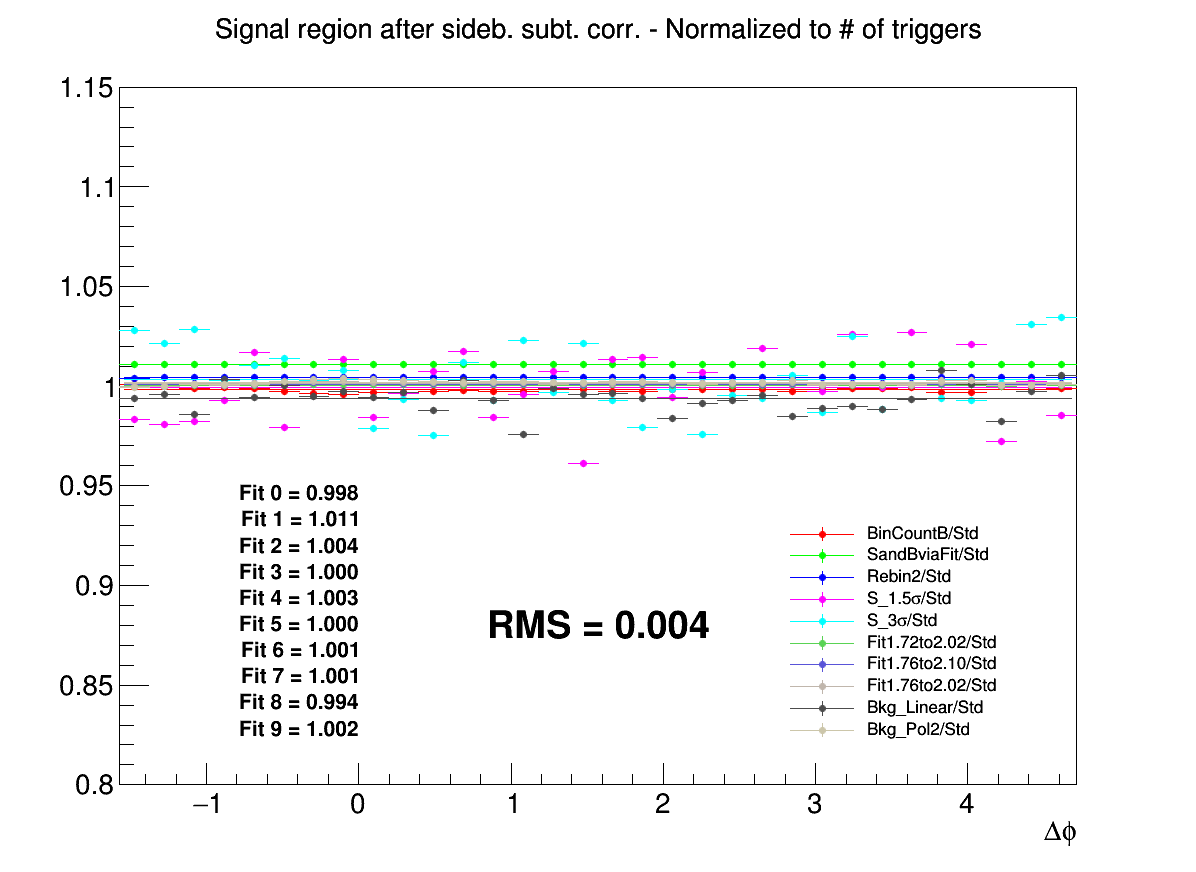
\includegraphics[width=0.31\linewidth]{figures/Systematics/Dzero/Yield/Ratio_AzimCorrDistr_Dzero_Canvas_PtIntBins4to5_PoolInt_thr03to1.png}}
{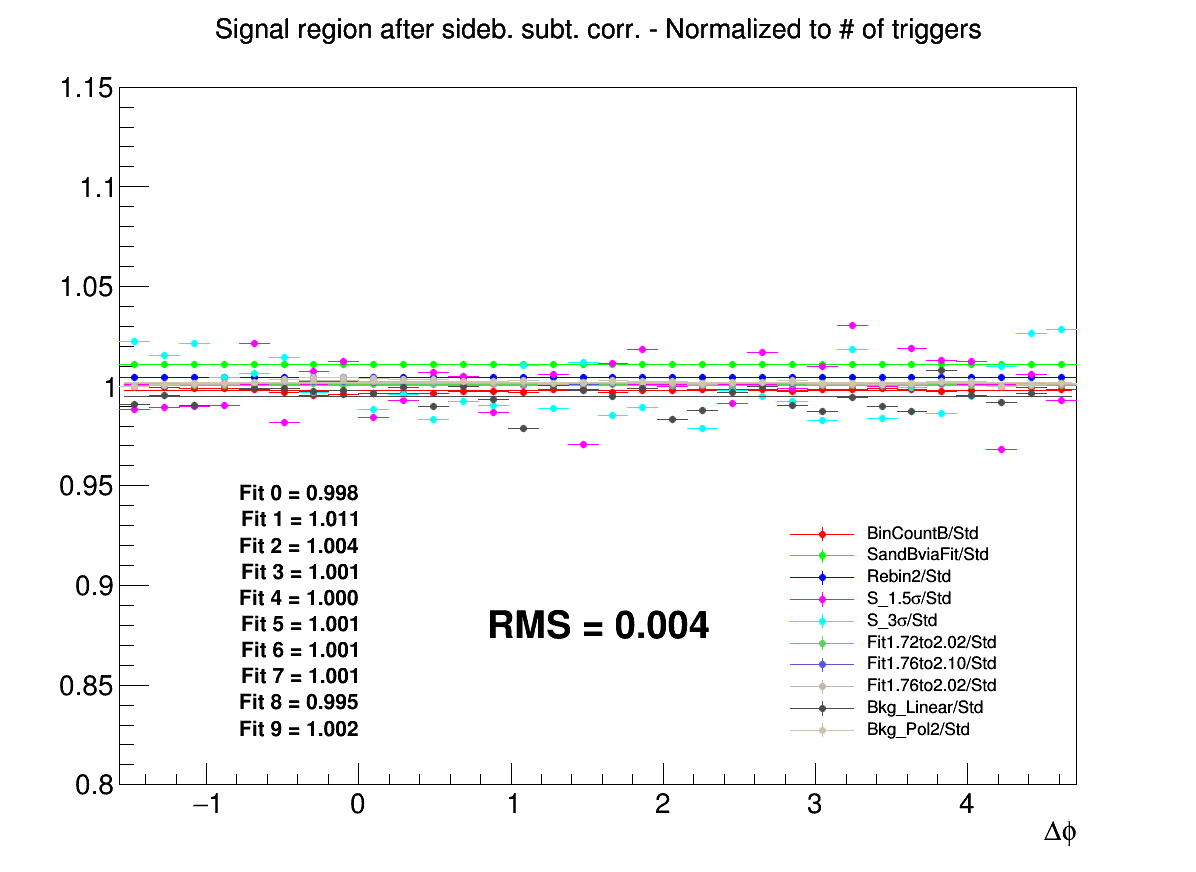
\includegraphics[width=0.31\linewidth]{figures/Systematics/Dzero/Yield/Ratio_AzimCorrDistr_Dzero_Canvas_PtIntBins4to5_PoolInt_thr03to99.png}}
{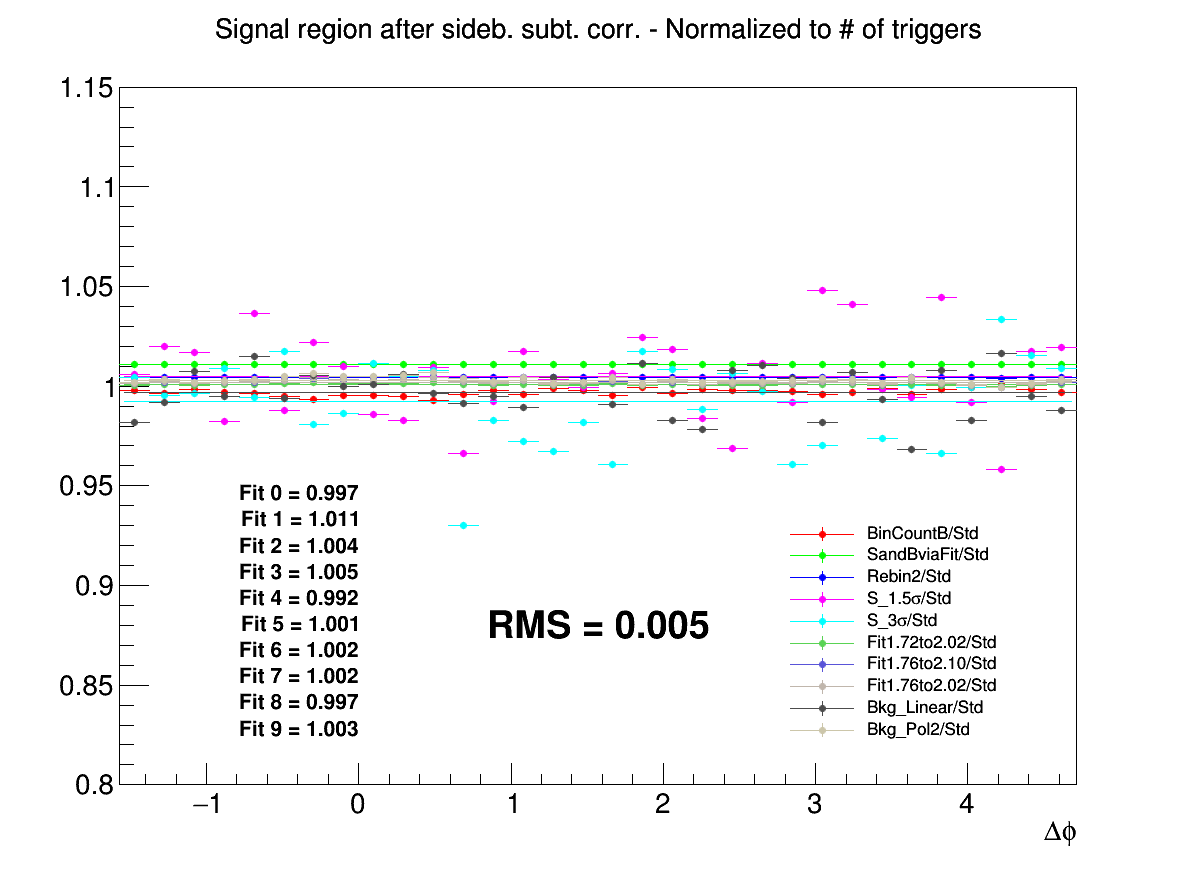
\includegraphics[width=0.31\linewidth]{figures/Systematics/Dzero/Yield/Ratio_AzimCorrDistr_Dzero_Canvas_PtIntBins4to5_PoolInt_thr1to99.png}}
{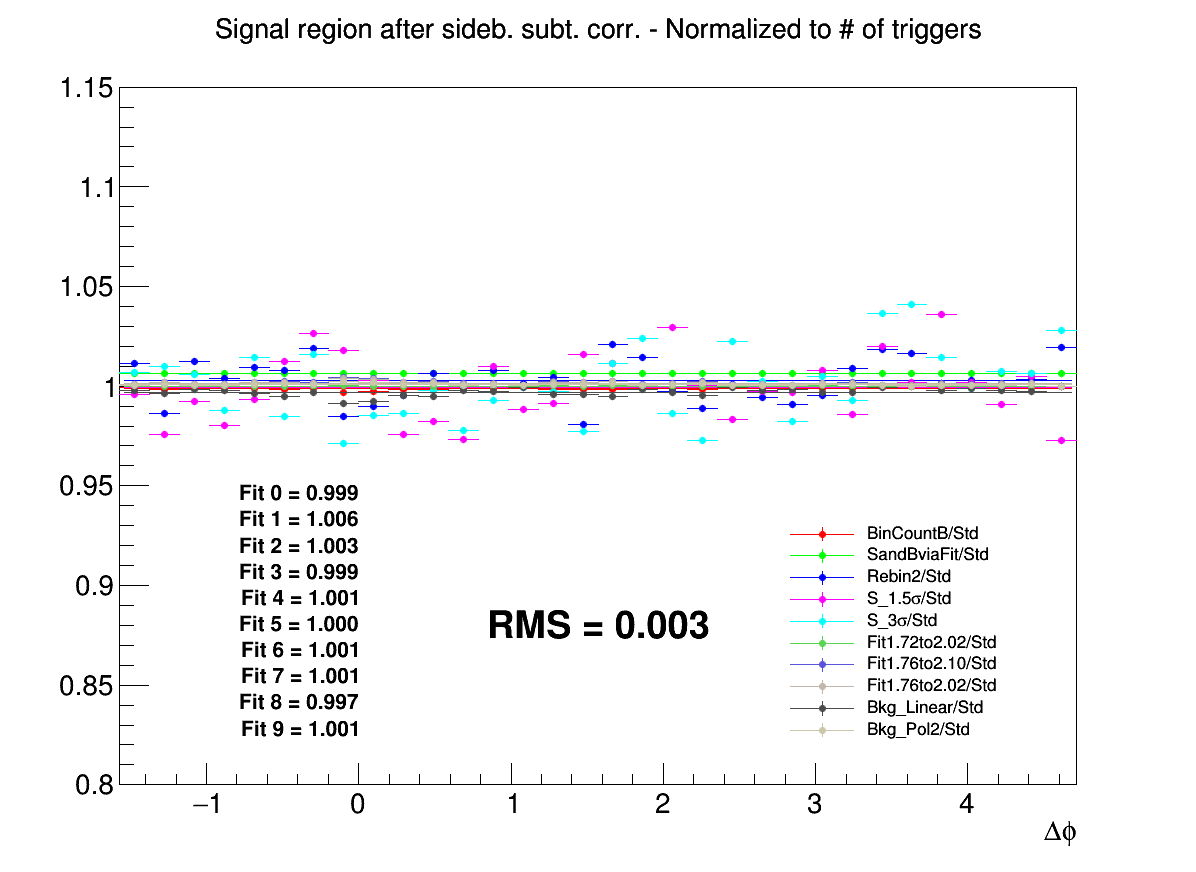
\includegraphics[width=0.31\linewidth]{figures/Systematics/Dzero/Yield/Ratio_AzimCorrDistr_Dzero_Canvas_PtIntBins6to8_PoolInt_thr03to1.png}}
{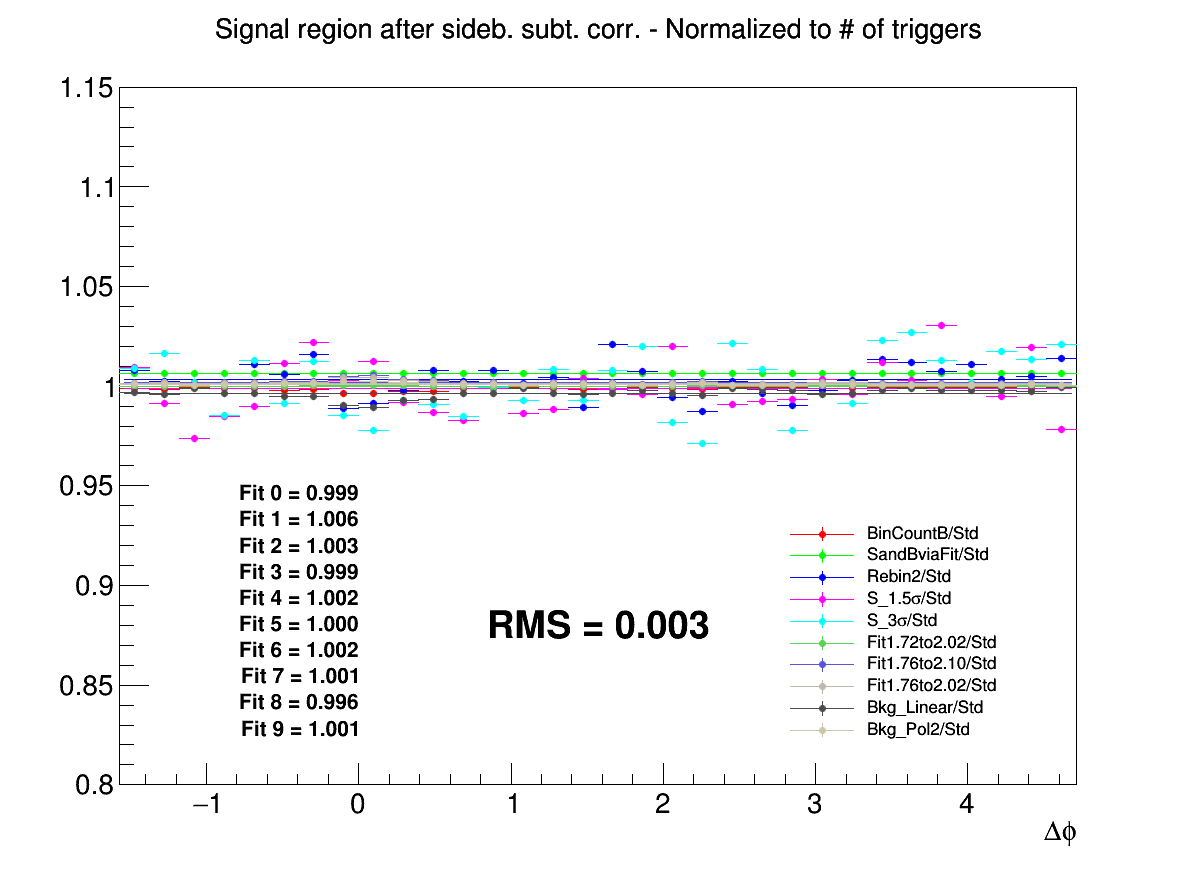
\includegraphics[width=0.31\linewidth]{figures/Systematics/Dzero/Yield/Ratio_AzimCorrDistr_Dzero_Canvas_PtIntBins6to8_PoolInt_thr03to99.png}}
{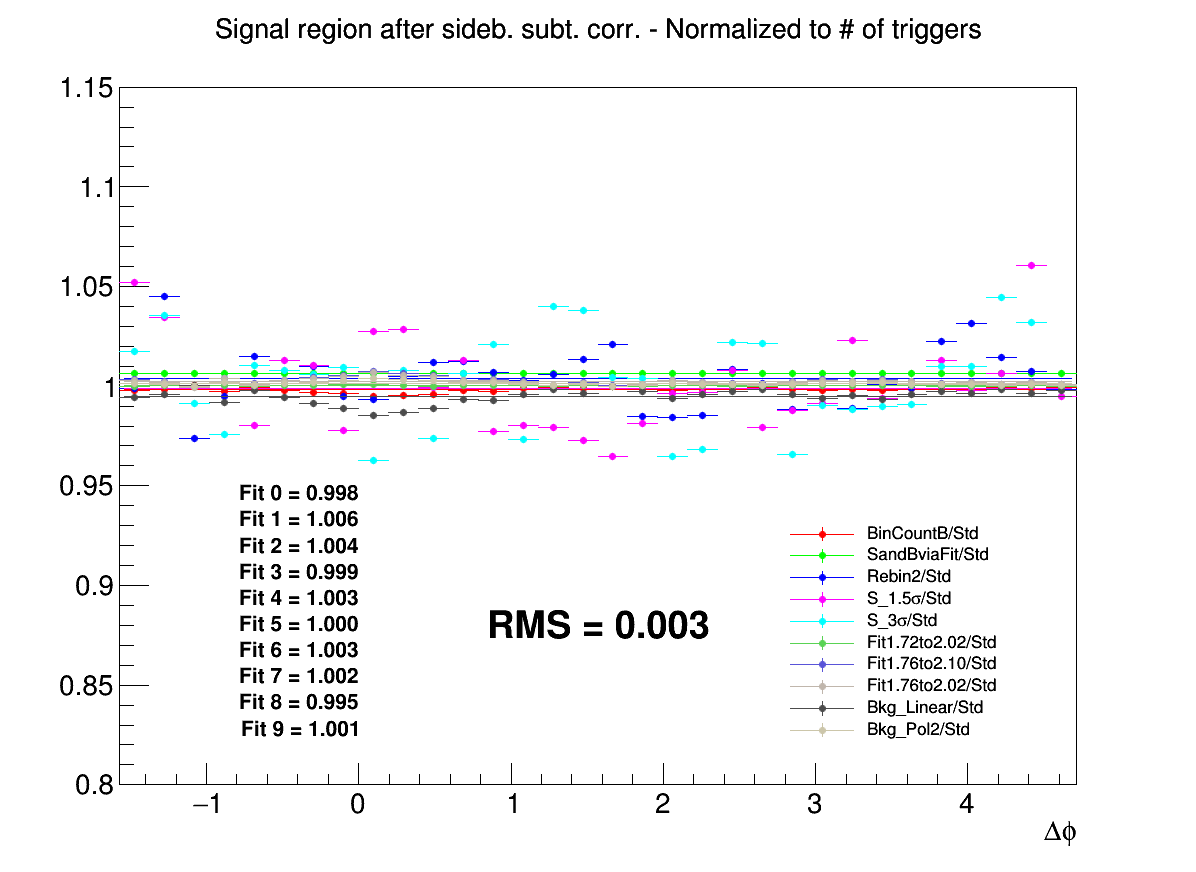
\includegraphics[width=0.31\linewidth]{figures/Systematics/Dzero/Yield/Ratio_AzimCorrDistr_Dzero_Canvas_PtIntBins6to8_PoolInt_thr1to99.png}}
{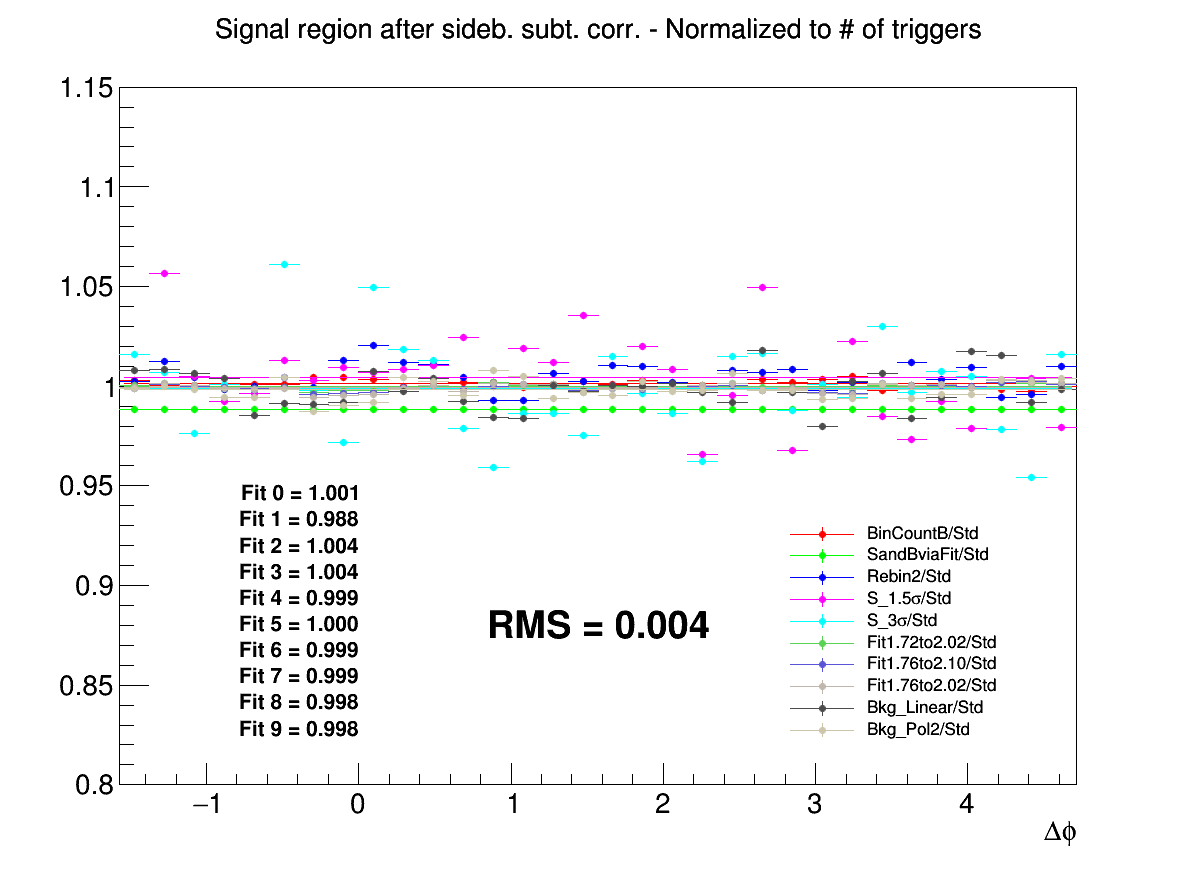
\includegraphics[width=0.31\linewidth]{figures/Systematics/Dzero/Yield/Ratio_AzimCorrDistr_Dzero_Canvas_PtIntBins9to11_PoolInt_thr03to1.png}}
{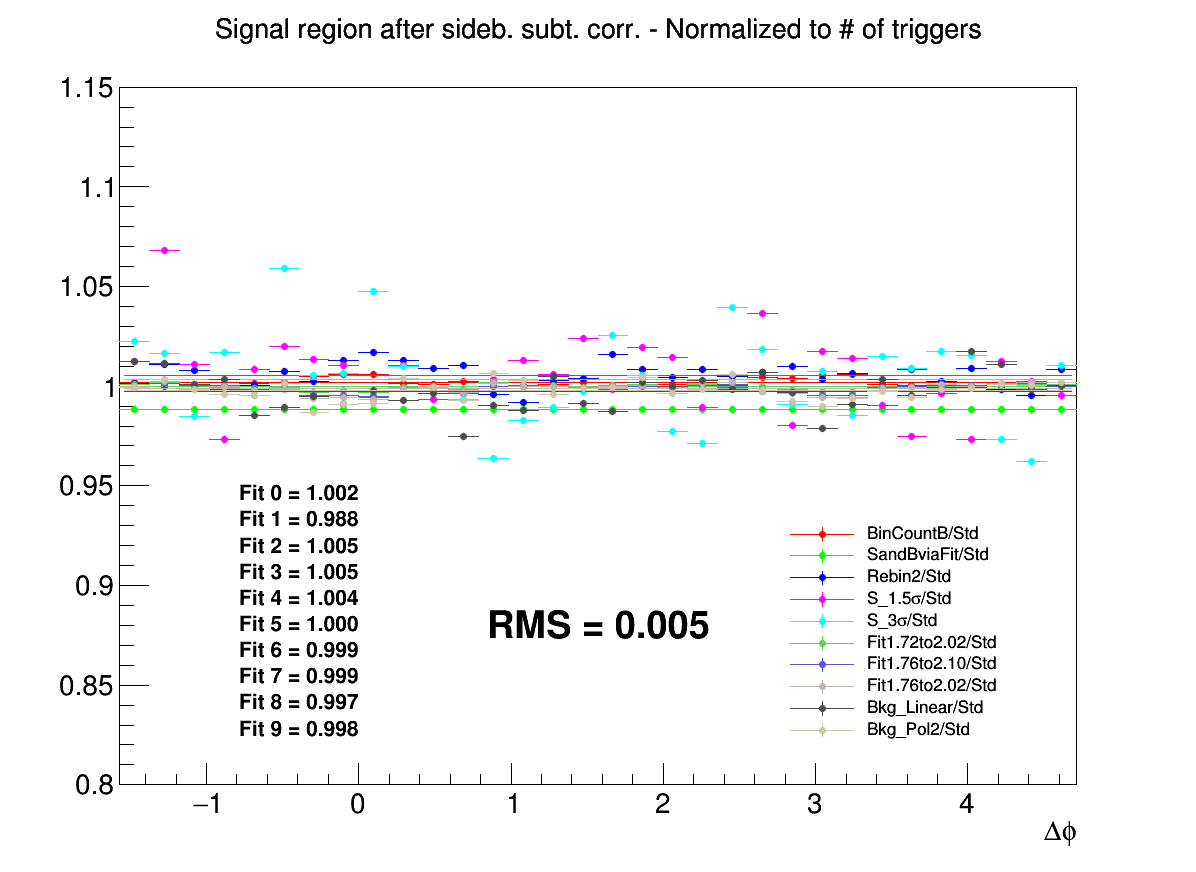
\includegraphics[width=0.31\linewidth]{figures/Systematics/Dzero/Yield/Ratio_AzimCorrDistr_Dzero_Canvas_PtIntBins9to11_PoolInt_thr03to99.png}}
{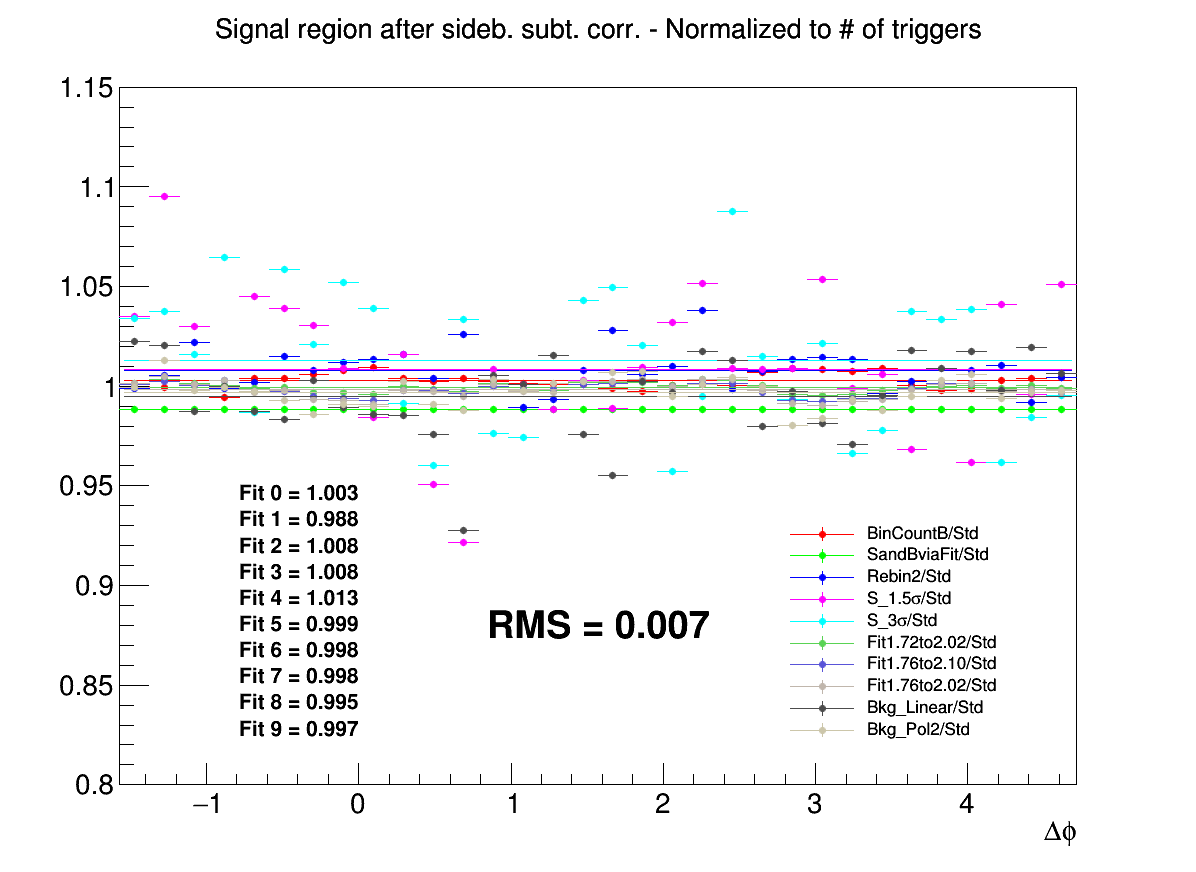
\includegraphics[width=0.31\linewidth]{figures/Systematics/Dzero/Yield/Ratio_AzimCorrDistr_Dzero_Canvas_PtIntBins9to11_PoolInt_thr1to99.png}}
{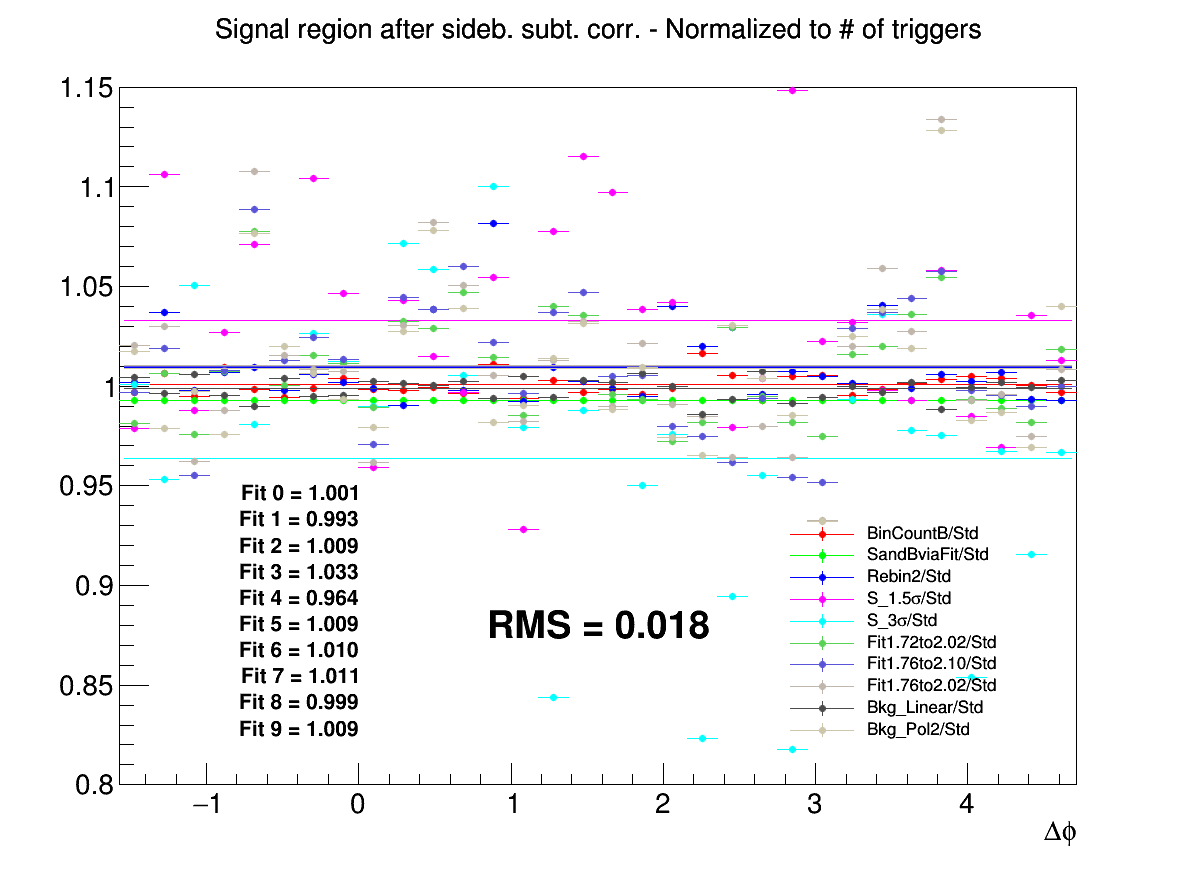
\includegraphics[width=0.31\linewidth]{figures/Systematics/Dzero/Yield/Ratio_AzimCorrDistr_Dzero_Canvas_PtIntBins12to13_PoolInt_thr03to1.png}}
{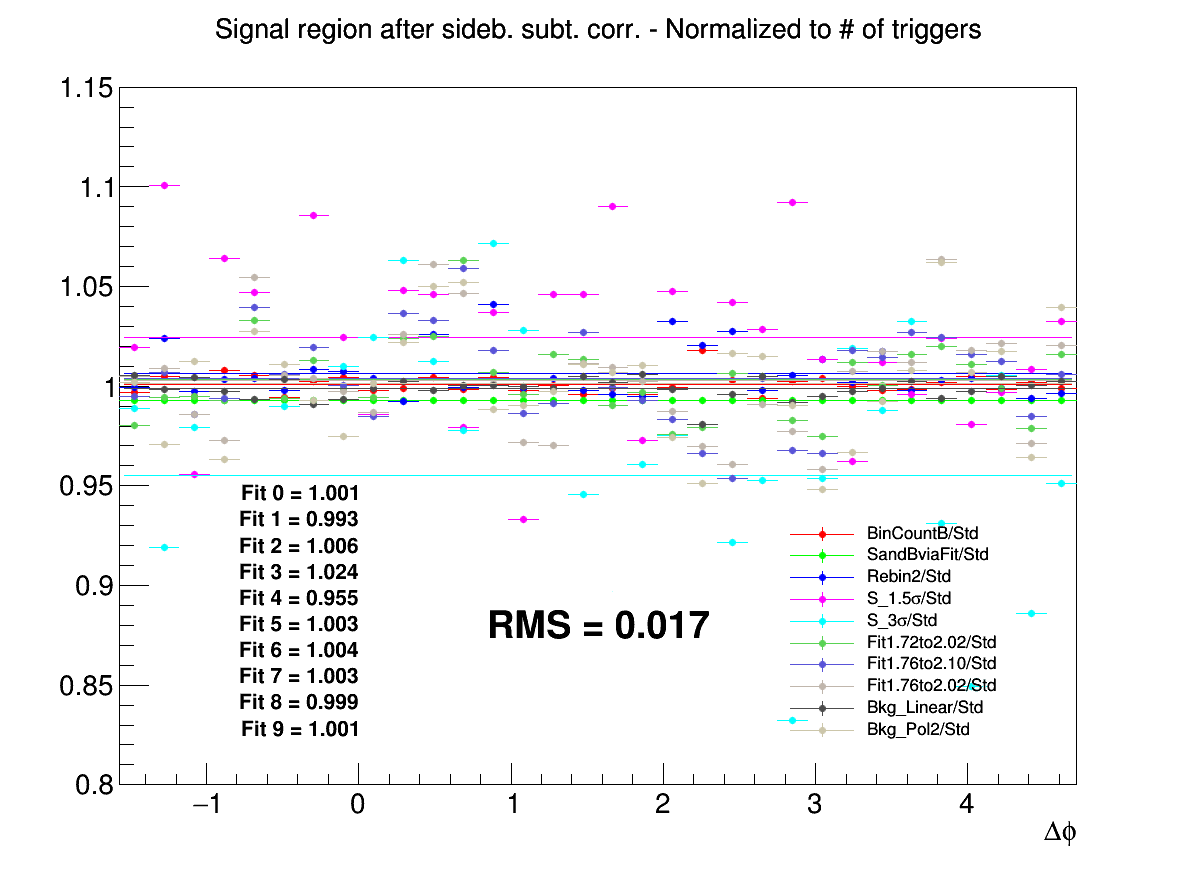
\includegraphics[width=0.31\linewidth]{figures/Systematics/Dzero/Yield/Ratio_AzimCorrDistr_Dzero_Canvas_PtIntBins12to13_PoolInt_thr03to99.png}}
{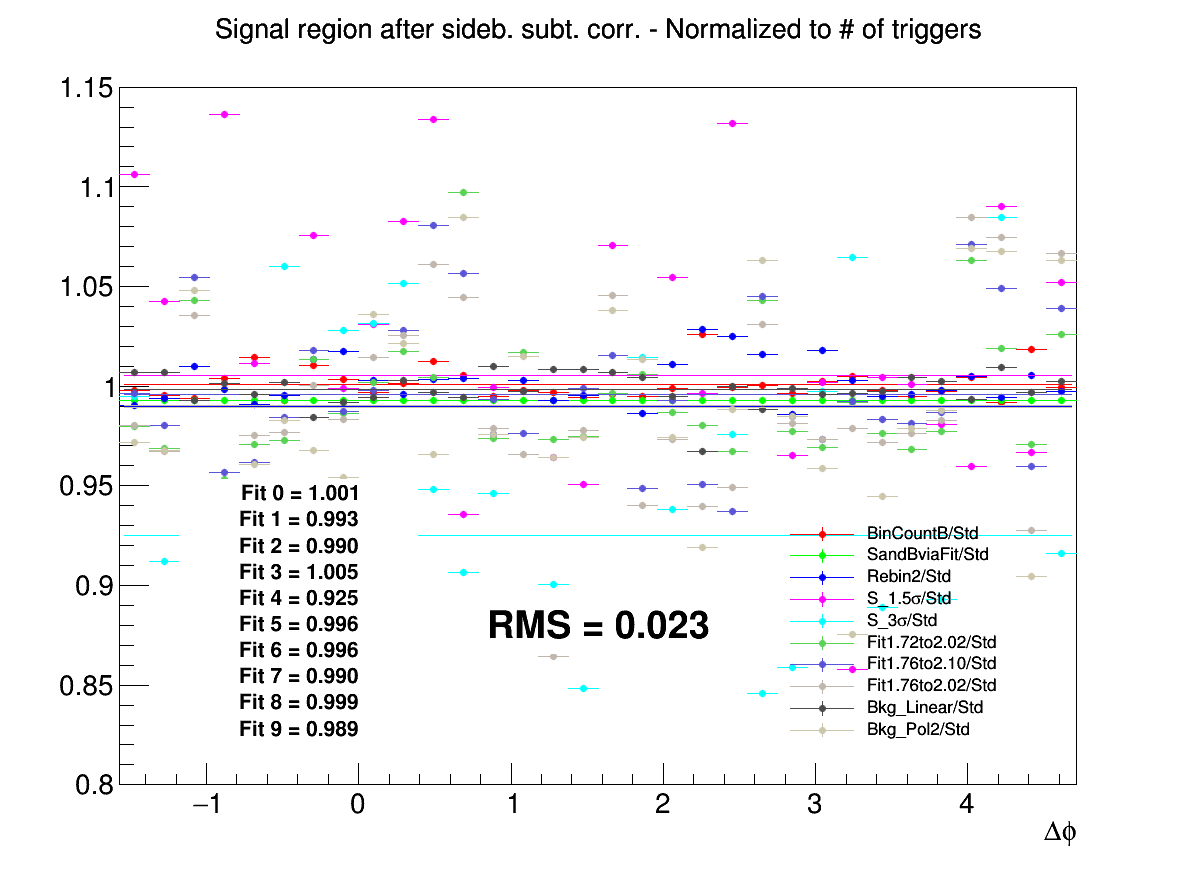
\includegraphics[width=0.31\linewidth]{figures/Systematics/Dzero/Yield/Ratio_AzimCorrDistr_Dzero_Canvas_PtIntBins12to13_PoolInt_thr1to99.png}}
 \caption{Ratios of $\Dzero$-h correlation plots obtained changing S and B extraction procedure over those obtained with standard yield extraction procedure. Rows: $\pt$($\Dzero$) 3-5, 5-8, 8-16, 16-24 $\gev/c$. In each row, the panels show the associated track $\pt$ ranges 0.3-1 $\gev/c$, $>$0.3 $\gev/c$, and $>$1 $\gev/c$, respectively.}
\label{fig:Syst_D0Yield}
\end{figure}

\begin{figure}
\centering
{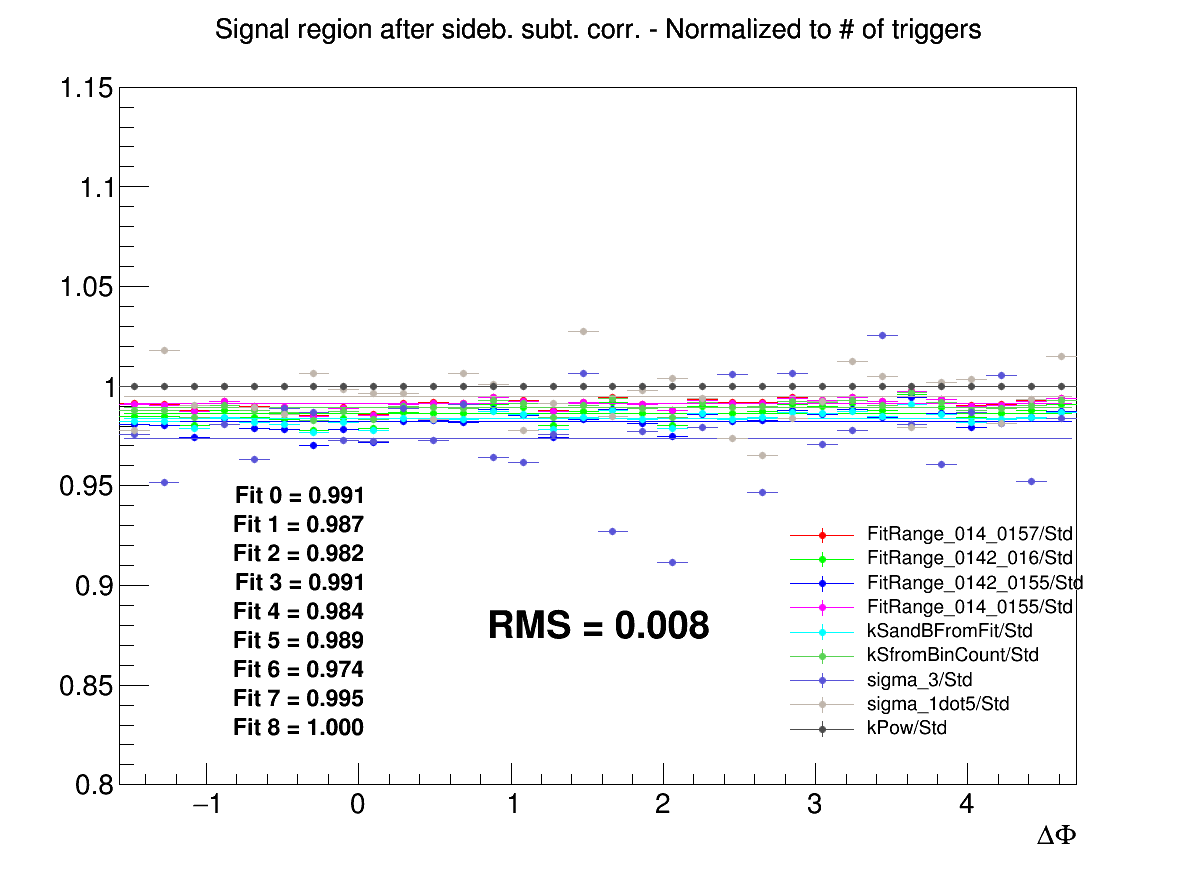
\includegraphics[width=0.31\linewidth]{figures/Systematics/Dstar/Yield/Ratio_AzimCorrDistr_Dstar_Canvas_PtIntBins2to3_PoolInt_thrdot3to1dot_SandB.png}}
{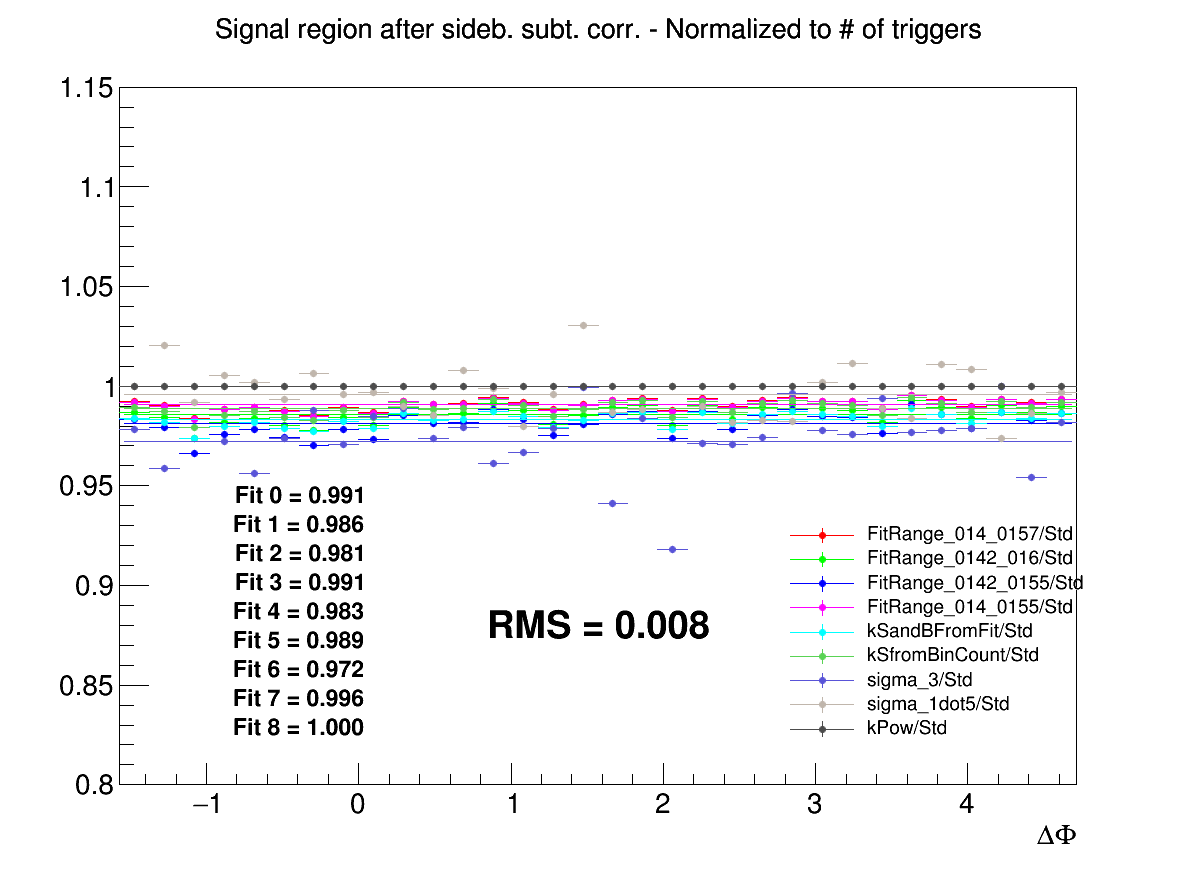
\includegraphics[width=0.31\linewidth]{figures/Systematics/Dstar/Yield/Ratio_AzimCorrDistr_Dstar_Canvas_PtIntBins2to3_PoolInt_thrdot3to99dot_SandB.png}}
{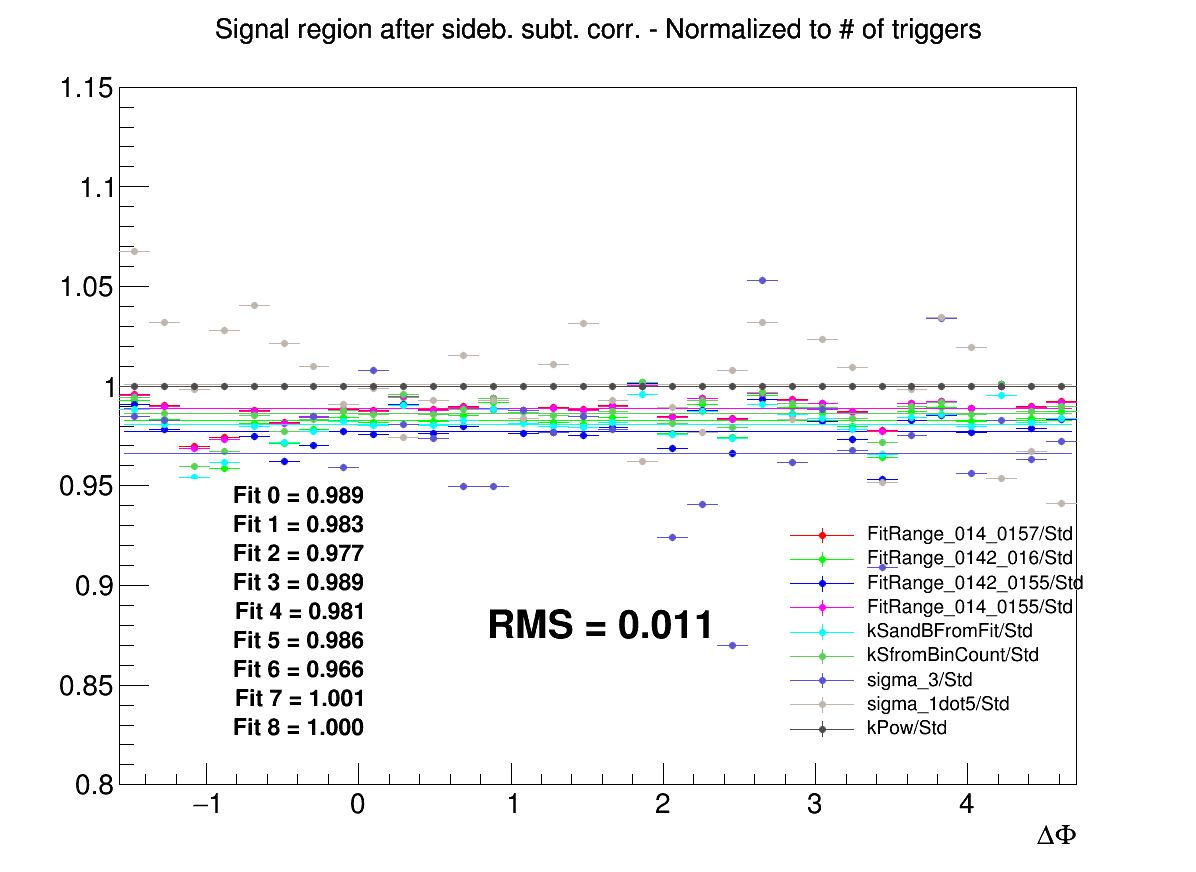
\includegraphics[width=0.31\linewidth]{figures/Systematics/Dstar/Yield/Ratio_AzimCorrDistr_Dstar_Canvas_PtIntBins2to3_PoolInt_thr1dotto99dot_SandB.png}}
{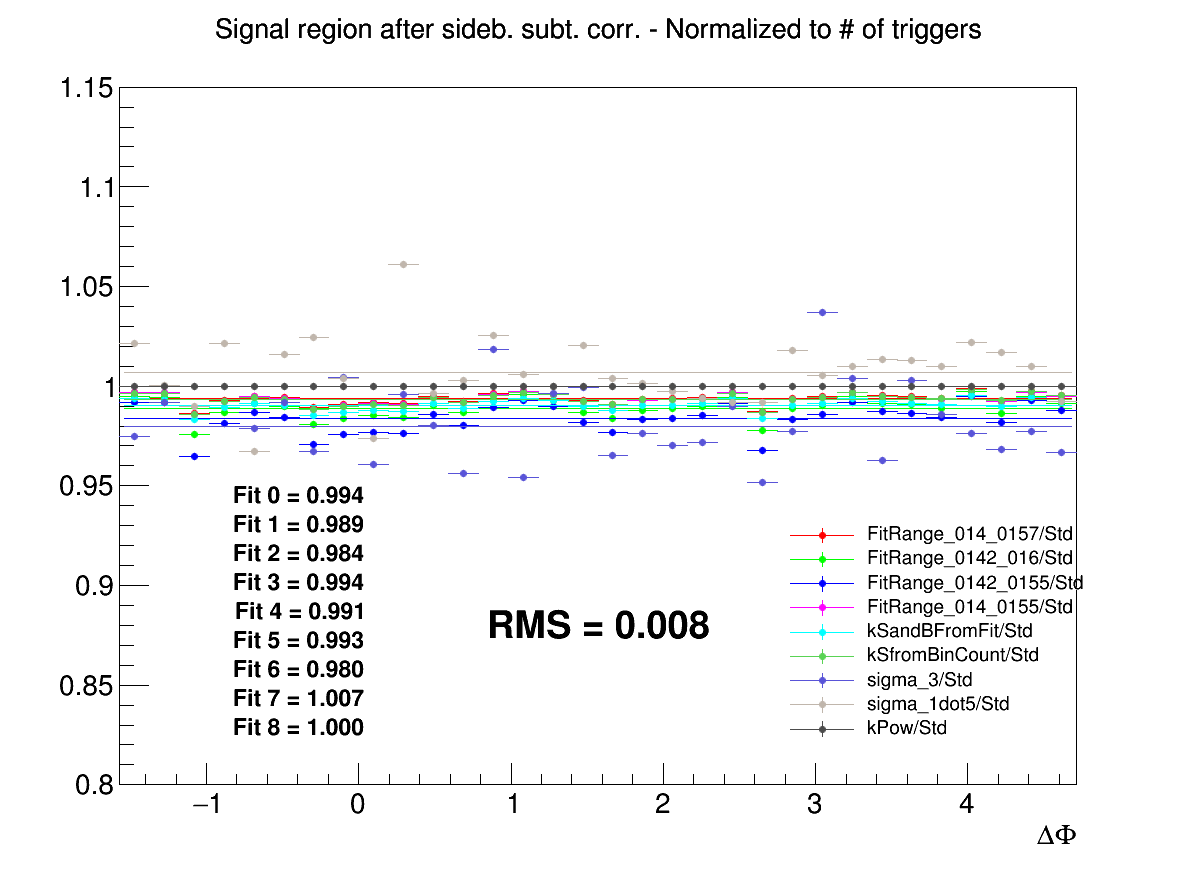
\includegraphics[width=0.31\linewidth]{figures/Systematics/Dstar/Yield/Ratio_AzimCorrDistr_Dstar_Canvas_PtIntBins4to6_PoolInt_thrdot3to1dot_SandB.png}}
{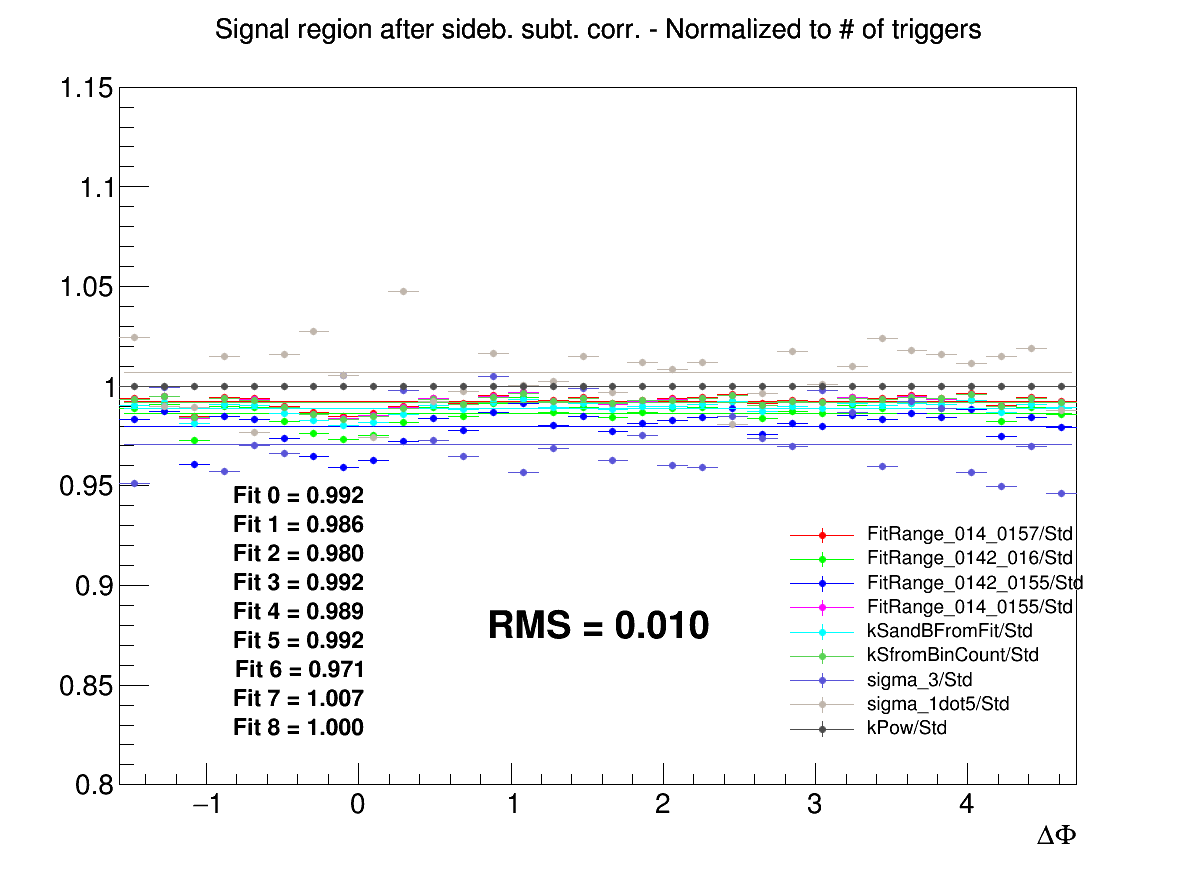
\includegraphics[width=0.31\linewidth]{figures/Systematics/Dstar/Yield/Ratio_AzimCorrDistr_Dstar_Canvas_PtIntBins4to6_PoolInt_thrdot3to99dot_SandB.png}}
{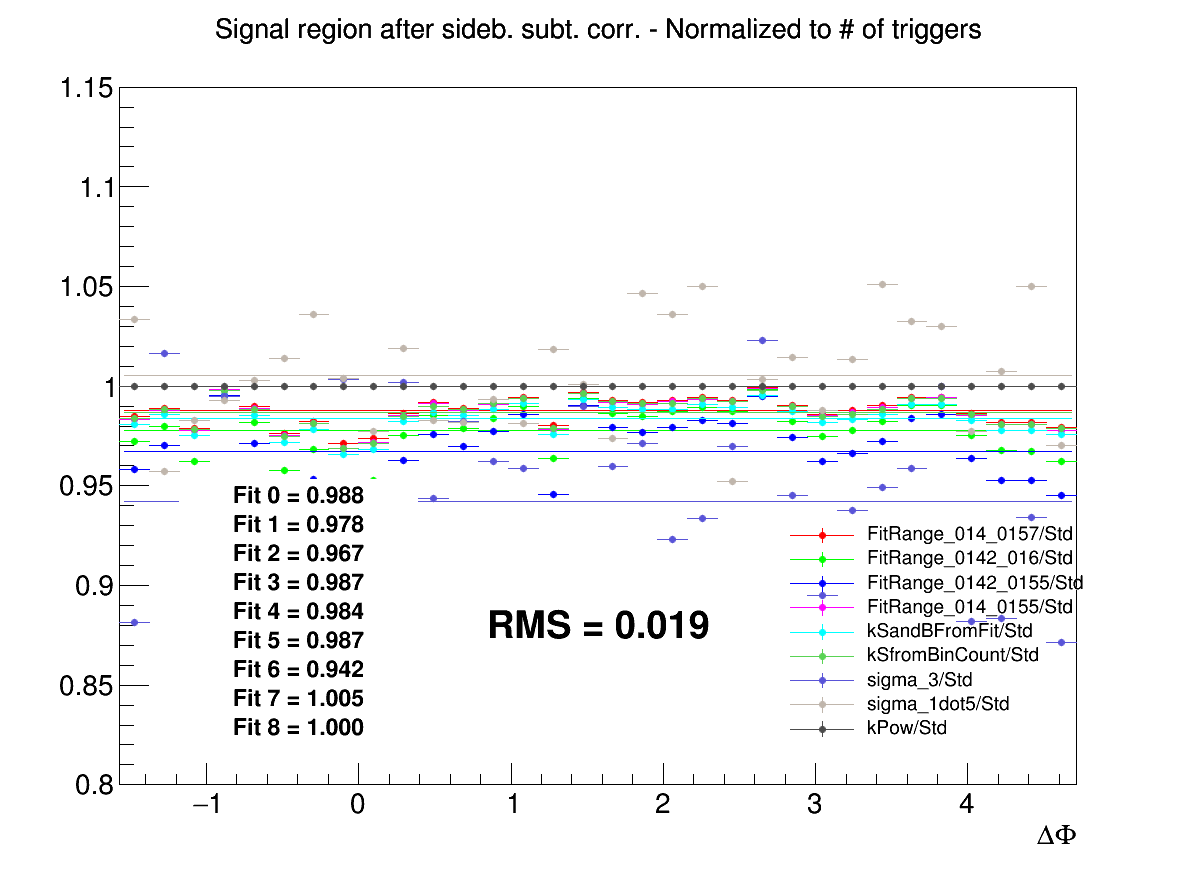
\includegraphics[width=0.31\linewidth]{figures/Systematics/Dstar/Yield/Ratio_AzimCorrDistr_Dstar_Canvas_PtIntBins4to6_PoolInt_thr1dotto99dot_SandB.png}}
{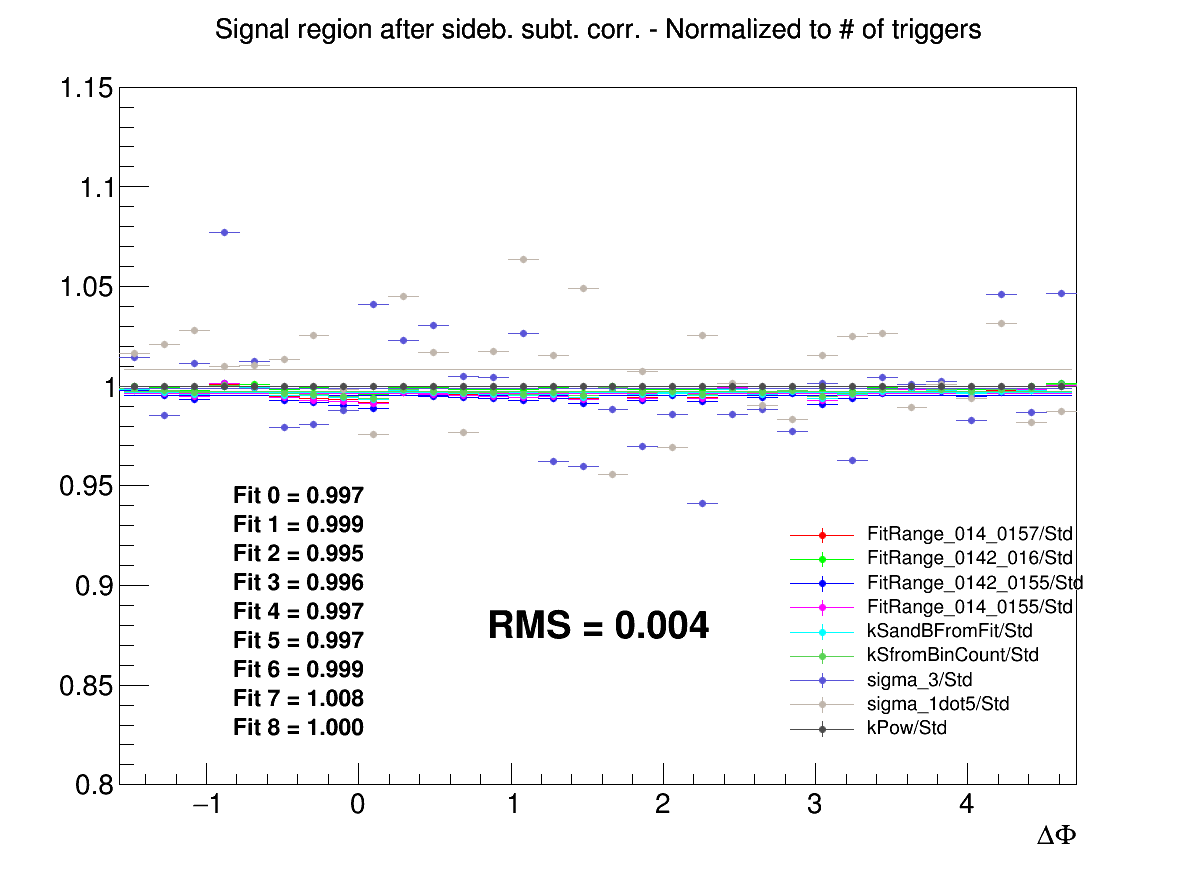
\includegraphics[width=0.31\linewidth]{figures/Systematics/Dstar/Yield/Ratio_AzimCorrDistr_Dstar_Canvas_PtIntBins7to9_PoolInt_thrdot3to1dot_SandB.png}}
{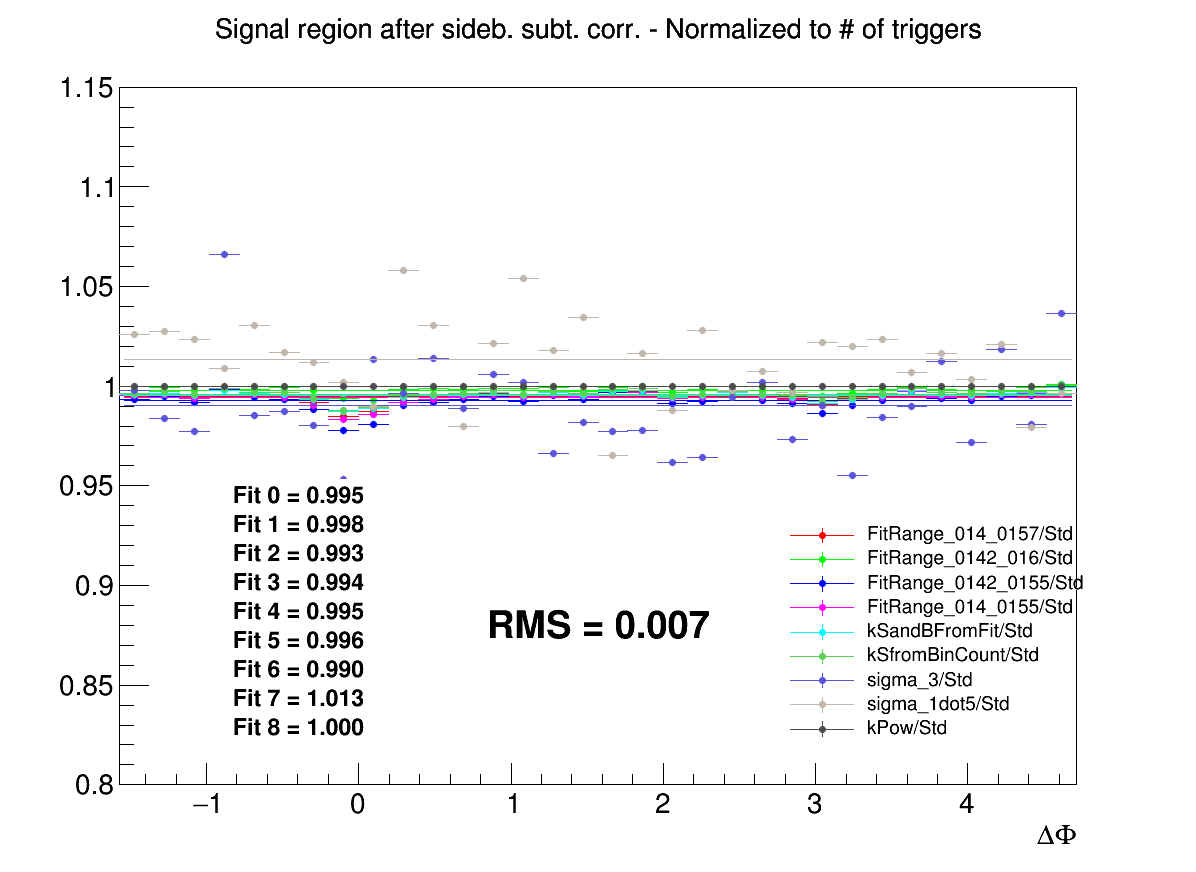
\includegraphics[width=0.31\linewidth]{figures/Systematics/Dstar/Yield/Ratio_AzimCorrDistr_Dstar_Canvas_PtIntBins7to9_PoolInt_thrdot3to99dot_SandB.png}}
{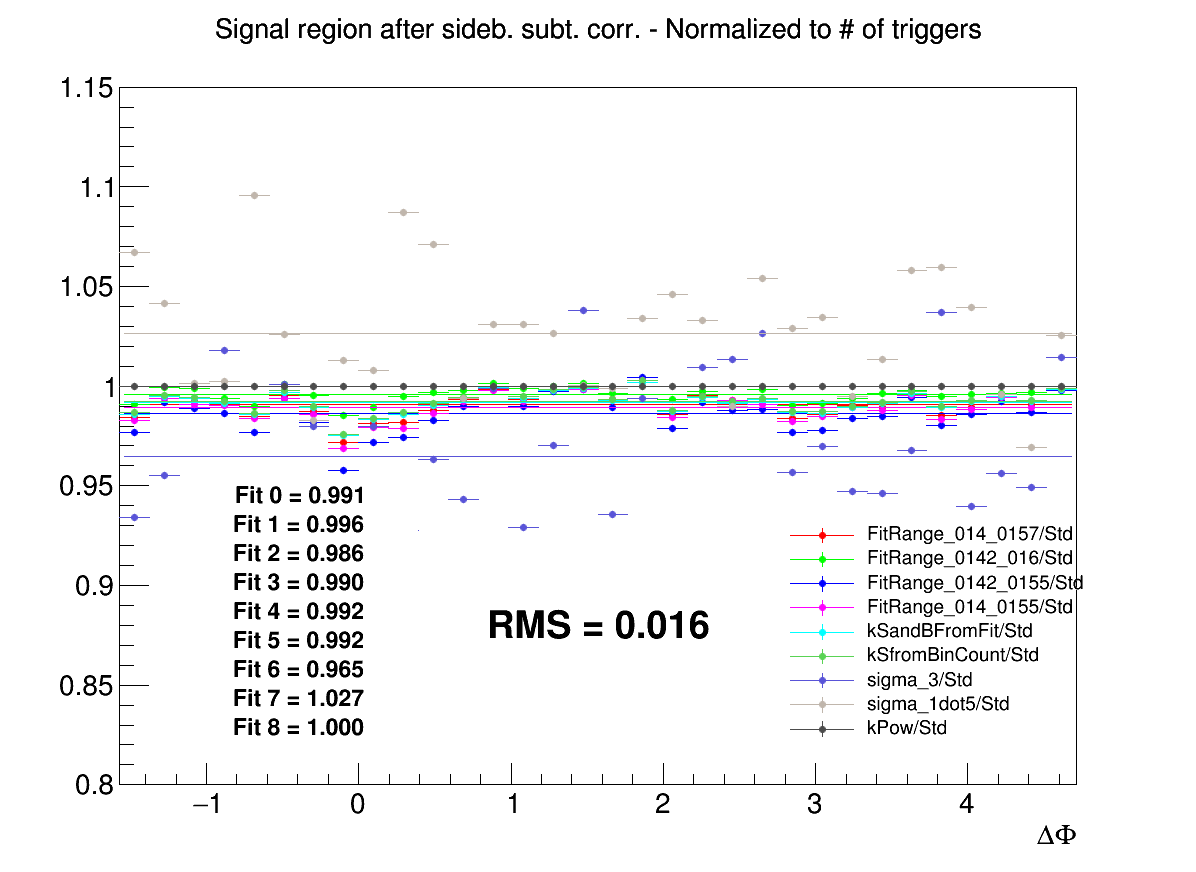
\includegraphics[width=0.31\linewidth]{figures/Systematics/Dstar/Yield/Ratio_AzimCorrDistr_Dstar_Canvas_PtIntBins7to9_PoolInt_thr1dotto99dot_SandB.png}}
{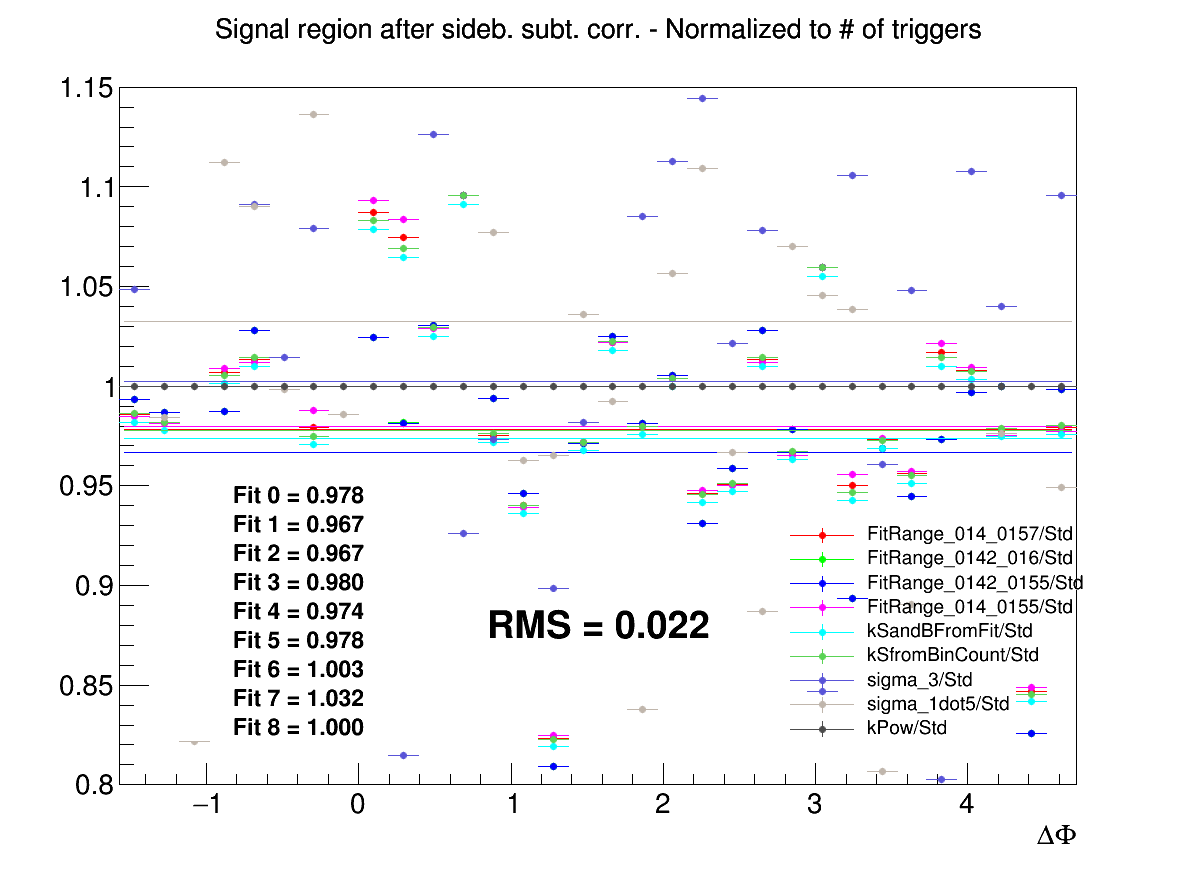
\includegraphics[width=0.31\linewidth]{figures/Systematics/Dstar/Yield/Ratio_AzimCorrDistr_Dstar_Canvas_PtIntBins10to10_PoolInt_thrdot3to1dot_SandB.png}}
{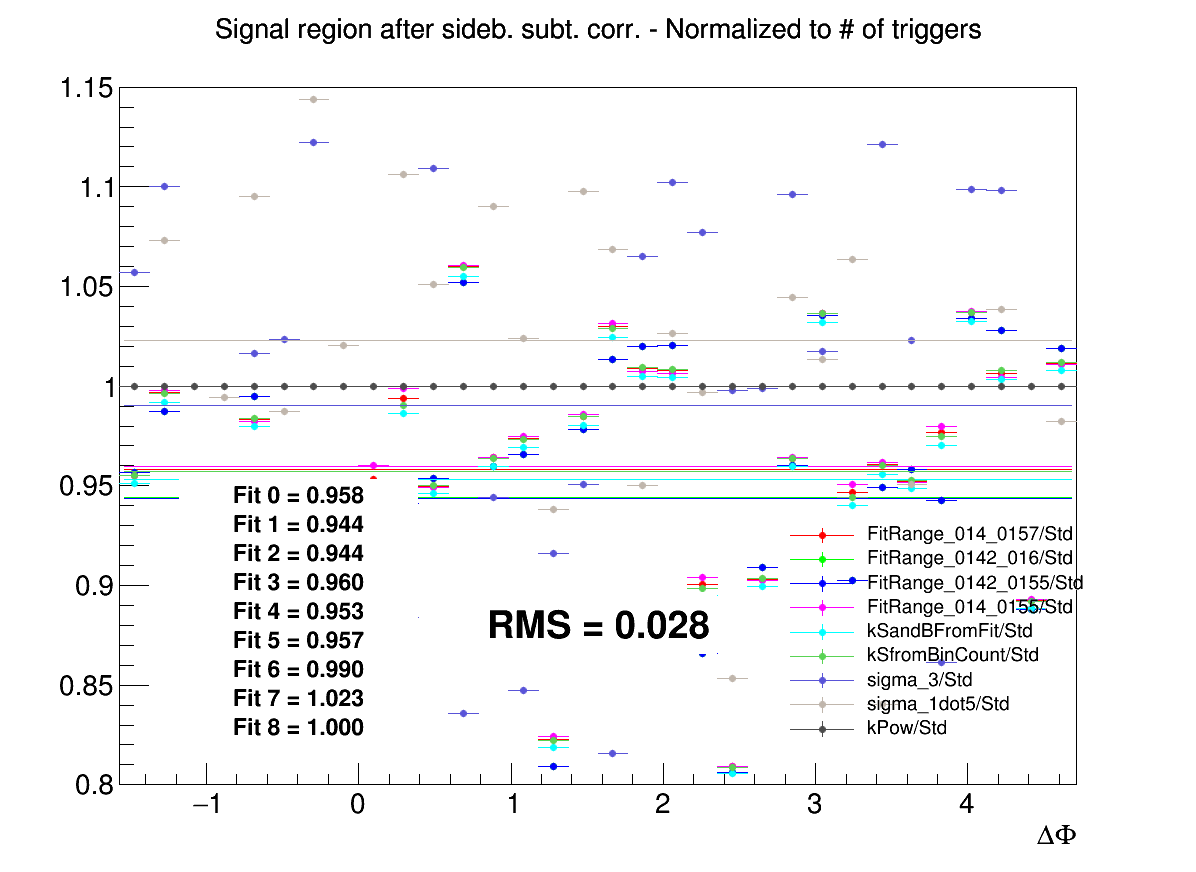
\includegraphics[width=0.31\linewidth]{figures/Systematics/Dstar/Yield/Ratio_AzimCorrDistr_Dstar_Canvas_PtIntBins10to10_PoolInt_thrdot3to99dot_SandB.png}}
{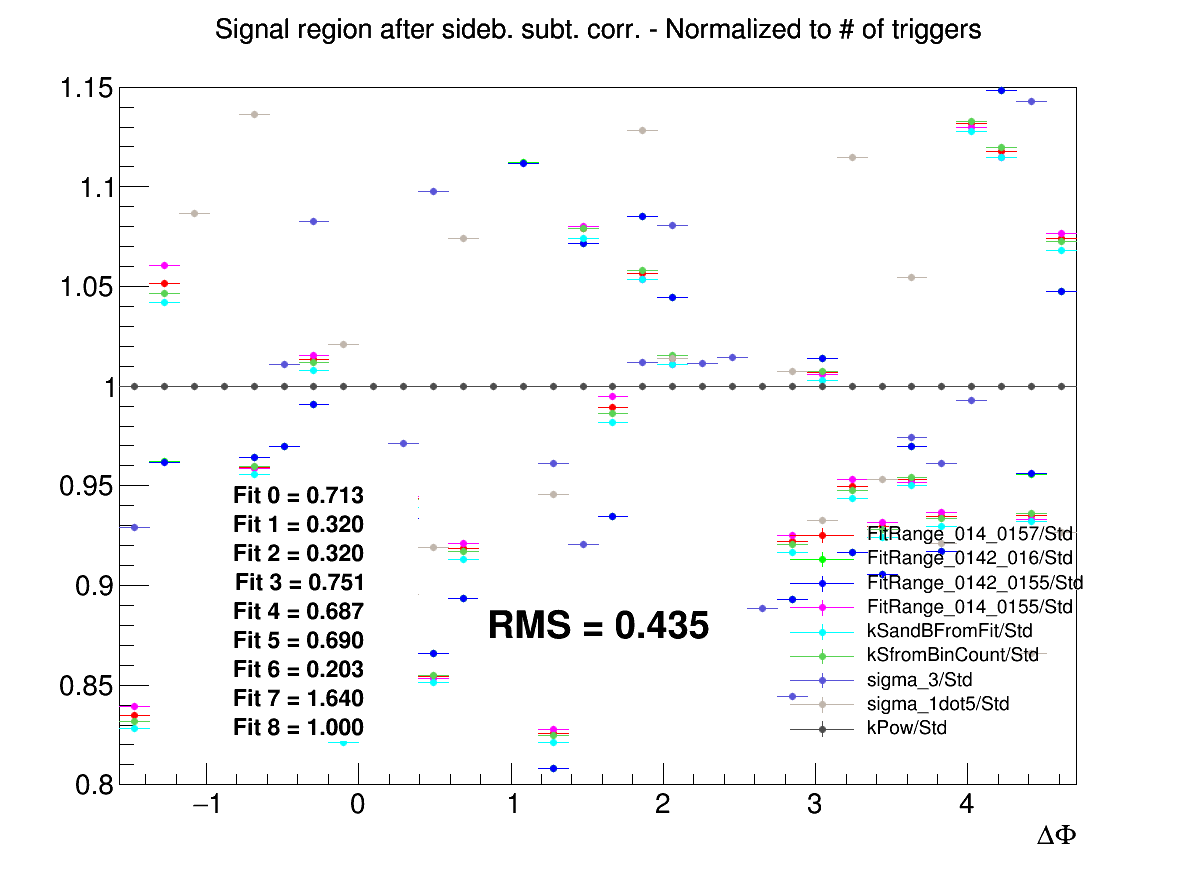
\includegraphics[width=0.31\linewidth]{figures/Systematics/Dstar/Yield/Ratio_AzimCorrDistr_Dstar_Canvas_PtIntBins10to10_PoolInt_thr1dotto99dot_SandB.png}}
\caption{Ratios of $\Dstar$-h correlation plots obtained changing S and B extraction procedure over those obtained with standard yield extraction procedure. Rows: $\pt$($\Dstar$) 3-5, 5-8, 8-16, 16-24 $\gev/c$. In each row, the panels show the associated track $\pt$ ranges $>$0.3 $\gev/c$, 0.3-1 $\gev/c$ and $>$1 $\gev/c$, respectively.}
\label{fig:Syst_DstarYield}
\end{figure}


\begin{figure}
\centering
{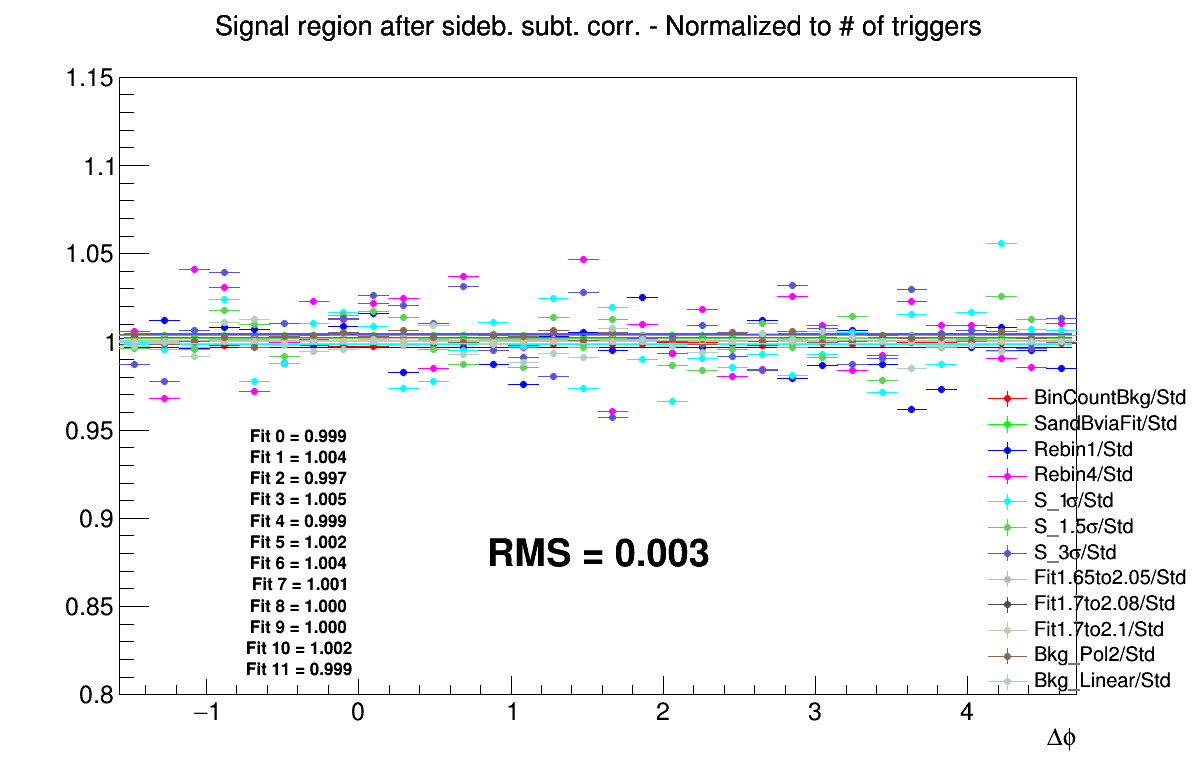
\includegraphics[width=0.31\linewidth]{figures/Systematics/Dplus/Yield/Ratio_AzimCorrDistr_Dplus_Canvas_PtIntBins3to4_PoolInt_thrdot3to1dot.png}}
{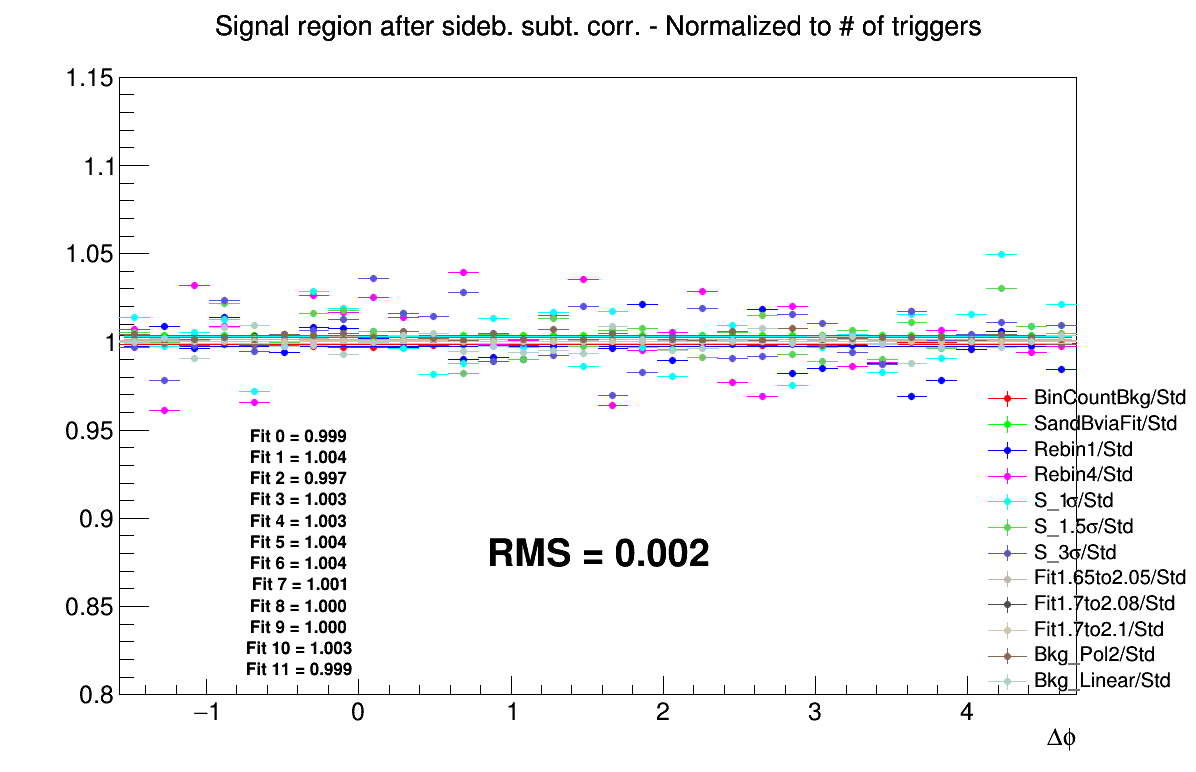
\includegraphics[width=0.31\linewidth]{figures/Systematics/Dplus/Yield/Ratio_AzimCorrDistr_Dplus_Canvas_PtIntBins3to4_PoolInt_thrdot3to99dot.png}}
{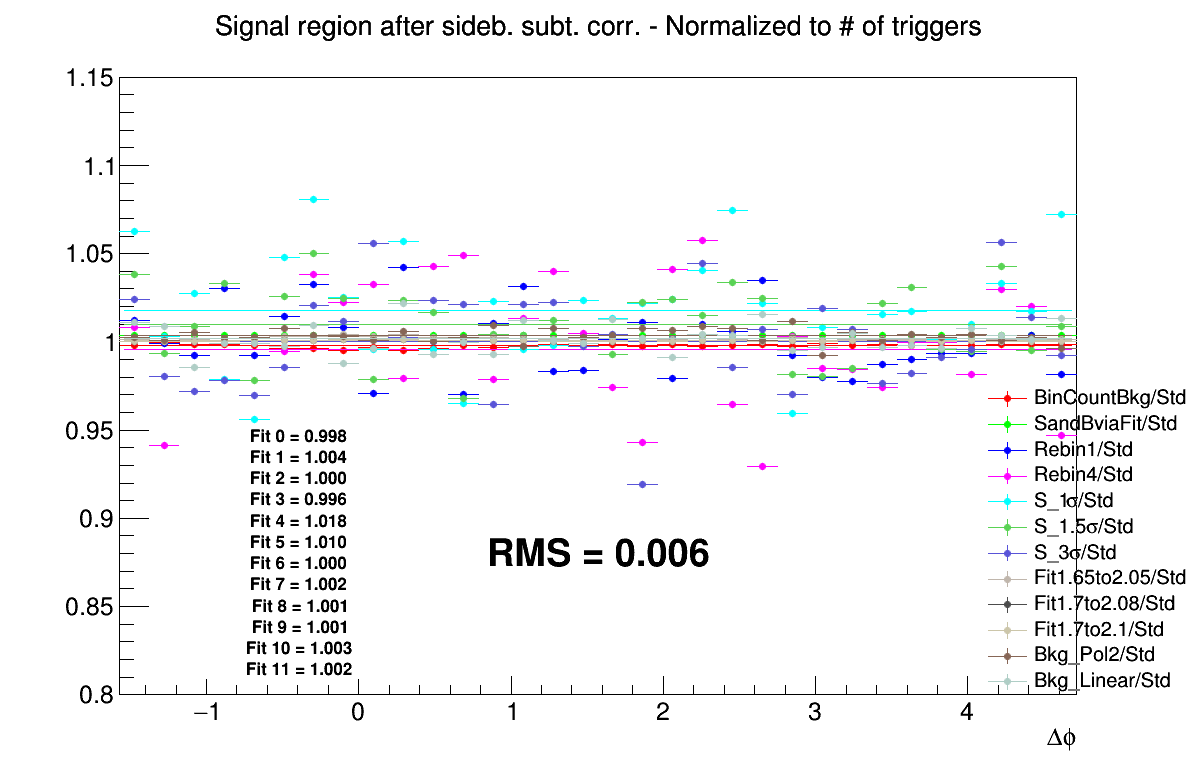
\includegraphics[width=0.31\linewidth]{figures/Systematics/Dplus/Yield/Ratio_AzimCorrDistr_Dplus_Canvas_PtIntBins3to4_PoolInt_thr1dotto99dot.png}}
{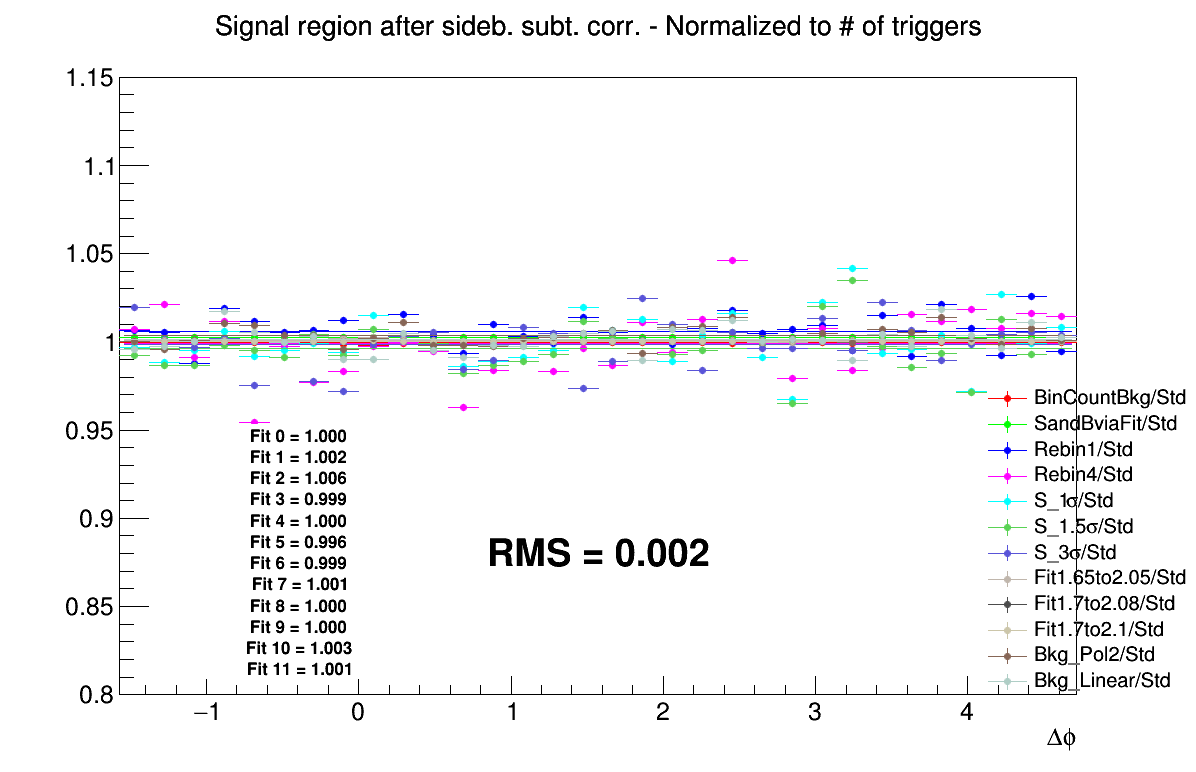
\includegraphics[width=0.31\linewidth]{figures/Systematics/Dplus/Yield/Ratio_AzimCorrDistr_Dplus_Canvas_PtIntBins5to7_PoolInt_thrdot3to1dot.png}}
{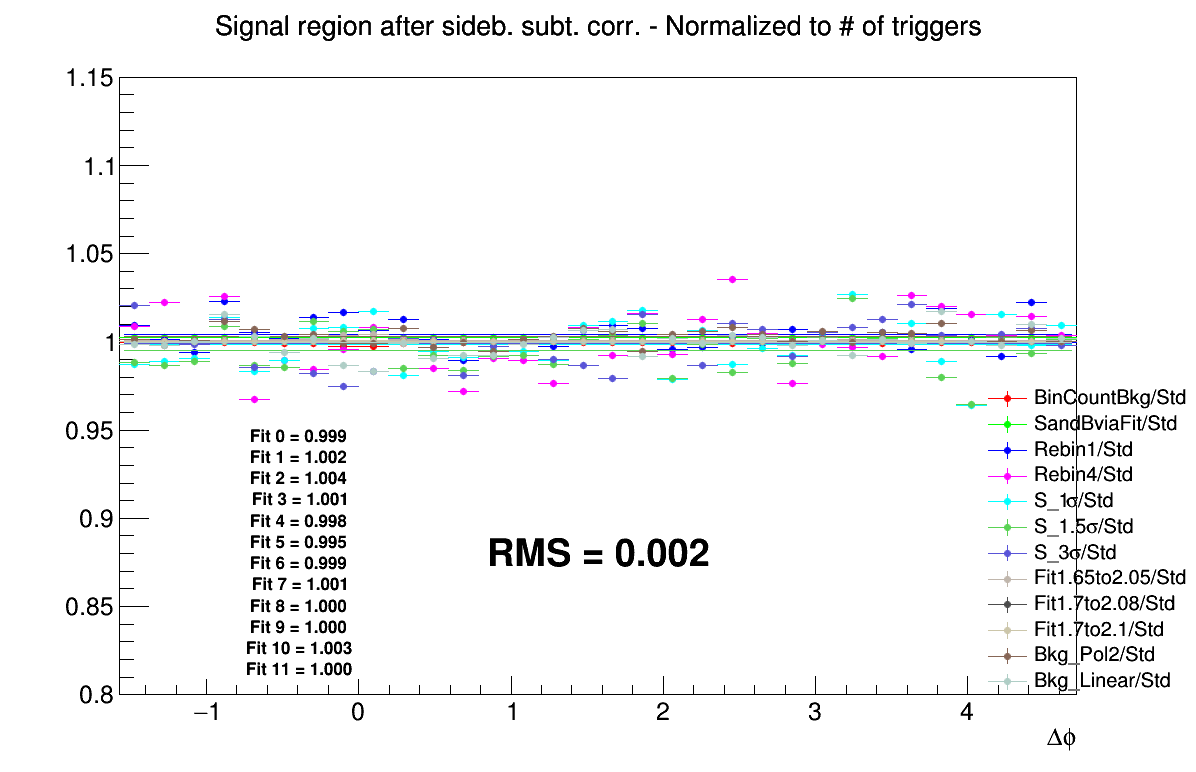
\includegraphics[width=0.31\linewidth]{figures/Systematics/Dplus/Yield/Ratio_AzimCorrDistr_Dplus_Canvas_PtIntBins5to7_PoolInt_thrdot3to99dot.png}}
{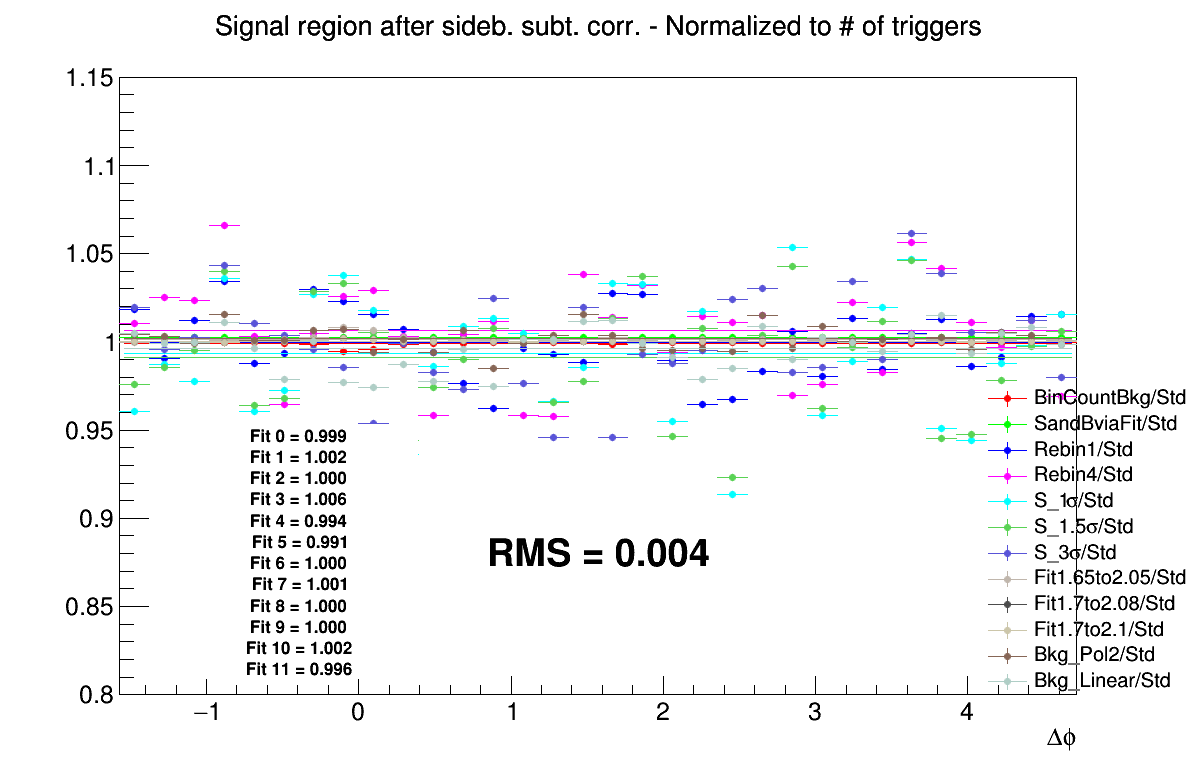
\includegraphics[width=0.31\linewidth]{figures/Systematics/Dplus/Yield/Ratio_AzimCorrDistr_Dplus_Canvas_PtIntBins5to7_PoolInt_thr1dotto99dot.png}}
{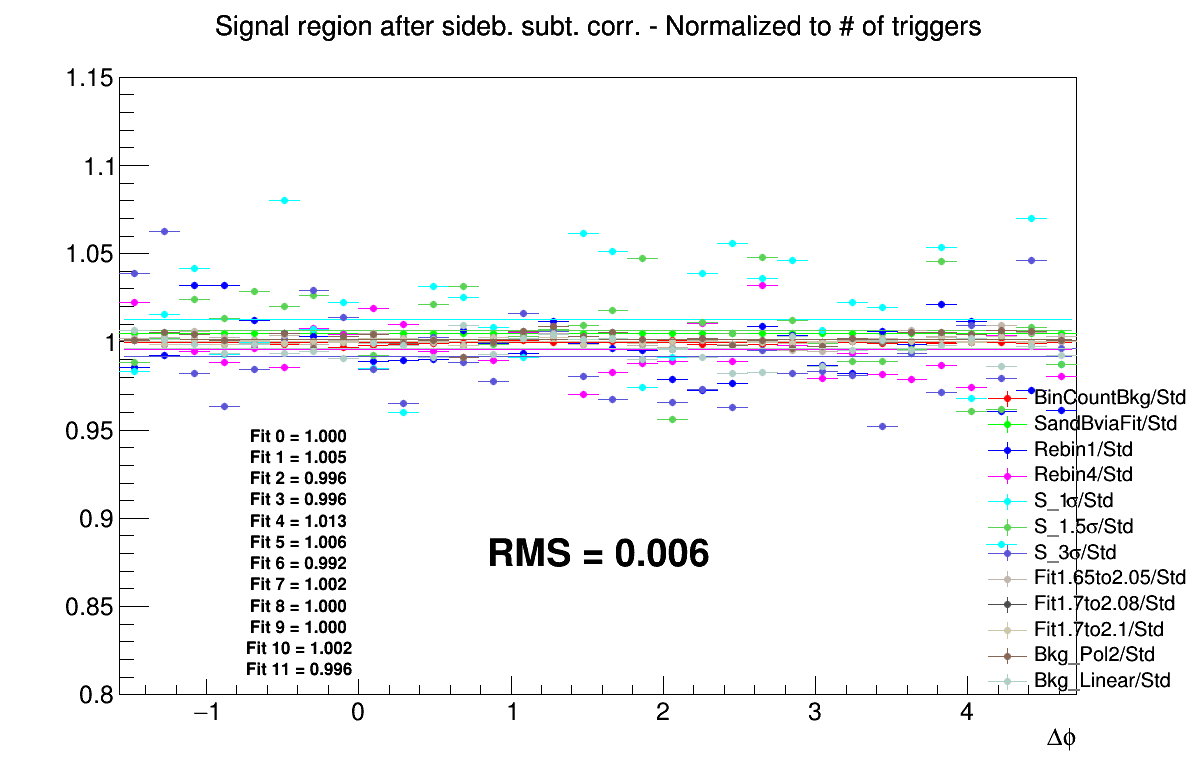
\includegraphics[width=0.31\linewidth]{figures/Systematics/Dplus/Yield/Ratio_AzimCorrDistr_Dplus_Canvas_PtIntBins8to12_PoolInt_thrdot3to1dot.png}}
{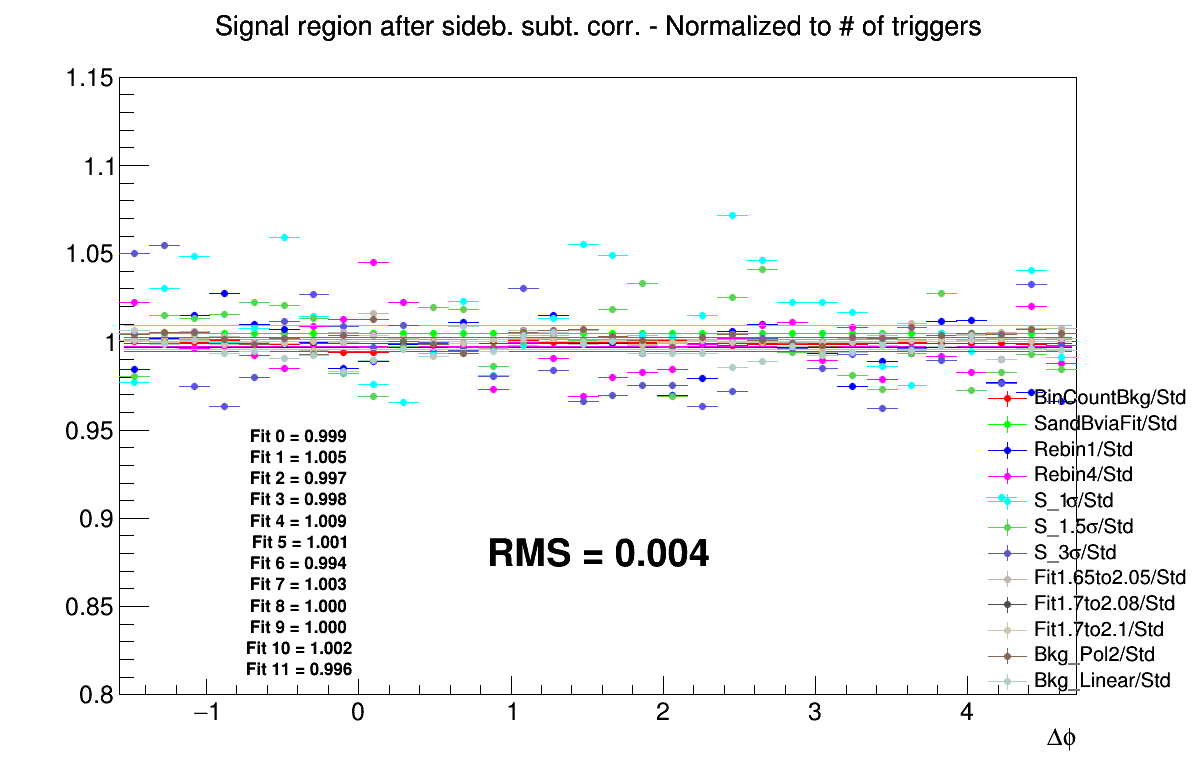
\includegraphics[width=0.31\linewidth]{figures/Systematics/Dplus/Yield/Ratio_AzimCorrDistr_Dplus_Canvas_PtIntBins8to12_PoolInt_thrdot3to99dot.png}}
{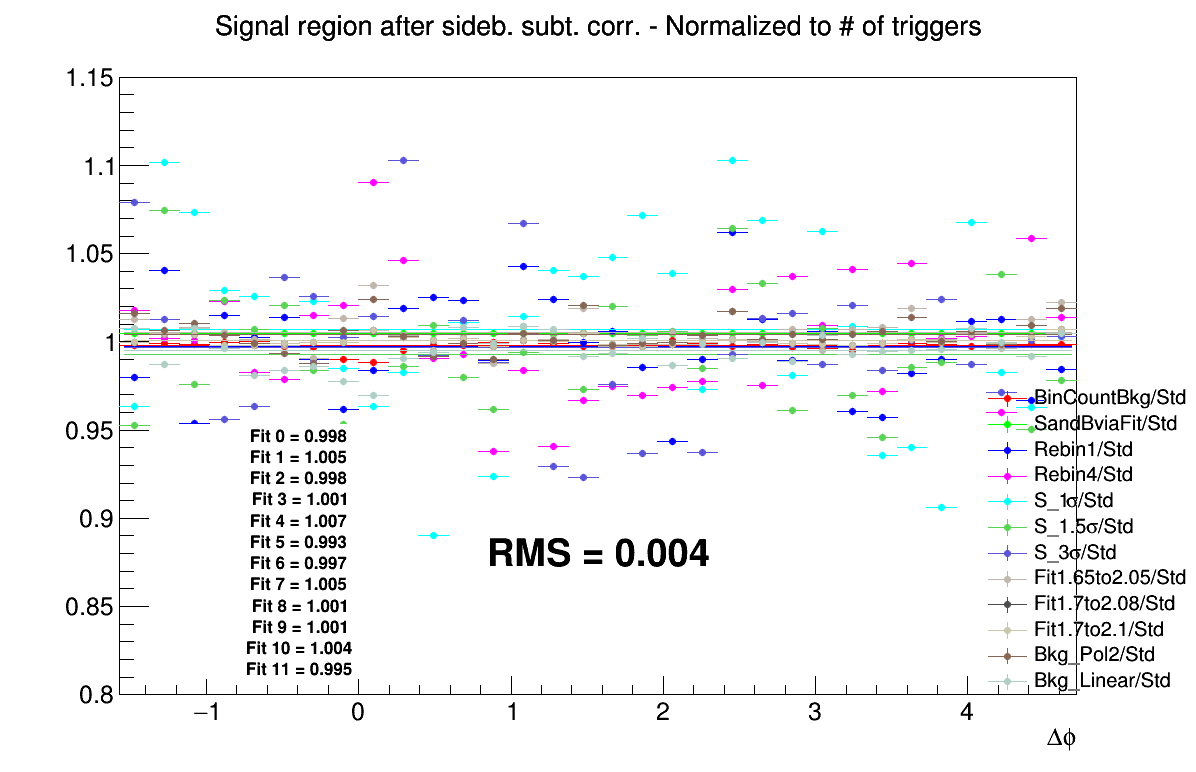
\includegraphics[width=0.31\linewidth]{figures/Systematics/Dplus/Yield/Ratio_AzimCorrDistr_Dplus_Canvas_PtIntBins8to12_PoolInt_thr1dotto99dot.png}}
{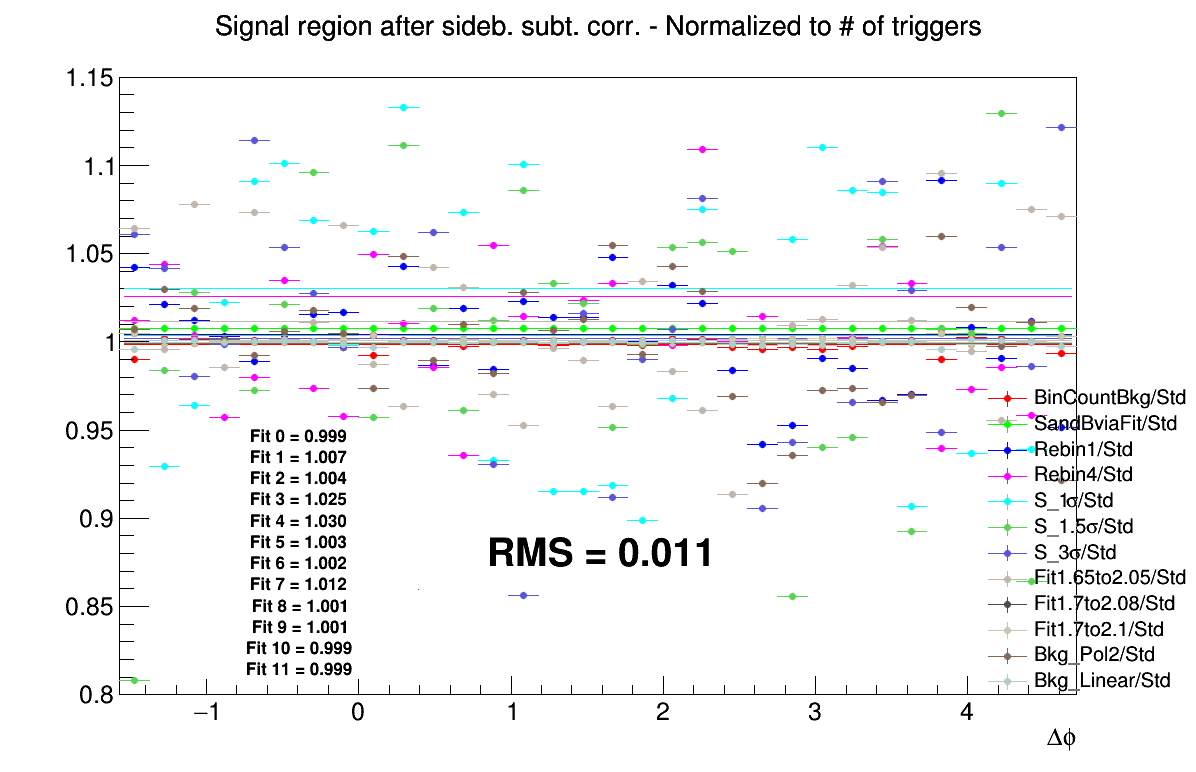
\includegraphics[width=0.31\linewidth]{figures/Systematics/Dplus/Yield/Ratio_AzimCorrDistr_Dplus_Canvas_PtIntBins13to13_PoolInt_thrdot3to1dot.png}}
{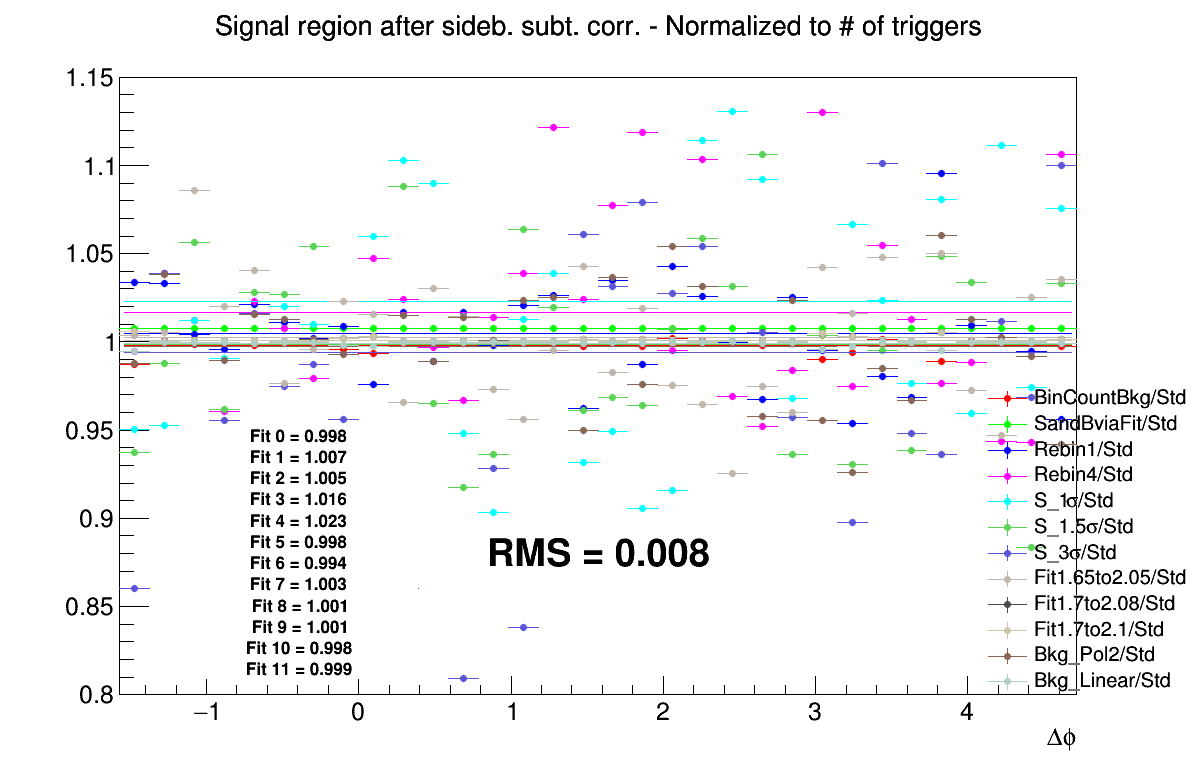
\includegraphics[width=0.31\linewidth]{figures/Systematics/Dplus/Yield/Ratio_AzimCorrDistr_Dplus_Canvas_PtIntBins13to13_PoolInt_thrdot3to99dot.png}}
{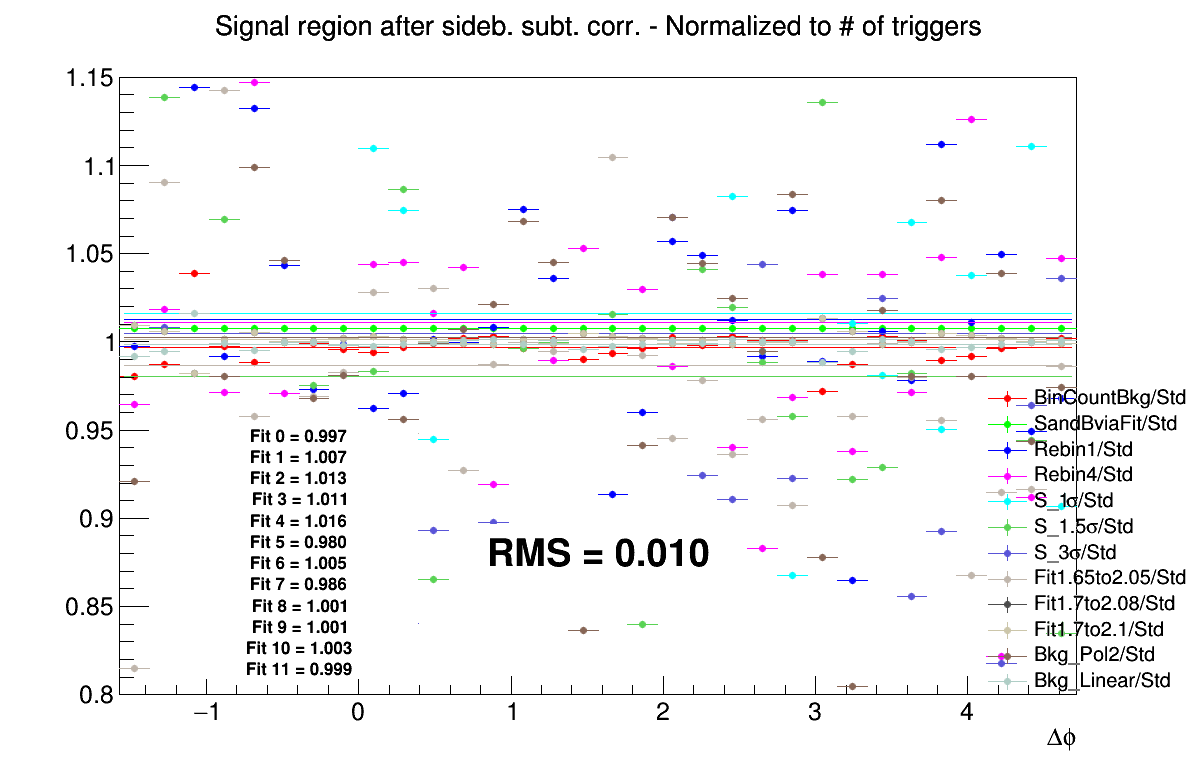
\includegraphics[width=0.31\linewidth]{figures/Systematics/Dplus/Yield/Ratio_AzimCorrDistr_Dplus_Canvas_PtIntBins13to13_PoolInt_thr1dotto99dot.png}}
\caption{Ratios of $\Dplus$-h correlation plots obtained changing S and B extraction procedure over those obtained with standard yield extraction procedure. Rows: $\pt$($\Dplus$) 3-5, 5-8, 8-16, 16-24 $\gev/c$. In each row, the panels show the associated track $\pt$ ranges 0.3-1 $\gev/c$, $>$0.3 $\gev/c$, and $>$1 $\gev/c$, respectively.}
\label{fig:Syst_DplusYield}
\end{figure}




\subsection{Uncertainty on background correlation shape}
The systematic uncertainty for the subtraction of the background correlations includes the effects due to a potentially biased description of the background correlation shape, which is evaluated from of the sidebands correlations. In particular, the background correlation shape could present some hidden invariant mass dependence. To estimate this uncertainty, the invariant mass range of the sidebands definitions was varied with respect to the default values. For the $\Dzero$ meson, the usual range of the sidebands is $4$ to $8$ $\sigma$ from the centre of the peak of the Gaussian fit and it was modified, for both sidebands to:
\begin{itemize}
    \item inner half ($4$ to $6$ $\sigma$ from the centre of the peak);
    \item outer half ($6$ to $8$ $\sigma$ from the centre of the peak)
    \item extended to $4$ to $10$ $\sigma$ (in case this is possible without exceeding the fitting range of the mass plots)
\end{itemize}

Slightly different variations, but with the same reasoning, were considered for the $\Dplus$ meson.

For the $\Dstar$ meson, the usual range of sideband in invariant mass spectra is $5$ to $10$ $\sigma$ (only on the right side) from the centre of the peak of the Gaussian fit of the invariant mass spectra,  and it was modified to:
\begin{itemize}
    \item inner half ($5$ to $8$ $\sigma$ from the centre of the peak);
    \item outer half ($8$ to $13$ $\sigma$ from the centre of the peak);
    \item extended to $5$ to $13$ $\sigma$ from the centre of the peak;
     \item extended to $6$ to $16$ $\sigma$ from the centre of the peak.
\end{itemize}

The rest of the procedure for the azimuthal correlations distribution was unchanged, and the ratios of the fully corrected azimuthal correlation plots obtained with the standard sidebands range and the correlation plots extracted with different sidebands definitions, were evaluated for each D-meson $p_\text{T}$ bin and associated tracks $p_\text{T}$ threshold. Results of this check are shown in Figures~\ref{fig:Syst_D0Bkg},~\ref{fig:Syst_DstarBkg} and~\ref{fig:Syst_DplusBkg} for $\Dzero$, $\Dstar$, $\Dplus$ respectively, for exemplary $\pt$ ranges, spanning over the full kinematic regions analysis. From the values of the ratios extracted from the checks, which do not show any azimuthal dependence a systematic uncertainty for the background subtraction can be evaluated. Also no dependence versus the associated track $\pt$ was assumed also in this case. The uncertainty was hence taken of 1-2\% for all the mesons in $3 < \pt(D) < 16$ $\gev/c$ and up to 3\% in $16 < \pt(D) < 24$ $\gev/c$.

\begin{figure}
\centering
{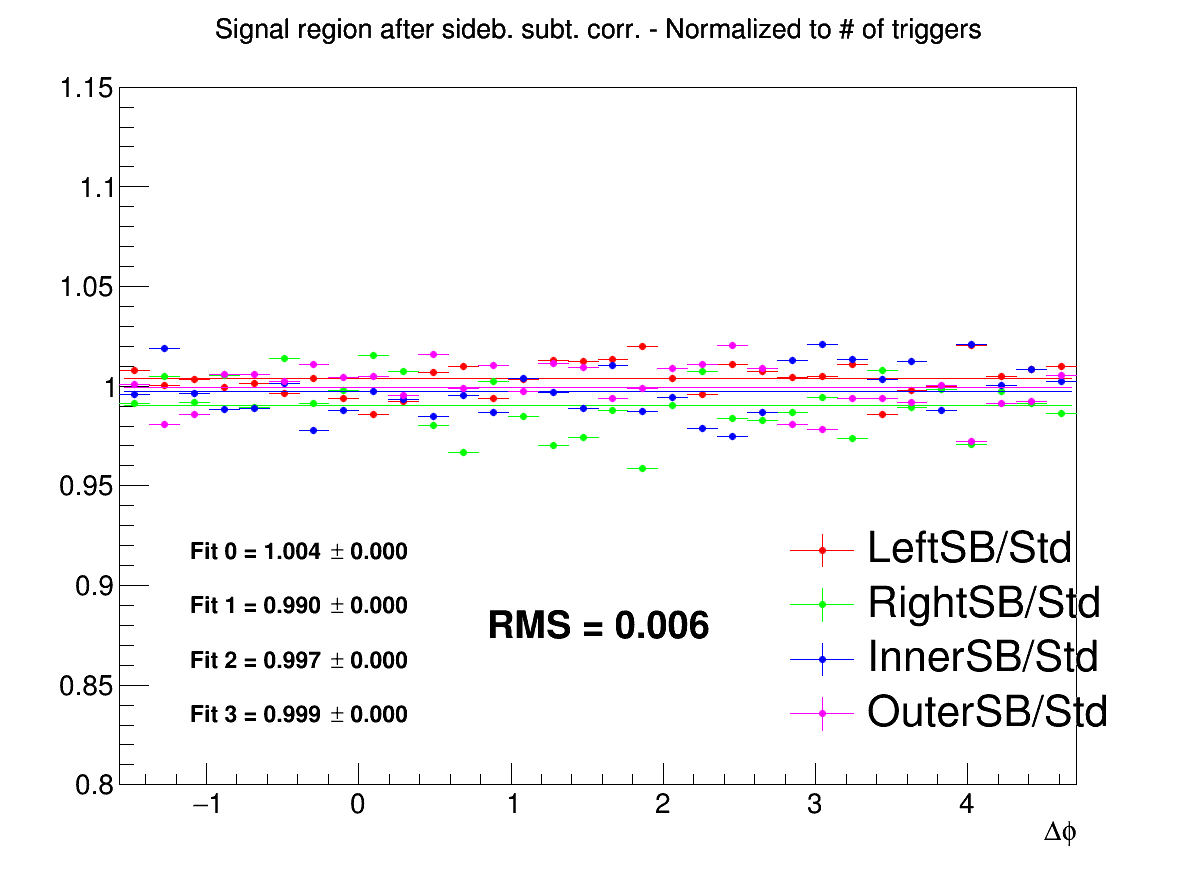
\includegraphics[width=0.31\linewidth]{figures/Systematics/Dzero/Bkg/Ratio_AzimCorrDistr_Dzero_Canvas_PtIntBins4to5_PoolInt_thr03to1.png}}
{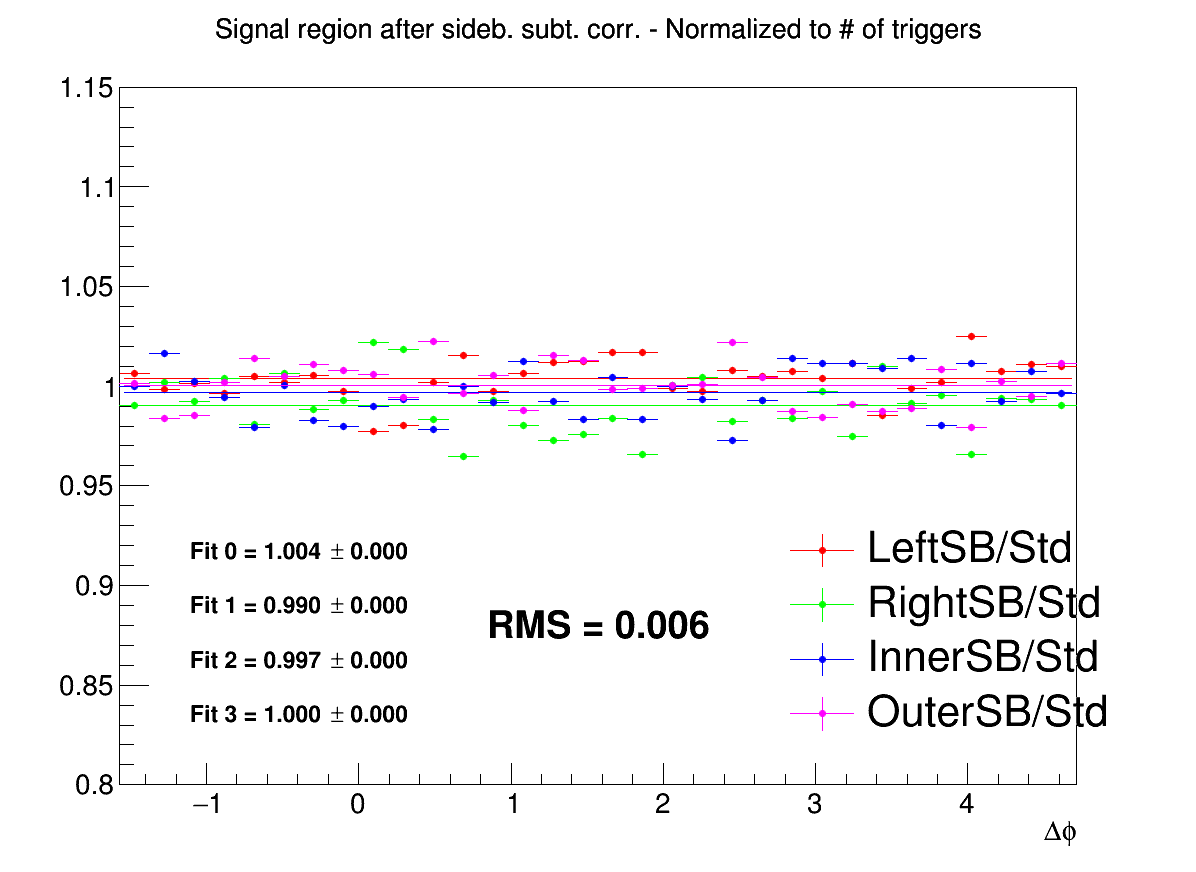
\includegraphics[width=0.31\linewidth]{figures/Systematics/Dzero/Bkg/Ratio_AzimCorrDistr_Dzero_Canvas_PtIntBins4to5_PoolInt_thr03to99.png}}
{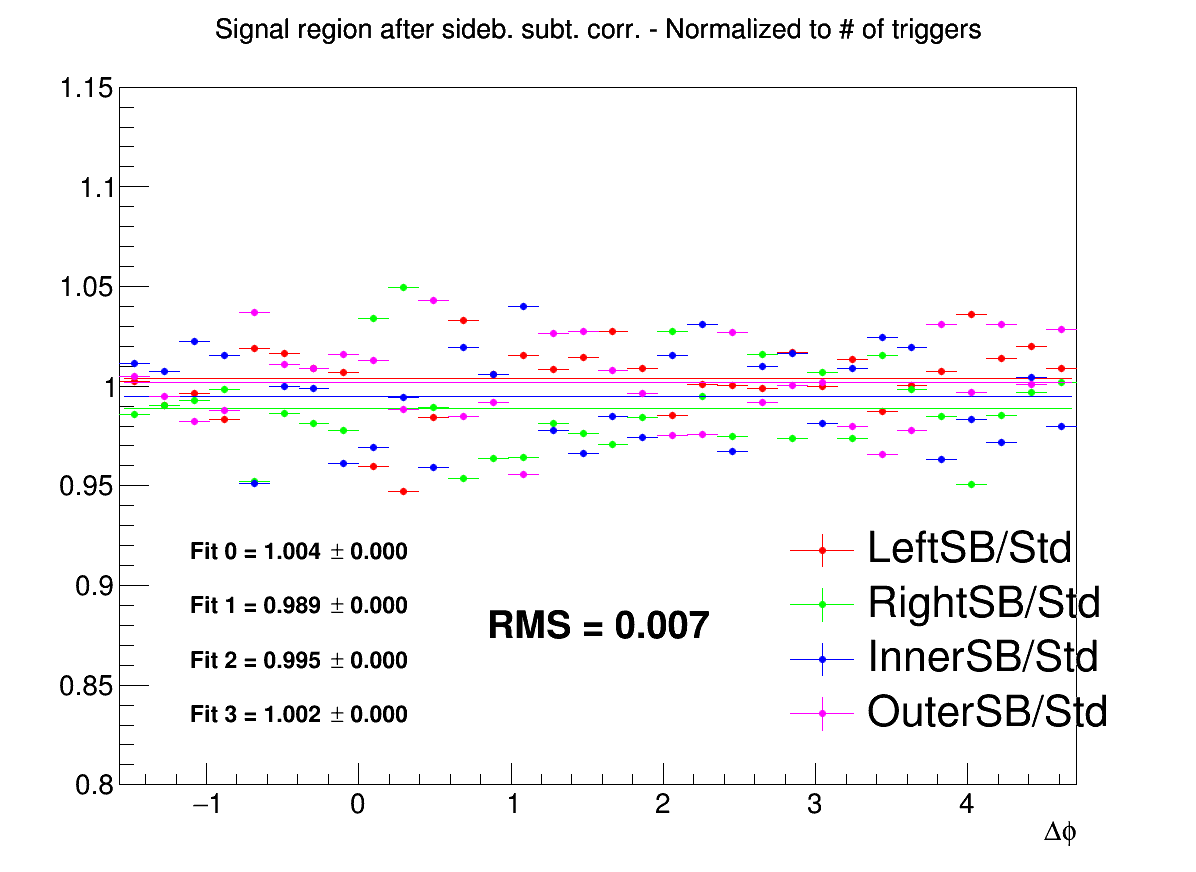
\includegraphics[width=0.31\linewidth]{figures/Systematics/Dzero/Bkg/Ratio_AzimCorrDistr_Dzero_Canvas_PtIntBins4to5_PoolInt_thr1to99.png}}
{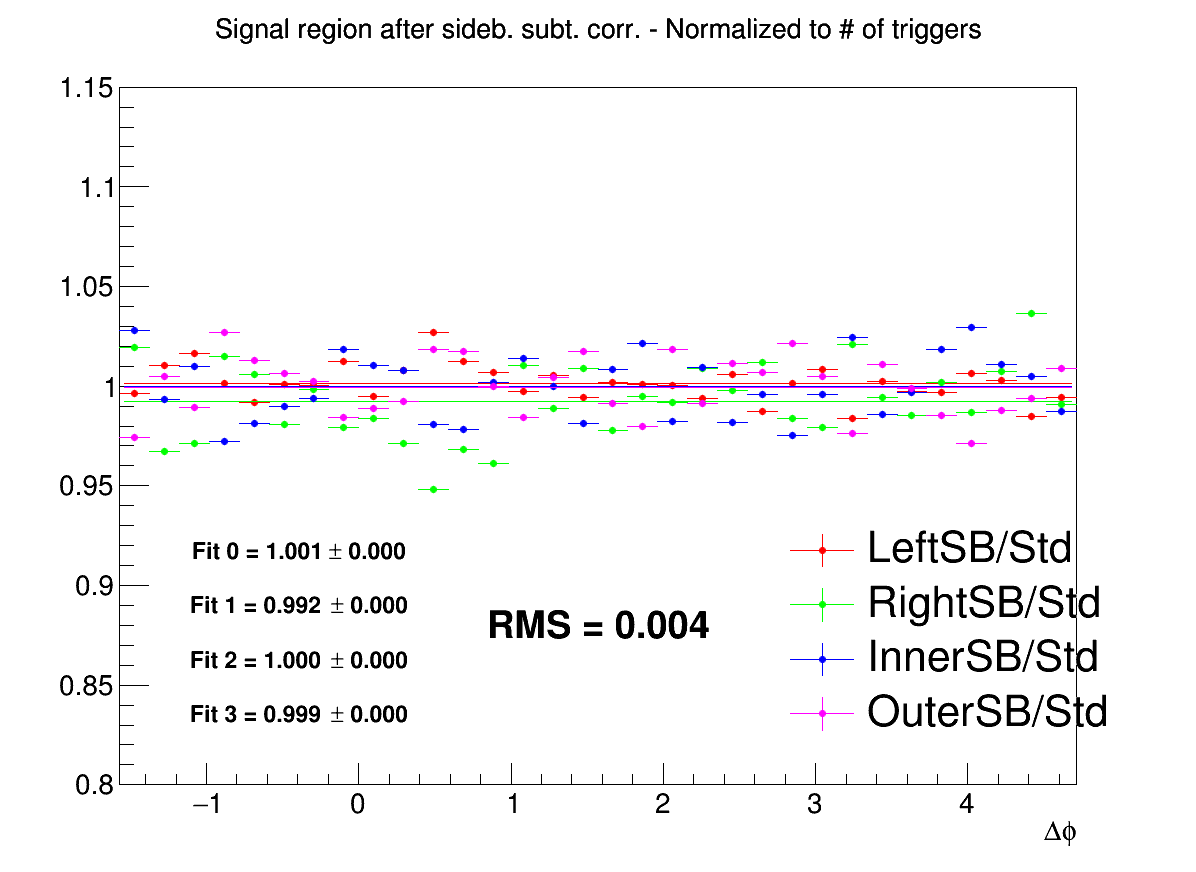
\includegraphics[width=0.31\linewidth]{figures/Systematics/Dzero/Bkg/Ratio_AzimCorrDistr_Dzero_Canvas_PtIntBins6to8_PoolInt_thr03to1.png}}
{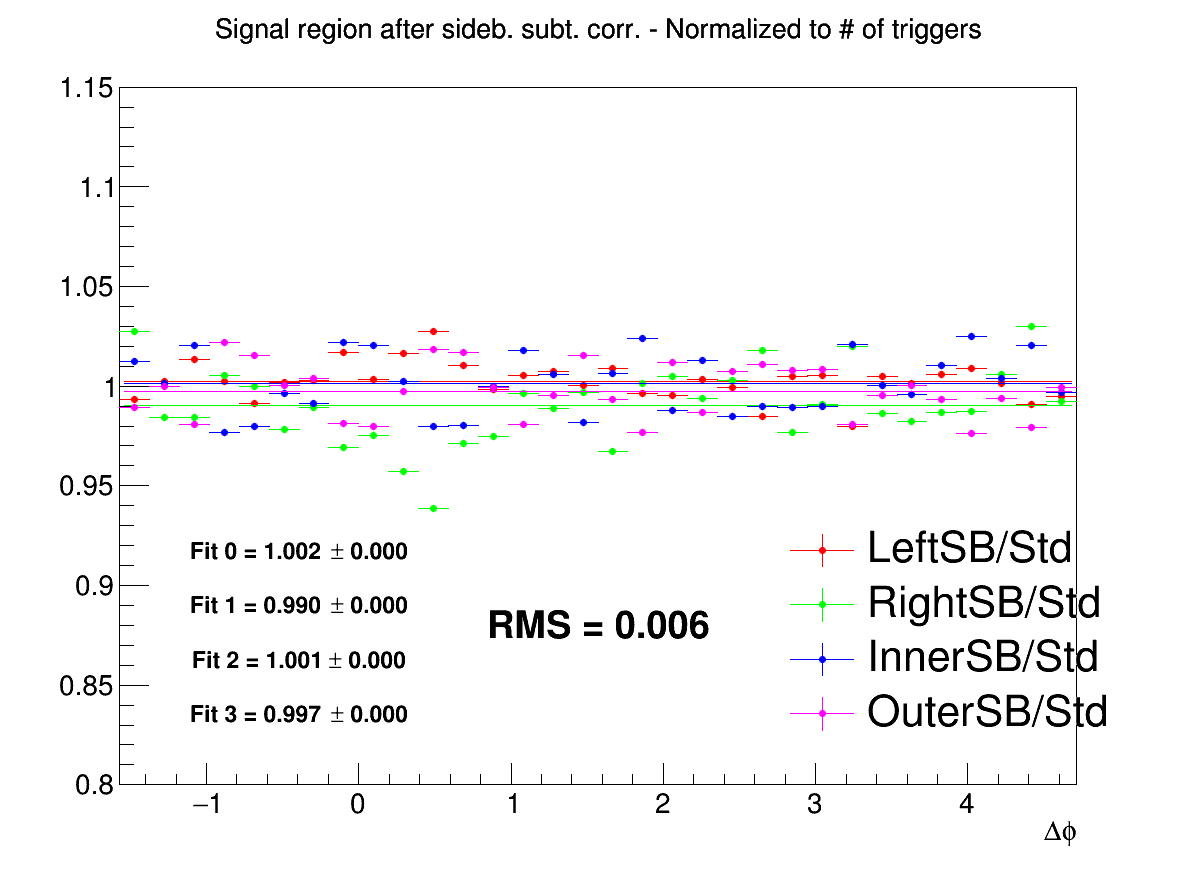
\includegraphics[width=0.31\linewidth]{figures/Systematics/Dzero/Bkg/Ratio_AzimCorrDistr_Dzero_Canvas_PtIntBins6to8_PoolInt_thr03to99.png}}
{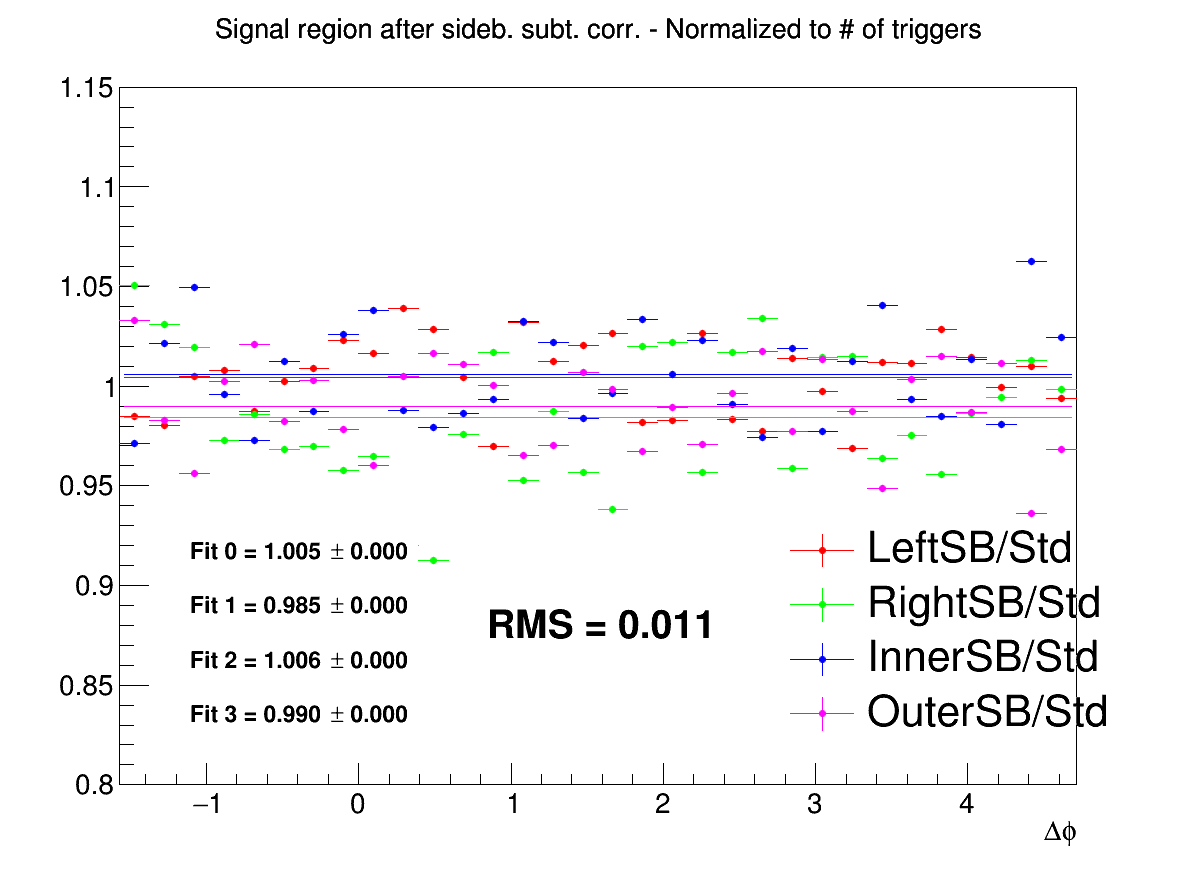
\includegraphics[width=0.31\linewidth]{figures/Systematics/Dzero/Bkg/Ratio_AzimCorrDistr_Dzero_Canvas_PtIntBins6to8_PoolInt_thr1to99.png}}
{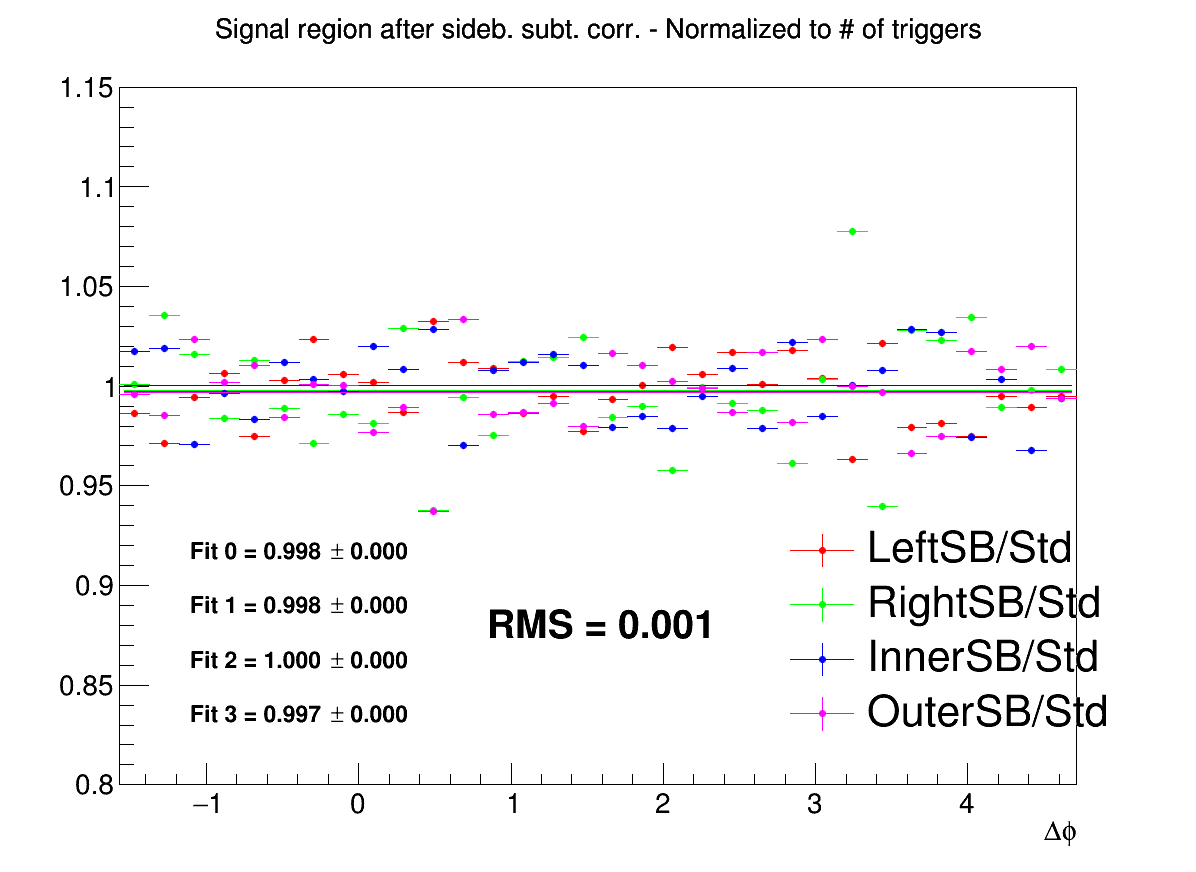
\includegraphics[width=0.31\linewidth]{figures/Systematics/Dzero/Bkg/Ratio_AzimCorrDistr_Dzero_Canvas_PtIntBins9to11_PoolInt_thr03to1.png}}
{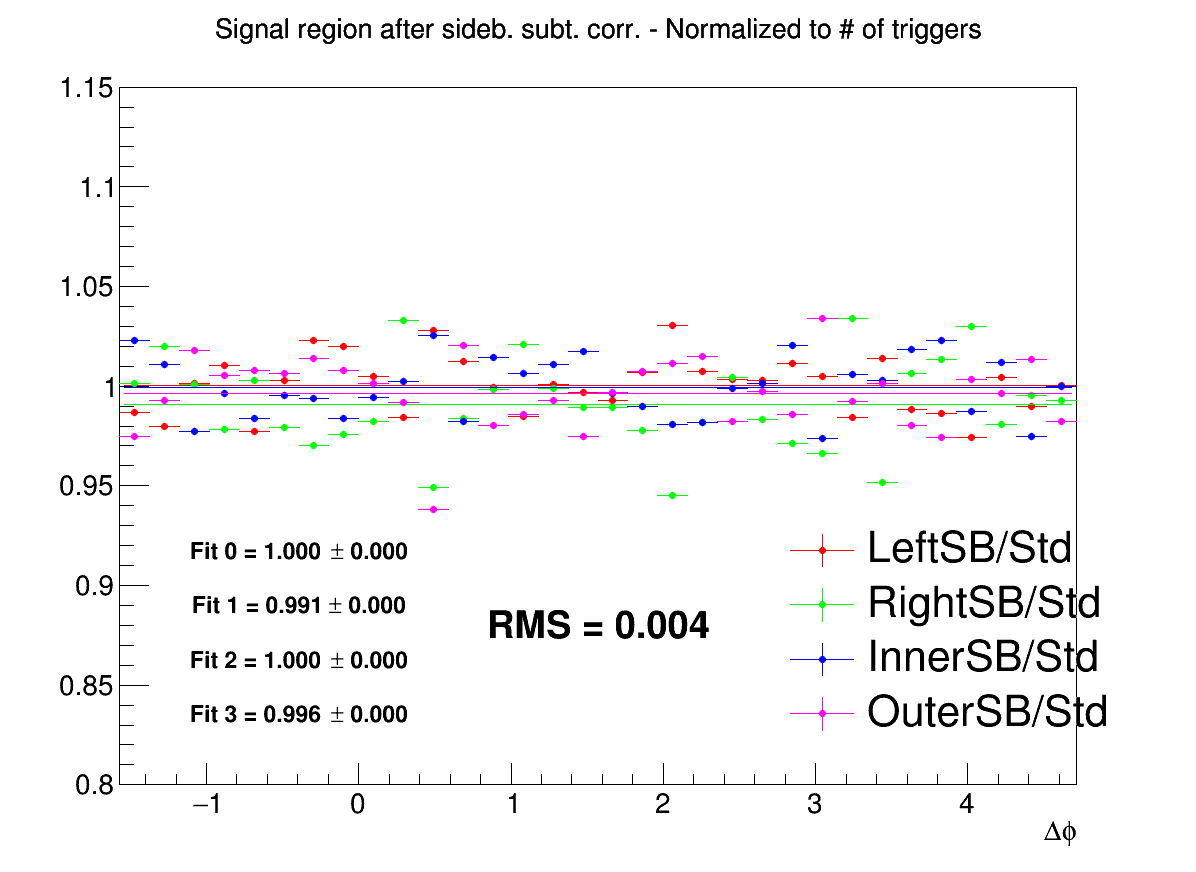
\includegraphics[width=0.31\linewidth]{figures/Systematics/Dzero/Bkg/Ratio_AzimCorrDistr_Dzero_Canvas_PtIntBins9to11_PoolInt_thr03to99.png}}
{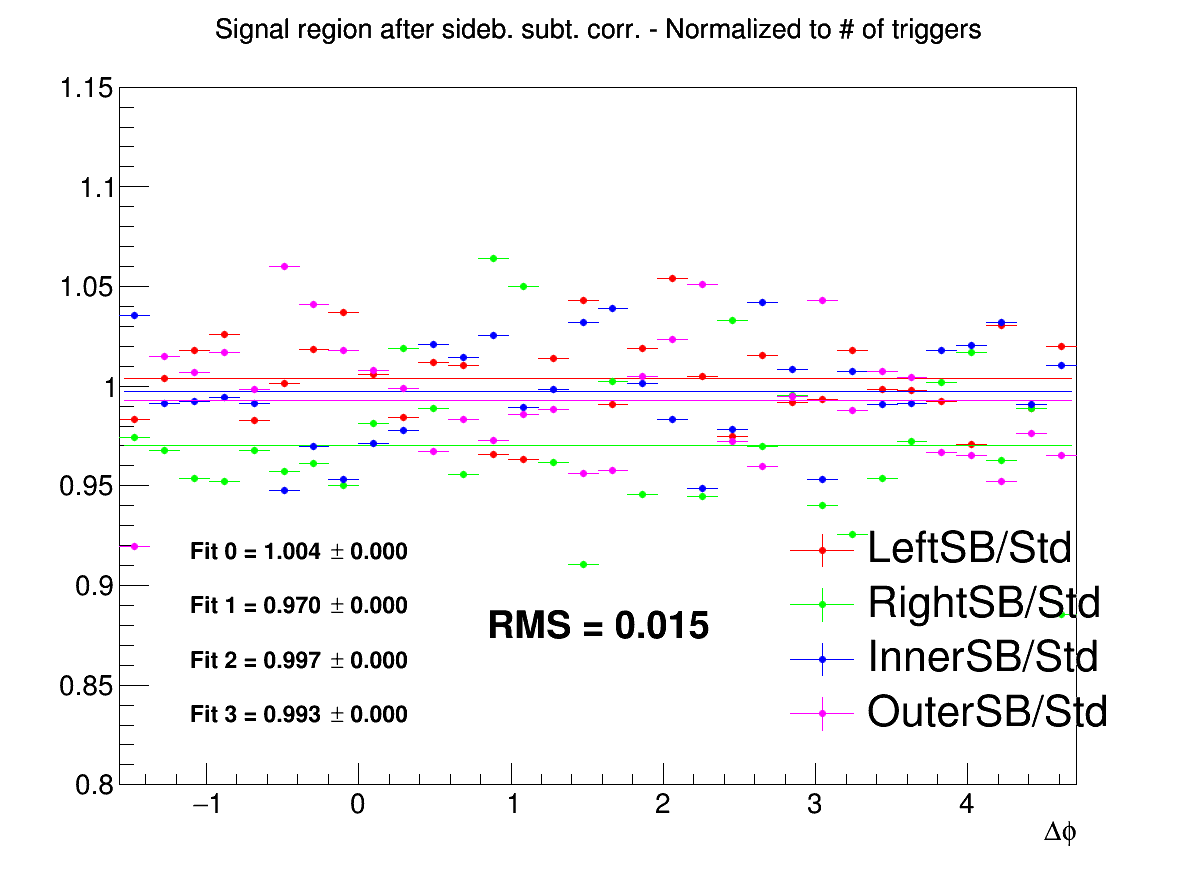
\includegraphics[width=0.31\linewidth]{figures/Systematics/Dzero/Bkg/Ratio_AzimCorrDistr_Dzero_Canvas_PtIntBins9to11_PoolInt_thr1to99.png}}
{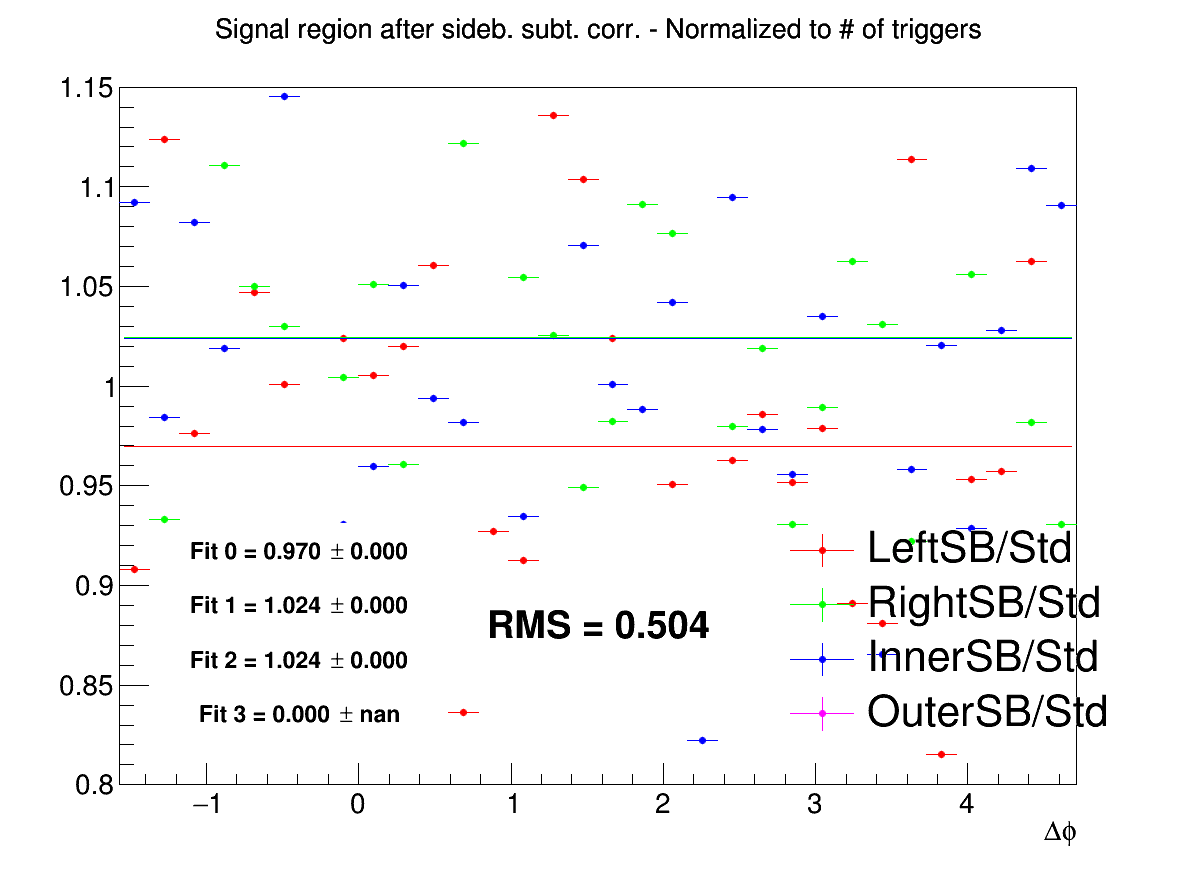
\includegraphics[width=0.31\linewidth]{figures/Systematics/Dzero/Bkg/Ratio_AzimCorrDistr_Dzero_Canvas_PtIntBins12to13_PoolInt_thr03to1.png}}
{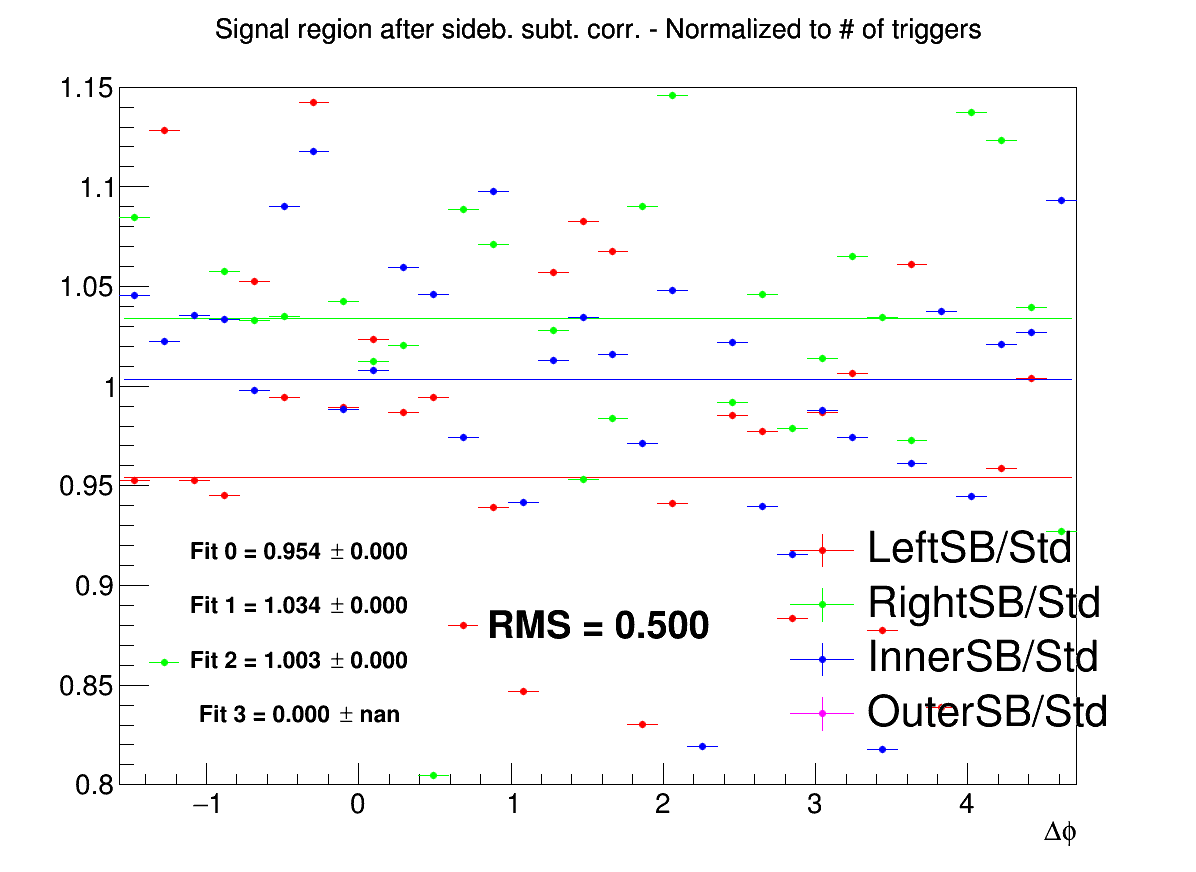
\includegraphics[width=0.31\linewidth]{figures/Systematics/Dzero/Bkg/Ratio_AzimCorrDistr_Dzero_Canvas_PtIntBins12to13_PoolInt_thr03to99.png}}
{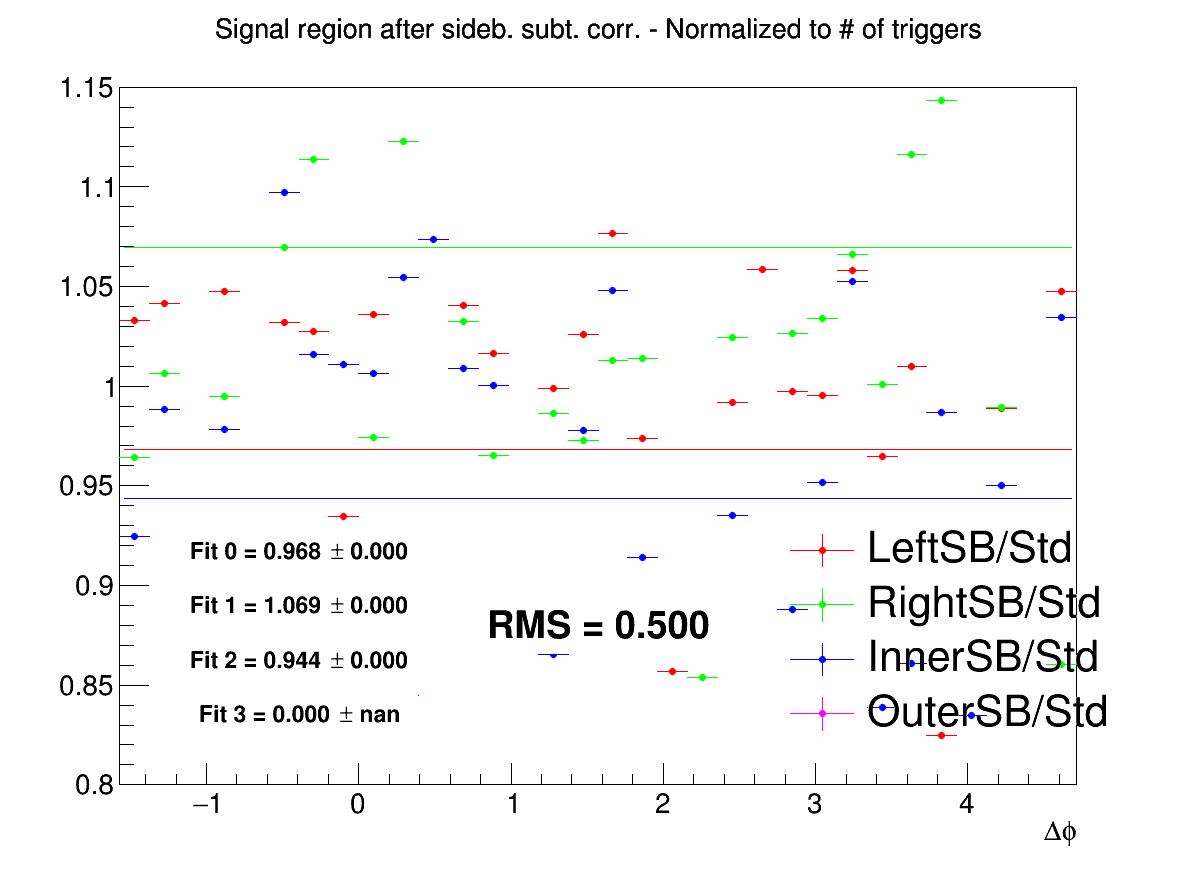
\includegraphics[width=0.31\linewidth]{figures/Systematics/Dzero/Bkg/Ratio_AzimCorrDistr_Dzero_Canvas_PtIntBins12to13_PoolInt_thr1to99.png}}
 \caption{Ratios of $\Dzero$-h correlation plots obtained by changing the sideband ranges over those obtained with standard sideband ranges. Rows: $\pt$($\Dzero$) 3-5, 5-8, 8-16, 16-24 $\gev/c$. In each row, the panels show the associated track $\pt$ ranges 0.3-1, $>$0.3 $\gev/c$ and $>$1 $\gev/c$, respectively.}
\label{fig:Syst_D0Bkg}
\end{figure}


\begin{figure}
\centering
{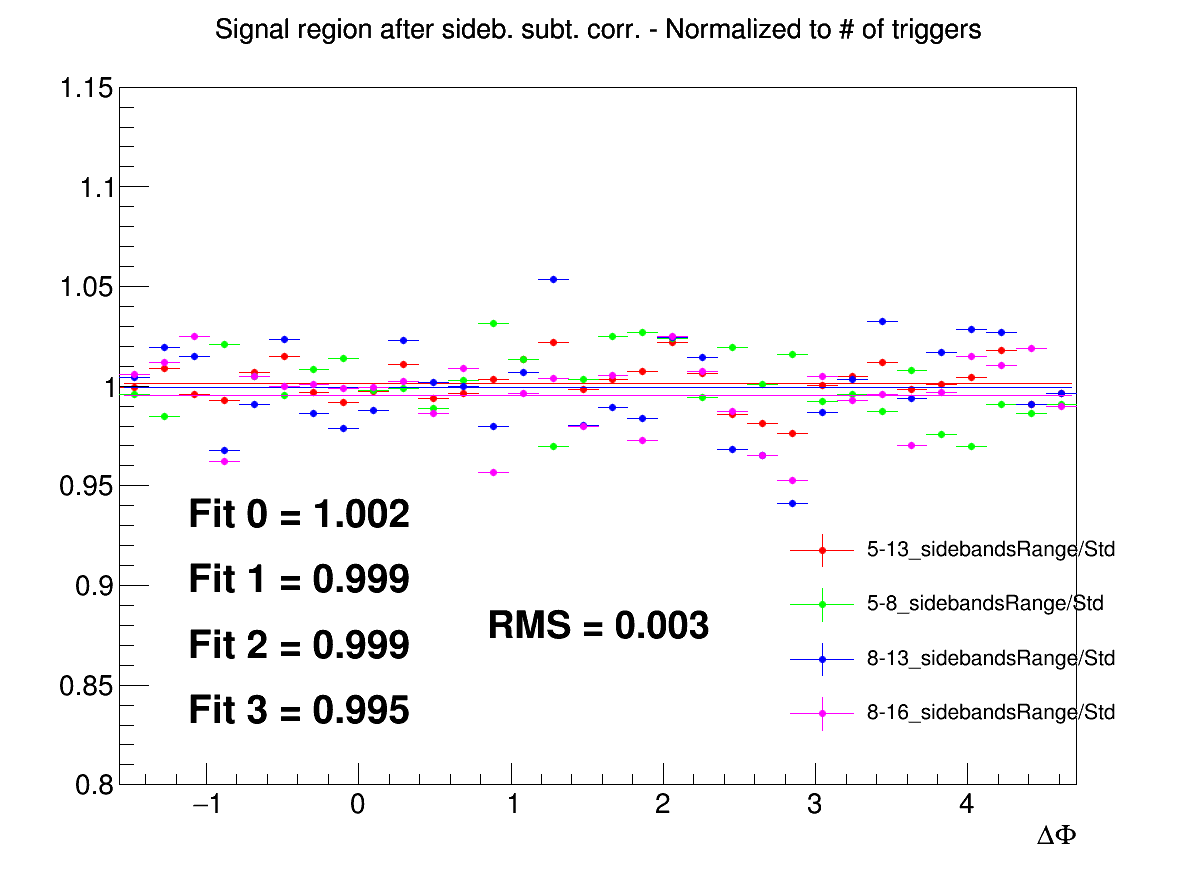
\includegraphics[width=0.31\linewidth]{figures/Systematics/Dstar/Bkg/Ratio_AzimCorrDistr_Dstar_Canvas_PtIntBins2to3_PoolInt_thrdot3to1dot_BkgShape.png}}
{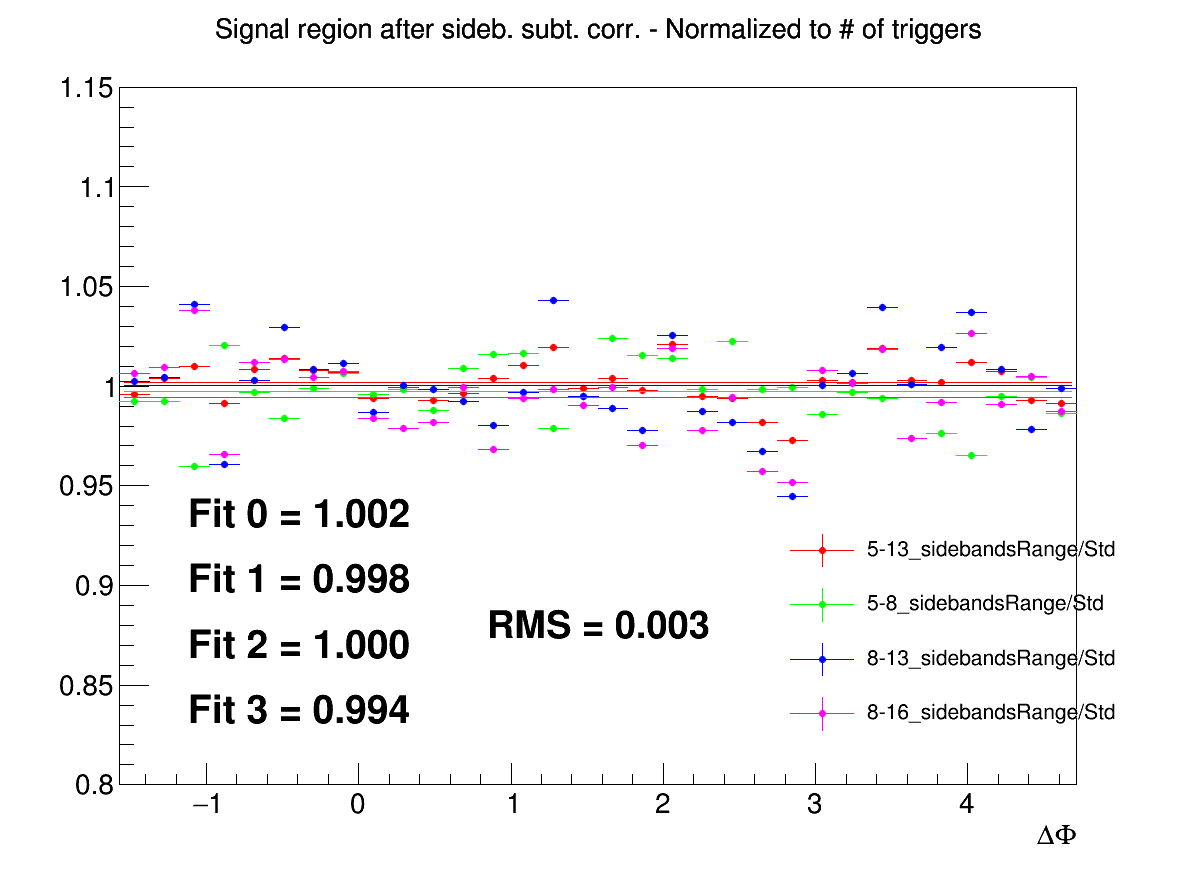
\includegraphics[width=0.31\linewidth]{figures/Systematics/Dstar/Bkg/Ratio_AzimCorrDistr_Dstar_Canvas_PtIntBins2to3_PoolInt_thrdot3to99dot_BkgShape.png}}
{\includegraphics[width=0.31\linewidth]{figures/Systematics/Dstar/Bkg/Ratio_AzimCorrDistr_Dstar_Canvas_PtIntBins2to3_PoolInt_thr1dotto99dot_BkgShape.png}}
{\includegraphics[width=0.31\linewidth]{figures/Systematics/Dstar/Bkg/Ratio_AzimCorrDistr_Dstar_Canvas_PtIntBins4to6_PoolInt_thrdot3to1dot_BkgShape.png}}
{\includegraphics[width=0.31\linewidth]{figures/Systematics/Dstar/Bkg/Ratio_AzimCorrDistr_Dstar_Canvas_PtIntBins4to6_PoolInt_thrdot3to99dot_BkgShape.png}}
{\includegraphics[width=0.31\linewidth]{figures/Systematics/Dstar/Bkg/Ratio_AzimCorrDistr_Dstar_Canvas_PtIntBins4to6_PoolInt_thr1dotto99dot_BkgShape.png}}
{\includegraphics[width=0.31\linewidth]{figures/Systematics/Dstar/Bkg/Ratio_AzimCorrDistr_Dstar_Canvas_PtIntBins7to9_PoolInt_thrdot3to1dot_BkgShape.png}}
{\includegraphics[width=0.31\linewidth]{figures/Systematics/Dstar/Bkg/Ratio_AzimCorrDistr_Dstar_Canvas_PtIntBins7to9_PoolInt_thrdot3to99dot_BkgShape.png}}
{\includegraphics[width=0.31\linewidth]{figures/Systematics/Dstar/Bkg/Ratio_AzimCorrDistr_Dstar_Canvas_PtIntBins7to9_PoolInt_thr1dotto99dot_BkgShape.png}}
{\includegraphics[width=0.31\linewidth]{figures/Systematics/Dstar/Bkg/Ratio_AzimCorrDistr_Dstar_Canvas_PtIntBins10to10_PoolInt_thrdot3to1dot_BkgShape.png}}
{\includegraphics[width=0.31\linewidth]{figures/Systematics/Dstar/Bkg/Ratio_AzimCorrDistr_Dstar_Canvas_PtIntBins10to10_PoolInt_thrdot3to99dot_BkgShape.png}}
{\includegraphics[width=0.31\linewidth]{figures/Systematics/Dstar/Bkg/Ratio_AzimCorrDistr_Dstar_Canvas_PtIntBins10to10_PoolInt_thr1dotto99dot_BkgShape.png}}

 \caption{Ratios of $\Dstar$-h correlation plots obtained by changing the sideband ranges over those obtained with standard sideband ranges. Rows: $\pt$($\Dstar$) 3-5, 5-8, 8-16, 16-24 $\gev/c$. In each row, the panels show the associated track $\pt$ ranges 0.3-1, $>$0.3 $\gev/c$ and $>$1 $\gev/c$, respectively.}
\label{fig:Syst_DstarBkg}
\end{figure}


\begin{figure}
\centering
{\includegraphics[width=0.31\linewidth]{figures/Systematics/Dplus/Bkg/Ratio_AzimCorrDistr_Dplus_Canvas_PtIntBins3to4_PoolInt_thrdot3to1dot.png}}
{\includegraphics[width=0.31\linewidth]{figures/Systematics/Dplus/Bkg/Ratio_AzimCorrDistr_Dplus_Canvas_PtIntBins3to4_PoolInt_thrdot3to99dot.png}}
{\includegraphics[width=0.31\linewidth]{figures/Systematics/Dplus/Bkg/Ratio_AzimCorrDistr_Dplus_Canvas_PtIntBins3to4_PoolInt_thr1dotto99dot.png}}
{\includegraphics[width=0.31\linewidth]{figures/Systematics/Dplus/Bkg/Ratio_AzimCorrDistr_Dplus_Canvas_PtIntBins5to7_PoolInt_thrdot3to1dot.png}}
{\includegraphics[width=0.31\linewidth]{figures/Systematics/Dplus/Bkg/Ratio_AzimCorrDistr_Dplus_Canvas_PtIntBins5to7_PoolInt_thrdot3to99dot.png}}
{\includegraphics[width=0.31\linewidth]{figures/Systematics/Dplus/Bkg/Ratio_AzimCorrDistr_Dplus_Canvas_PtIntBins5to7_PoolInt_thr1dotto99dot.png}}
{\includegraphics[width=0.31\linewidth]{figures/Systematics/Dplus/Bkg/Ratio_AzimCorrDistr_Dplus_Canvas_PtIntBins8to12_PoolInt_thrdot3to1dot.png}}
{\includegraphics[width=0.31\linewidth]{figures/Systematics/Dplus/Bkg/Ratio_AzimCorrDistr_Dplus_Canvas_PtIntBins8to12_PoolInt_thrdot3to99dot.png}}
{\includegraphics[width=0.31\linewidth]{figures/Systematics/Dplus/Bkg/Ratio_AzimCorrDistr_Dplus_Canvas_PtIntBins8to12_PoolInt_thr1dotto99dot.png}}
{\includegraphics[width=0.31\linewidth]{figures/Systematics/Dplus/Bkg/Ratio_AzimCorrDistr_Dplus_Canvas_PtIntBins13to13_PoolInt_thrdot3to1dot.png}}
{\includegraphics[width=0.31\linewidth]{figures/Systematics/Dplus/Bkg/Ratio_AzimCorrDistr_Dplus_Canvas_PtIntBins13to13_PoolInt_thrdot3to99dot.png}}
{\includegraphics[width=0.31\linewidth]{figures/Systematics/Dplus/Bkg/Ratio_AzimCorrDistr_Dplus_Canvas_PtIntBins13to13_PoolInt_thr1dotto99dot.png}}
 \caption{Ratios of $\Dplus$-h correlation plots obtained by changing the sideband ranges over those obtained with standard sideband ranges. Rows: $\pt$($\Dplus$) 3-5, 5-8, 8-16, 16-24 $\gev/c$. In each row, the panels show the associated track $\pt$ ranges 0.3-1, $>$0.3 $\gev/c$ and $>$1 $\gev/c$, respectively.}
\label{fig:Syst_DplusBkg}
\end{figure}

\subsection{Uncertainty on D-meson cut stability}
To study the systematics due to the topological selections on the D meson, the cut variation approach was used. For each D-meson, alternate sets of released and tightened selection cuts were applied to extract the correlation distribution, varying in particular the cosine of the pointing angle, the maximum DCA among the daughter tracks and the product of the daughter track impact parameters. For each set of cuts new 2D ($\pt$ vs multiplicity), D meson efficiency map was computed.
In Figures \ref{fig:D0effVars}, \ref{fig:DstareffVars}, \ref{fig:DpluseffVars} (for $\Dzero$, $\Dstar$ and $\Dplus$, respectively) the ratio of the different 1D efficiencies with the alternate cuts with respect to the default cut selection is chosen, to highlight how the different selections effectively varied the efficiency values, especially at low $\pt$, where cuts are more effective.

\begin{figure}[h]
\centering
{\includegraphics[width=.7\linewidth]{figures/Systematics/Dzero/CutVar/RatioPromptEff1DMap.png}}
\caption{Ratio of $\Dzero$ efficiencies with alternate cut variations w.r.t. the standard cut used for the analysis.}
\label{fig:D0effVars}
\end{figure}

\begin{figure}[h]
\centering
{\includegraphics[width=.7\linewidth]{figures/Systematics/Dstar/CutVar/RatioPromptEff1DMap.png}}
\caption{Ratio of $\Dstar$ efficiencies with alternate cut variations w.r.t. the standard cut used for the analysis.}
\label{fig:DstareffVars}
\end{figure}


\begin{figure}[!htbp]
\centering
{\includegraphics[width=0.70\linewidth, height=0.43\linewidth]{figures/Systematics/Dplus/Eff/EffcmpratioDplus.png}}
\caption{Ratio of $\Dplus$ efficiencies with alternate cut variations w.r.t. the standard cut used for the analysis.}
\label{fig:DpluseffVars}
\end{figure}

Figure \ref{fig:Syst_D0CutVar}, \ref{fig:Syst_DstarCutVar}, \ref{fig:Syst_DplusCutVar} show the ratio of the correlation distributions with alternate cut sets over those with the standard approach, for exemplary $\pt$ ranges covering the full kinematic region of interest for the analyses. The ratios are reasonably flat in $\Delta\varphi$, hence a flat systematic was evaluated as systematic uncertainty from D-meson the cut variations. For the $\Dzero$, the uncertainty was considered of 2\% for all the $\pt$ ranges of trigger and tracks analyzed. The uncertainty was evaluated to be from 1\% to 2.5\% depending on the D-meson specie and on the kinematic range.

\begin{figure}
\centering
{\includegraphics[width=0.31\linewidth]{figures/Systematics/Dzero/CutVar/Ratio_AzimCorrDistr_Dzero_Canvas_PtIntBins4to5_PoolInt_thr03to1.png}}
{\includegraphics[width=0.31\linewidth]{figures/Systematics/Dzero/CutVar/Ratio_AzimCorrDistr_Dzero_Canvas_PtIntBins4to5_PoolInt_thr03to99.png}}
{\includegraphics[width=0.31\linewidth]{figures/Systematics/Dzero/CutVar/Ratio_AzimCorrDistr_Dzero_Canvas_PtIntBins4to5_PoolInt_thr1to99.png}}
{\includegraphics[width=0.31\linewidth]{figures/Systematics/Dzero/CutVar/Ratio_AzimCorrDistr_Dzero_Canvas_PtIntBins6to8_PoolInt_thr03to1.png}}
{\includegraphics[width=0.31\linewidth]{figures/Systematics/Dzero/CutVar/Ratio_AzimCorrDistr_Dzero_Canvas_PtIntBins6to8_PoolInt_thr03to99.png}}
{\includegraphics[width=0.31\linewidth]{figures/Systematics/Dzero/CutVar/Ratio_AzimCorrDistr_Dzero_Canvas_PtIntBins6to8_PoolInt_thr1to99.png}}
{\includegraphics[width=0.31\linewidth]{figures/Systematics/Dzero/CutVar/Ratio_AzimCorrDistr_Dzero_Canvas_PtIntBins9to11_PoolInt_thr03to1.png}}
{\includegraphics[width=0.31\linewidth]{figures/Systematics/Dzero/CutVar/Ratio_AzimCorrDistr_Dzero_Canvas_PtIntBins9to11_PoolInt_thr03to99.png}}
{\includegraphics[width=0.31\linewidth]{figures/Systematics/Dzero/CutVar/Ratio_AzimCorrDistr_Dzero_Canvas_PtIntBins9to11_PoolInt_thr1to99.png}}
{\includegraphics[width=0.31\linewidth]{figures/Systematics/Dzero/CutVar/Ratio_AzimCorrDistr_Dzero_Canvas_PtIntBins12to13_PoolInt_thr03to1.png}}
{\includegraphics[width=0.31\linewidth]{figures/Systematics/Dzero/CutVar/Ratio_AzimCorrDistr_Dzero_Canvas_PtIntBins12to13_PoolInt_thr03to99.png}}
{\includegraphics[width=0.31\linewidth]{figures/Systematics/Dzero/CutVar/Ratio_AzimCorrDistr_Dzero_Canvas_PtIntBins12to13_PoolInt_thr1to99.png}}
 \caption{Ratios of $\Dzero$-h correlation plots obtained with alternate D-meson cut sets over those obtained with standard selection. Rows: $\pt$($\Dzero$) 3-5, 5-8, 8-16, 16-24 $\gev/c$. In each row, the panels show the associated track $\pt$ ranges 0.3-1, $>$0.3 $\gev/c$,  $>$1 $\gev/c$, respectively.}
\label{fig:Syst_D0CutVar}
\end{figure}


\begin{figure}
\centering
{\includegraphics[width=0.31\linewidth]{figures/Systematics/Dstar/CutVar/Ratio_AzimCorrDistr_Dstar_Canvas_PtIntBins2to3_PoolInt_thrdot3to1dot_CUTVar.png}}
{\includegraphics[width=0.31\linewidth]{figures/Systematics/Dstar/CutVar/Ratio_AzimCorrDistr_Dstar_Canvas_PtIntBins2to3_PoolInt_thrdot3to99dot_CUTVar.png}}
{\includegraphics[width=0.31\linewidth]{figures/Systematics/Dstar/CutVar/Ratio_AzimCorrDistr_Dstar_Canvas_PtIntBins2to3_PoolInt_thr1dotto99dot_CUTVar.png}}
{\includegraphics[width=0.31\linewidth]{figures/Systematics/Dstar/CutVar/Ratio_AzimCorrDistr_Dstar_Canvas_PtIntBins4to6_PoolInt_thrdot3to1dot_CUTVar.png}}
{\includegraphics[width=0.31\linewidth]{figures/Systematics/Dstar/CutVar/Ratio_AzimCorrDistr_Dstar_Canvas_PtIntBins4to6_PoolInt_thrdot3to99dot_CUTVar.png}}
{\includegraphics[width=0.31\linewidth]{figures/Systematics/Dstar/CutVar/Ratio_AzimCorrDistr_Dstar_Canvas_PtIntBins4to6_PoolInt_thr1dotto99dot_CUTVar.png}}
{\includegraphics[width=0.31\linewidth]{figures/Systematics/Dstar/CutVar/Ratio_AzimCorrDistr_Dstar_Canvas_PtIntBins7to9_PoolInt_thrdot3to1dot_CUTVar.png}}
{\includegraphics[width=0.31\linewidth]{figures/Systematics/Dstar/CutVar/Ratio_AzimCorrDistr_Dstar_Canvas_PtIntBins7to9_PoolInt_thrdot3to99dot_CUTVar.png}}
{\includegraphics[width=0.31\linewidth]{figures/Systematics/Dstar/CutVar/Ratio_AzimCorrDistr_Dstar_Canvas_PtIntBins7to9_PoolInt_thr1dotto99dot_CUTVar.png}}
{\includegraphics[width=0.31\linewidth]{figures/Systematics/Dstar/CutVar/Ratio_AzimCorrDistr_Dstar_Canvas_PtIntBins10to10_PoolInt_thrdot3to1dot_CUTVar.png}}
{\includegraphics[width=0.31\linewidth]{figures/Systematics/Dstar/CutVar/Ratio_AzimCorrDistr_Dstar_Canvas_PtIntBins10to10_PoolInt_thrdot3to99dot_CUTVar.png}}
{\includegraphics[width=0.31\linewidth]{figures/Systematics/Dstar/CutVar/Ratio_AzimCorrDistr_Dstar_Canvas_PtIntBins10to10_PoolInt_thr1dotto99dot_CUTVar.png}}

 \caption{Ratios of $\Dstar$-h correlation plots obtained with alternate D-meson cut sets over those obtained with standard selection. Rows: $\pt$($\Dstar$) 3-5, 5-8, 8-16, 16-24 $\gev/c$. In each row, the panels show the associated track $\pt$ ranges 0.3-1, $>$0.3 $\gev/c$,  $>$1 $\gev/c$, respectively.}
\label{fig:Syst_DstarCutVar}
\end{figure}


\begin{figure}
\centering
{\includegraphics[width=0.31\linewidth]{figures/Systematics/Dplus/CutVar/Ratio_AzimCorrDistr_Dplus_Canvas_PtIntBins3to4_PoolInt_thrdot3to1dot.png}}
{\includegraphics[width=0.31\linewidth]{figures/Systematics/Dplus/CutVar/Ratio_AzimCorrDistr_Dplus_Canvas_PtIntBins3to4_PoolInt_thrdot3to99dot.png}}
{\includegraphics[width=0.31\linewidth]{figures/Systematics/Dplus/CutVar/Ratio_AzimCorrDistr_Dplus_Canvas_PtIntBins3to4_PoolInt_thr1dotto99dot.png}}
{\includegraphics[width=0.31\linewidth]{figures/Systematics/Dplus/CutVar/Ratio_AzimCorrDistr_Dplus_Canvas_PtIntBins5to7_PoolInt_thrdot3to1dot.png}}
{\includegraphics[width=0.31\linewidth]{figures/Systematics/Dplus/CutVar/Ratio_AzimCorrDistr_Dplus_Canvas_PtIntBins5to7_PoolInt_thrdot3to99dot.png}}
{\includegraphics[width=0.31\linewidth]{figures/Systematics/Dplus/CutVar/Ratio_AzimCorrDistr_Dplus_Canvas_PtIntBins5to7_PoolInt_thr1dotto99dot.png}}
{\includegraphics[width=0.31\linewidth]{figures/Systematics/Dplus/CutVar/Ratio_AzimCorrDistr_Dplus_Canvas_PtIntBins8to12_PoolInt_thrdot3to1dot.png}}
{\includegraphics[width=0.31\linewidth]{figures/Systematics/Dplus/CutVar/Ratio_AzimCorrDistr_Dplus_Canvas_PtIntBins8to12_PoolInt_thrdot3to99dot.png}}
{\includegraphics[width=0.31\linewidth]{figures/Systematics/Dplus/CutVar/Ratio_AzimCorrDistr_Dplus_Canvas_PtIntBins8to12_PoolInt_thr1dotto99dot.png}}
{\includegraphics[width=0.31\linewidth]{figures/Systematics/Dplus/CutVar/Ratio_AzimCorrDistr_Dplus_Canvas_PtIntBins13to13_PoolInt_thrdot3to1dot.png}}
{\includegraphics[width=0.31\linewidth]{figures/Systematics/Dplus/CutVar/Ratio_AzimCorrDistr_Dplus_Canvas_PtIntBins13to13_PoolInt_thrdot3to99dot.png}}
{\includegraphics[width=0.31\linewidth]{figures/Systematics/Dplus/CutVar/Ratio_AzimCorrDistr_Dplus_Canvas_PtIntBins13to13_PoolInt_thr1dotto99dot.png}}
 \caption{Ratios of $\Dplus$-h correlation plots obtained with alternate D-meson cut sets over those obtained with standard selection. Rows: $\pt$($\Dplus$) 3-5, 5-8, 8-16, 16-24 $\gev/c$. In each row, the panels show the associated track $\pt$ ranges 0.3-1, $>$0.3 $\gev/c$,  $>$1 $\gev/c$, respectively.}
\label{fig:Syst_DplusCutVar}
\end{figure}

\clearpage
\subsection{Uncertainty on tracking efficiency evaluation}
The systematic uncertainty assigned to cover a possible bias on the associated tracking efficiency is evaluated by varying the associated track selection.
With respect to what done in subsection 4.4, additional variations were studied, for all the D-mesons, in particular:
\begin{itemize}
  \item No request on the minimum number of ITS clusters
  \item Minimum 3 ITS clusters + kAny request for SPD + filterbit 4 request
  \item Minimum number of TPC crossed row or 90
  \item Minimum ratio of TPC crossed rows/findable crossed rows of 0.9
  \item $\pt$-dependent cut on minimum number of TPC clusters ($> 120-(5/\pt)$)
\end{itemize}

Figures \ref{fig:TrEffVariations} show the associated track selection and reconstruction efficiencies (and their ratios w.r.t. standard-cut efficiency) for alternate cut sets.

\begin{figure}
\centering
{\includegraphics[width=0.75\linewidth]{figures/Systematics/Dzero/TrackCut/AltTrackEff.png}}
\caption{Associated track selection and reconstruction efficiencies for alternate selections.}
\label{fig:TrEffVariations}
\end{figure}

In Fig. \ref{fig:SysTrEff}, \ref{fig:SysTrEff_Dstar}, \ref{fig:SysTrEff_Dplus} the ratios of correlation distributions with alternate/standard track selections are shown, in the various $\pt$ ranges, for the $\Dzero$, $\Dstar$ and $\Dplus$ mesons as trigger, respectively.
For this uncertainty, to the values obtained from the above ratio an additional 2\%, for a wrong evaluation of the ITS-TPC matching efficiency, is added in quadrature, as prescribed by the DPG group (being 1\% for associated track $\pt <$ 1, 2\% in 1-2 and 2.7\% in 2-3 $\gevc$).
The assigned uncertainty is 3 to 4.5\%, slightly increasing with the $\pt$ of the associated tracks (mainly due to the increase of the ITS-TPC matching efficiency).

\begin{figure}
\centering
{\includegraphics[width=0.31\linewidth]{figures/Systematics/Dzero/TrackCut/Ratio_AzimCorrDistr_Dzero_Canvas_PtIntBins4to5_PoolInt_thr03to99.png}}
{\includegraphics[width=0.31\linewidth]{figures/Systematics/Dzero/TrackCut/Ratio_AzimCorrDistr_Dzero_Canvas_PtIntBins4to5_PoolInt_thr03to1.png}}
{\includegraphics[width=0.31\linewidth]{figures/Systematics/Dzero/TrackCut/Ratio_AzimCorrDistr_Dzero_Canvas_PtIntBins4to5_PoolInt_thr1to99.png}} \\
{\includegraphics[width=0.31\linewidth]{figures/Systematics/Dzero/TrackCut/Ratio_AzimCorrDistr_Dzero_Canvas_PtIntBins6to8_PoolInt_thr03to99.png}}
{\includegraphics[width=0.31\linewidth]{figures/Systematics/Dzero/TrackCut/Ratio_AzimCorrDistr_Dzero_Canvas_PtIntBins6to8_PoolInt_thr03to1.png}}
{\includegraphics[width=0.31\linewidth]{figures/Systematics/Dzero/TrackCut/Ratio_AzimCorrDistr_Dzero_Canvas_PtIntBins6to8_PoolInt_thr1to99.png}} \\
{\includegraphics[width=0.31\linewidth]{figures/Systematics/Dzero/TrackCut/Ratio_AzimCorrDistr_Dzero_Canvas_PtIntBins9to11_PoolInt_thr03to99.png}}
{\includegraphics[width=0.31\linewidth]{figures/Systematics/Dzero/TrackCut/Ratio_AzimCorrDistr_Dzero_Canvas_PtIntBins9to11_PoolInt_thr03to1.png}}
{\includegraphics[width=0.31\linewidth]{figures/Systematics/Dzero/TrackCut/Ratio_AzimCorrDistr_Dzero_Canvas_PtIntBins9to11_PoolInt_thr1to99.png}} \\
{\includegraphics[width=0.31\linewidth]{figures/Systematics/Dzero/TrackCut/Ratio_AzimCorrDistr_Dzero_Canvas_PtIntBins12to13_PoolInt_thr03to99.png}}
{\includegraphics[width=0.31\linewidth]{figures/Systematics/Dzero/TrackCut/Ratio_AzimCorrDistr_Dzero_Canvas_PtIntBins12to13_PoolInt_thr03to1.png}}
{\includegraphics[width=0.31\linewidth]{figures/Systematics/Dzero/TrackCut/Ratio_AzimCorrDistr_Dzero_Canvas_PtIntBins12to13_PoolInt_thr1to99.png}} \\
 \caption{Ratios of $\Dzero$-h correlation plots obtained with alternate associated track selection over those obtained with the standard cuts. Rows: $\pt$($\Dzero$) 3-5, 5-8, 8-16, 16-24 GeV/$c$. In each row, the panels show the associated track
$\pt$ ranges $> 0.3$, 0.3-1, $> 1$ GeV/$c$, respectively.}
\label{fig:SysTrEff}
\end{figure}


\begin{figure}
\centering
{\includegraphics[width=0.31\linewidth]{figures/Systematics/Dplus/TrackCut/Ratio_AzimCorrDistr_Dplus_Canvas_PtIntBins3to4_PoolInt_thrdot3to99dot.png}}
{\includegraphics[width=0.31\linewidth]{figures/Systematics/Dplus/TrackCut/Ratio_AzimCorrDistr_Dplus_Canvas_PtIntBins3to4_PoolInt_thrdot3to1dot.png}}
{\includegraphics[width=0.31\linewidth]{figures/Systematics/Dplus/TrackCut/Ratio_AzimCorrDistr_Dplus_Canvas_PtIntBins3to4_PoolInt_thr1dotto99dot.png}} \\
{\includegraphics[width=0.31\linewidth]{figures/Systematics/Dplus/TrackCut/Ratio_AzimCorrDistr_Dplus_Canvas_PtIntBins5to7_PoolInt_thrdot3to99dot.png}}
{\includegraphics[width=0.31\linewidth]{figures/Systematics/Dplus/TrackCut/Ratio_AzimCorrDistr_Dplus_Canvas_PtIntBins5to7_PoolInt_thrdot3to1dot.png}}
{\includegraphics[width=0.31\linewidth]{figures/Systematics/Dplus/TrackCut/Ratio_AzimCorrDistr_Dplus_Canvas_PtIntBins5to7_PoolInt_thr1dotto99dot.png}} \\
{\includegraphics[width=0.31\linewidth]{figures/Systematics/Dplus/TrackCut/Ratio_AzimCorrDistr_Dplus_Canvas_PtIntBins8to12_PoolInt_thrdot3to99dot.png}}
{\includegraphics[width=0.31\linewidth]{figures/Systematics/Dplus/TrackCut/Ratio_AzimCorrDistr_Dplus_Canvas_PtIntBins8to12_PoolInt_thrdot3to1dot.png}}
{\includegraphics[width=0.31\linewidth]{figures/Systematics/Dplus/TrackCut/Ratio_AzimCorrDistr_Dplus_Canvas_PtIntBins8to12_PoolInt_thr1dotto99dot.png}} \\
{\includegraphics[width=0.31\linewidth]{figures/Systematics/Dplus/TrackCut/Ratio_AzimCorrDistr_Dplus_Canvas_PtIntBins13to13_PoolInt_thrdot3to99dot.png}}
{\includegraphics[width=0.31\linewidth]{figures/Systematics/Dplus/TrackCut/Ratio_AzimCorrDistr_Dplus_Canvas_PtIntBins13to13_PoolInt_thrdot3to1dot.png}}
{\includegraphics[width=0.31\linewidth]{figures/Systematics/Dplus/TrackCut/Ratio_AzimCorrDistr_Dplus_Canvas_PtIntBins13to13_PoolInt_thr1dotto99dot.png}} \\
 \caption{Ratios of $\Dplus$-h correlation plots obtained with alternate associated track selection over those obtained with the standard cuts. Rows: $\pt$($\Dplus$) 3-5, 5-8, 8-16, 16-24 GeV/$c$. In each row, the panels show the associated track
$\pt$ ranges $> 0.3$, 0.3-1, $> 1$ GeV/$c$, respectively.}
\label{fig:SysTrEff_Dplus}
\end{figure}

\begin{figure}
\centering
{\includegraphics[width=0.31\linewidth]{figures/Systematics/Dstar/TrkEff/Ratio_AzimCorrDistr_Dstar_Canvas_PtIntBins2to3_PoolInt_thrdot3to1dot_TrkEff.png}}
{\includegraphics[width=0.31\linewidth]{figures/Systematics/Dstar/TrkEff/Ratio_AzimCorrDistr_Dstar_Canvas_PtIntBins2to3_PoolInt_thrdot3to99dot_TrkEff.png}}
{\includegraphics[width=0.31\linewidth]{figures/Systematics/Dstar/TrkEff/Ratio_AzimCorrDistr_Dstar_Canvas_PtIntBins2to3_PoolInt_thr1dotto99dot_TrkEff.png}}
{\includegraphics[width=0.31\linewidth]{figures/Systematics/Dstar/TrkEff/Ratio_AzimCorrDistr_Dstar_Canvas_PtIntBins4to6_PoolInt_thrdot3to1dot_TrkEff.png}}
{\includegraphics[width=0.31\linewidth]{figures/Systematics/Dstar/TrkEff/Ratio_AzimCorrDistr_Dstar_Canvas_PtIntBins4to6_PoolInt_thrdot3to99dot_TrkEff.png}}
{\includegraphics[width=0.31\linewidth]{figures/Systematics/Dstar/TrkEff/Ratio_AzimCorrDistr_Dstar_Canvas_PtIntBins4to6_PoolInt_thr1dotto99dot_TrkEff.png}}
{\includegraphics[width=0.31\linewidth]{figures/Systematics/Dstar/TrkEff/Ratio_AzimCorrDistr_Dstar_Canvas_PtIntBins7to9_PoolInt_thrdot3to1dot_TrkEff.png}}
{\includegraphics[width=0.31\linewidth]{figures/Systematics/Dstar/TrkEff/Ratio_AzimCorrDistr_Dstar_Canvas_PtIntBins7to9_PoolInt_thrdot3to99dot_TrkEff.png}}
{\includegraphics[width=0.31\linewidth]{figures/Systematics/Dstar/TrkEff/Ratio_AzimCorrDistr_Dstar_Canvas_PtIntBins7to9_PoolInt_thr1dotto99dot_TrkEff.png}}
{\includegraphics[width=0.31\linewidth]{figures/Systematics/Dstar/TrkEff/Ratio_AzimCorrDistr_Dstar_Canvas_PtIntBins10to10_PoolInt_thrdot3to1dot_TrkEff.png}}
{\includegraphics[width=0.31\linewidth]{figures/Systematics/Dstar/TrkEff/Ratio_AzimCorrDistr_Dstar_Canvas_PtIntBins10to10_PoolInt_thrdot3to99dot_TrkEff.png}}
{\includegraphics[width=0.31\linewidth]{figures/Systematics/Dstar/TrkEff/Ratio_AzimCorrDistr_Dstar_Canvas_PtIntBins10to10_PoolInt_thr1dotto99dot_TrkEff.png}}\\
 \caption{Ratios of $\Dstar$-h correlation plots obtained with alternate associated track selection over those obtained with the standard cuts. Rows: $\pt$($\Dstar$) 3-5, 5-8, 8-16, 16-24 GeV/$c$. In each row, the panels show the associated track
$\pt$ ranges $> 0.3$, 0.3-1, $> 1$ GeV/$c$, respectively.}
\label{fig:SysTrEff_Dstar}
\end{figure}

\subsection{Uncertainty on secondary particle contamination}
Secondary particles, i.e. particles coming from strange hadrons decays or particles produced in interactions with the material, are expected to be tagged and removed by means of a distance of closest approach (DCA) from primary vertex cut. The uncertainty arising from the residual contamination of secondary tracks can be estimated from a Monte Carlo study, at reconstructed level. The number of primary/secondary tracks which are accepted/rejected from the DCA cut was determined for different values of the DCA selection, and the correlation distributions for the various cases were evaluated. The variations were done in the $xy$ direction, where the DCA resolution is better, and the following cases were tried (in addition to the default 1 cm cut): 0.1 cm, 0.25 cm, 0.5 cm, filtering DCA cut (i.e. 2.4 cm).

Figure~\ref{fig:DCAvar} shows the amount of secondary tracks which are accepted by the DCA cut, over the total number of tracks (primary and secondary) accepted by the selection, for the various DCA selections that were tried. This is shown for the exemplary case of $5 < \pt < 8$ $\gev/c$ (there's no $\pt$(D) dependence) and as a function of the associated track $\pt$ ranges. Hence, this quantity represents the residual contamination of secondary tracks in our reconstructed track sample. From these values, the corresponding primary track purities (1-contamination) were extracted, in each of the momentum ranges.
It was also verified that, for all the cut selections, the $\Delta\varphi$ distributions of the residual contaminations were rather flattish (anyway, a bin-by-bin dependent purity correction value was evaluated, as for the standard analysis).

\begin{figure}[h]
\centering
\resizebox{0.47\textwidth}{!}{\includegraphics[width=.47\linewidth]{figures/Systematics/Common/Purity/FractOfSecOverTotal_5to8_240.png}}
\resizebox{0.47\textwidth}{!}{\includegraphics[width=.47\linewidth]{figures/Systematics/Common/Purity/FractOfSecOverTotal_5to8_100.png}} \\
\resizebox{0.47\textwidth}{!}{\includegraphics[width=.47\linewidth]{figures/Systematics/Common/Purity/FractOfSecOverTotal_5to8_050.png}}
\resizebox{0.47\textwidth}{!}{\includegraphics[width=.47\linewidth]{figures/Systematics/Common/Purity/FractOfSecOverTotal_5to8_025.png}} \\
\resizebox{0.47\textwidth}{!}{\includegraphics[width=.47\linewidth]{figures/Systematics/Common/Purity/FractOfSecOverTotal_5to8_010.png}}
 \caption{Secondary track contamination as a funciton of the associated track $\pt$, for the various DCA selections tried. The plots are ordered from the loosest to the tightest selection, i.e.: DCA($xy$) $<$2.4 cm, $<$1 cm, $<$0.5 cm, $<$0.25 cm, $<$0.1 cm.}
 \label{fig:DCAvar}
\end{figure}

As a second step of the procedure to verify the DCA cut stability, the $\Dzero$-h data analysis was performed with all the different DCA selection (each time with the proper tracking efficiency map). After having extracted the correlation distributions, these were rescaled (bin-by-bin) for the corresponding purities and compared with the purity-corrected correlation distributions obtained with the standard DCA selection.
The ratios of the alternate selections over the standard selection, after the purity correction of both, are shown in Figures~\ref{fig:DCAvarData} and~\ref{fig:DCAvarData2}.

The ratios show a flat trend along the $\Delta\varphi$ axis and, in general, a discrepancy from the value of 1 of no more than 3\% (the worst case being the 0.3-1 $\gev/c$ range for the associated track). Hence, a flat and symmetric 2\% systematical uncertainty on the evaluation of the secondary contamination was assigned on the base of this check in 0.3-1 $\gev/c$, reduced to 1\% in $2-3$ 0.3 $\gev/c$ and to 1.5\% for the other ranges.
%\begin{comment}
\begin{figure}[h]
\centering
\resizebox{0.32\textwidth}{!}{\includegraphics[width=.30\linewidth]{figures/Systematics/Common/Purity/Ratio_AzimCorrDistr_Dzero_Canvas_PtIntBins4to5_PoolInt_thr03to99.png}}
\resizebox{0.32\textwidth}{!}{\includegraphics[width=.30\linewidth]{figures/Systematics/Common/Purity/Ratio_AzimCorrDistr_Dzero_Canvas_PtIntBins4to5_PoolInt_thr03to1.png}}
\resizebox{0.32\textwidth}{!}{\includegraphics[width=.30\linewidth]{figures/Systematics/Common/Purity/Ratio_AzimCorrDistr_Dzero_Canvas_PtIntBins4to5_PoolInt_thr1to99.png}}
\resizebox{0.32\textwidth}{!}{\includegraphics[width=.30\linewidth]{figures/Systematics/Common/Purity/Ratio_AzimCorrDistr_Dzero_Canvas_PtIntBins4to5_PoolInt_thr1to2.png}}
\resizebox{0.32\textwidth}{!}{\includegraphics[width=.30\linewidth]{figures/Systematics/Common/Purity/Ratio_AzimCorrDistr_Dzero_Canvas_PtIntBins6to8_PoolInt_thr03to99.png}}
\resizebox{0.32\textwidth}{!}{\includegraphics[width=.30\linewidth]{figures/Systematics/Common/Purity/Ratio_AzimCorrDistr_Dzero_Canvas_PtIntBins6to8_PoolInt_thr03to1.png}}
\resizebox{0.32\textwidth}{!}{\includegraphics[width=.30\linewidth]{figures/Systematics/Common/Purity/Ratio_AzimCorrDistr_Dzero_Canvas_PtIntBins6to8_PoolInt_thr1to99.png}}
\resizebox{0.32\textwidth}{!}{\includegraphics[width=.30\linewidth]{figures/Systematics/Common/Purity/Ratio_AzimCorrDistr_Dzero_Canvas_PtIntBins6to8_PoolInt_thr1to2.png}}
 \caption{Ratios of correlation plots (with $\Dzero$ as trigger meson) obtained with different associated DCA selections, after purity correction. First 4 plots: $\pt$(D) 3-5 $\gev/c$, next 4 plots: $\pt$(D) 5-8 $\gev/c$. Each bunch of 4 plots has $\pt$(assoc) of $>$0.3, 0.3-1, $>$1, 1-2 $\gev/c$, respectively.}
\label{fig:DCAvarData}
\end{figure}

\begin{figure}[h]
\centering
\resizebox{0.32\textwidth}{!}{\includegraphics[width=.30\linewidth]{figures/Systematics/Common/Purity/Ratio_AzimCorrDistr_Dzero_Canvas_PtIntBins9to11_PoolInt_thr03to99.png}}
\resizebox{0.32\textwidth}{!}{\includegraphics[width=.30\linewidth]{figures/Systematics/Common/Purity/Ratio_AzimCorrDistr_Dzero_Canvas_PtIntBins9to11_PoolInt_thr03to1.png}}
\resizebox{0.32\textwidth}{!}{\includegraphics[width=.30\linewidth]{figures/Systematics/Common/Purity/Ratio_AzimCorrDistr_Dzero_Canvas_PtIntBins9to11_PoolInt_thr1to99.png}}
\resizebox{0.32\textwidth}{!}{\includegraphics[width=.30\linewidth]{figures/Systematics/Common/Purity/Ratio_AzimCorrDistr_Dzero_Canvas_PtIntBins9to11_PoolInt_thr1to2.png}}
\resizebox{0.32\textwidth}{!}{\includegraphics[width=.30\linewidth]{figures/Systematics/Common/Purity/Ratio_AzimCorrDistr_Dzero_Canvas_PtIntBins12to13_PoolInt_thr03to99.png}}
\resizebox{0.32\textwidth}{!}{\includegraphics[width=.30\linewidth]{figures/Systematics/Common/Purity/Ratio_AzimCorrDistr_Dzero_Canvas_PtIntBins12to13_PoolInt_thr03to1.png}}
\resizebox{0.32\textwidth}{!}{\includegraphics[width=.30\linewidth]{figures/Systematics/Common/Purity/Ratio_AzimCorrDistr_Dzero_Canvas_PtIntBins12to13_PoolInt_thr1to99.png}}
\resizebox{0.32\textwidth}{!}{\includegraphics[width=.30\linewidth]{figures/Systematics/Common/Purity/Ratio_AzimCorrDistr_Dzero_Canvas_PtIntBins12to13_PoolInt_thr1to2.png}}
 \caption{Ratios of correlation plots (with $\Dzero$ as trigger meson) obtained with different associated DCA selections, after purity correction. First 4 plots: $\pt$(D) 8-16 $\gev/c$, next 4 plots: $\pt$(D) 16-24 $\gev/c$. Each bunch of 4 plots has $\pt$(assoc) of $>$0.3, 0.3-1, $>$1, 1-2 $\gev/c$, respectively.}
\label{fig:DCAvarData2}
\end{figure}

\subsection{Uncertainty on feed-down subtraction}
As described in Sect. \ref{BeautyFeedDownSection}, the feed-down subtraction from the data distributions is performed by means of simulation templates of B$\rightarrow$D-h correlation distributions from PYTHIA6 generator, with Perugia2011 tune, and considering the central value of $f_{\rm prompt}$ to extract the feed-down D-meson contribution. In order to evaluate a systematic uncertainty on this procedure, the feed-down subtraction procedure was repeated considering, together with PYTHIA6+Perugia2011 templates, also PYTHIA6+Perugia2010 and PYTHIA8 simulations. In each case, not only the central value of the measured $f_{\rm prompt}$ was considered to rescale the distributions, but also the maximum and minimum values of its total uncertainty.

Then, the envelope of nine the different cases obtained by varying the templates and the $f_{\rm prompt}$ assumption was considered, and a value of the systematics defined as the envelope spread divided by $\sqrt{3}$ was taken as systematic uncertainty. This uncertainty was assumed uncorrelated among the different $\Delta\varphi$ points.

\subsection{Uncertainty on correction for the bias on B to D decay topologies}
The evaluation of this systematic uncertainty was already explained in Section \ref{MCclosure}. For each of the five data points close to the center of the near-side peak, which are affected by the bias, a bilateral and symmetric uncertainty of amplitude $|C(\Delta\varphi)_{\rm corr} - C(\Delta\varphi)_{\rm raw}|/\sqrt{12}$ was assigned.

This because the uncorrected data points are expected to be the extreme (with the current D-meson selection, the bias is always upwards at the centre of the peak, and always upwards on its sides). We then assume that, if the correction is properly evaluated, the corrected data points are at the centre of the possible spread of the true unbiased results. In this case, the span of the possible true results (in case of underestimation/overestimation of the bias) goes from the uncorrected data points to its symmetric value, with respect to the corrected data point, on the other direction. If this distribution is uniform, and constrained by these two values, the $1\sigma$ confidence region for the position of the is in a bilateral $|C(\Delta\varphi)_{\rm corr} - C(\Delta\varphi)_{\rm raw}|/\sqrt{12}$ window, centered on the $C(\Delta\varphi)_{\rm corr}$ points.

This source of uncertainty was assumed uncorrelated among the $\Delta\varphi$ points.

\subsection{Summary table}
A summary of the $\Delta\varphi$-correlated uncertainties affecting the correlation distributions is show in Figure \ref{fig:SystOverall}. They are the S and B extraction uncertainty, the background shape uncertainty, the cut variation uncertainty, the tracking efficiency uncertainty and the secondary particle contamination uncertainty.

The overall amount of $\Delta\varphi$-correlated uncertainties is lower than 6\% (depending on the $\pt$ bin) for the single D-meson cases; when evaluating the averages of the distributions (see next section), this uncertainty shrinks to a maximum of about 5\%. This uncertainty is a global scale factor of the distributions, and is quoted as a label in the plots.

The systematics uncertainties from feed-down subtraction and B$\rightarrow$D decay topology bias, instead are $\Delta\varphi$ dependent, and are hence reported as uncorrelated boxes in the plots.  They do not amount to more than 4\%, in every bin of all the kinematic ranges studied.
%\begin{comment}
\begin{figure}[h]
\centering
\resizebox{0.98\textwidth}{!}{\includegraphics[width=\linewidth]{figures/Systematics/TableSyst.JPG}}
\caption{Summary of the $\Delta\varphi$-correlated uncertainties associated to the correlation distributions, for three D-mesons, in the different kinematic ranges of D mesons and hadrons.}
\label{fig:SystOverall}
\end{figure}
